% !TeX spellcheck = pt_BR
%\chapter[Semana 5]{}
\chapter[Funções Analíticas e Séries de Potências]{Funções Analíticas e Séries de Potências}
\chaptermark{}


\hfill%
\begin{minipage}{12cm}
	\begin{flushright}
		\rightskip=0.5cm
		\textit{``Very few mathematical papers have exercised an influence on 
		the latter development of mathematics which is comparable to the stimulus
		received from Riemann's dissertation. It contains the germ to a major part
		of the modern theory of analytic functions, it initiated the systematic
		study of topology, it revolutionized algebraic geometry, and paved the way
		for Riemann's own approach to differential geometry.''}
		\\[0.1cm]
		\rightskip=0.5cm
		---Lars Ahlfors, 1953.
	\end{flushright}
\end{minipage}





\section{Séries Numéricas}

Nesta seção serão apresentadas a definição e as propriedades básicas de uma
série de potências em $\mathbb{C}$. As séries de potências serão então usadas
para dar novos exemplos de funções holomorfas. Mas antes de fazer isto será 
necessário discutir em detalhes alguns fatos elementares sobre séries infinitas
de números complexos, cuja as afirmações análogas na reta devam ser familiar 
para a maioria dos leitores. 



\bigskip 

Dada uma sequência $(z_n)_{n\in\mathbb{N}\cup\{0\}}$ de números complexos podemos associar a ela 
uma nova sequência de números complexos $(s_n)_{n\in\mathbb{N}\cup\{0\}}$, chamada sequência das \textit{somas parciais}
\index{Sequência!de somas parciais}
de $(z_n)_{n\in\mathbb{N}\cup\{0\}}$ que é definida recursivamente da seguinte maneira: 
\begin{itemize}
	\item para $n=0$ definimos $s_0 = z_0$;
	\item para todo $n\geqslant 1$ definimos $s_{n}=z_n+s_{n-1}$.
\end{itemize}

É claro que para todo $n\geqslant 0$ podemos pensar em $s_n$ simplesmente como sendo 
a soma dos $n+1$ primeiros elementos da sequência $(z_n)_{n\in\mathbb{N}\cup\{0\}}$, 
isto é, 
\[
s_n  = \sum_{j=0}^n z_j = z_0+z_1+z_2+\ldots+z_n.
\]

\begin{definicao}[Série de Números Complexos]
Seja $(z_n)_{n\in\mathbb{N}\cup\{0\}}$ uma sequência arbitrária de números complexos.
A série numérica associada a esta sequência é a sequência $(s_n)_{n\in\mathbb{N}\cup\{0\}}$
de suas somas parciais. 
Se a sequência $(s_n)_{n\in\mathbb{N}\cup\{0\}}$ converge 
para um número $s\in\mathbb{C}$, 
dizemos que a série converge e que sua soma é o número complexo $s$. 
\index{Séries!convergentes}
Se $(s_n)_{n\in\mathbb{N}\cup\{0\}}$ não converge, 
dizemos que a série é divergente. 
\index{Séries!divergentes}
Usamos a notação $\sum_{n=0}^{\infty} z_n$ para denotar a série associada
à sequência $(z_n)_{n\in\mathbb{N}\cup\{0\}}$.
\label{def-series-num-complexos}
\index{Séries!de números complexos}
\end{definicao}

Note que, associada à uma série de números complexos, temos sempre duas séries de
números reais, que correspondem à suas partes real e imaginária. 
Se para cada $n\geqslant 0$, temos $z_n=x_n+iy_n$,  então
podemos denotar a série associada a $(z_n)_{n\in\mathbb{N}\cup\{0\}}$ 
da seguinte forma
\[
\sum_{n=0}^{\infty} z_n = \sum_{n=0}^{\infty} (x_n+iy_n).
\]

Obviamente temos 
\[
\Re\left( \sum_{j=0}^{n} z_j\right) = \sum_{j=0}^{n} x_n
\qquad\text{e}\qquad
\Im\left( \sum_{j=0}^{n} z_j\right) = \sum_{j=0}^{n} y_n
\]
Portanto, segue do Lema \ref{lema-conv-parte-real-im-seq} que se $s_n \to s$, quando $n\to\infty$, então 
\[
\sum_{j=0}^{\infty} x_n
=
\lim_{n\to\infty} \Re\left( \sum_{j=0}^{n} z_j\right) = \Re(s)
\qquad\text{e}\qquad
\sum_{j=0}^{\infty} y_n
=
\lim_{n\to\infty} \Im\left( \sum_{j=0}^{n} z_j\right) = \Im(s).
\]

Na verdade, o Lema \ref{lema-conv-parte-real-im-seq} implica imediatamente um resultado 
ainda mais forte do que a afirmação acima, que é o seguinte:

\begin{teorema}
Seja $(z_n)_{n\in\mathbb{N}\cup\{0\}}$ uma sequência arbitrária de 
números complexos, onde $z_n=x_n+iy_n$ para cada $n\in\mathbb{N}\cup\{0\}$.
A série $\sum_{n=0}^{\infty}z_n$ converge, se e somente se,
$\sum_{j=0}^{\infty} x_n$ e $\sum_{j=0}^{\infty} y_n$ convergem.
\end{teorema}


Este teorema afirma que a convergência de uma série de números complexos pode
ser determinada pela convergência das séries de suas partes real e imaginárias.
Estas por sua vez, são séries de números reais e para elas podemos usar os 
critérios que aprendemos nos cursos de Cálculo para determinar se as mesmas 
convergem ou divergem. 

Antes de prosseguir vamos recordar alguns critérios importantes importantes
no estudo de séries de números reais. O primeiro deste resultados que vamos
revisar se refere ao caso particular e muito importante em que os termos
da série são formados por números reais não-negativos. Apesar deste critério
ser aparentemente muito particular, veremos que ele é muito poderoso para o 
estudo de séries de números complexos. 


\begin{teorema}[Teste de Comparação]
\label{teo-teste-comparacao}
\index{Teste!de comparação}
Sejam $\sum_{n=0}^{\infty} a_n$ e $\sum_{n=0}^{\infty} b_n$ séries de números 
reais não-negativos satisfazendo para todo $n\geqslant 0$, 
as seguintes desigualdades $0\leqslant a_n\leqslant b_n$.
Então podemos afirmar que 
\begin{itemize}
\item[i)] se $\sum_{n=0}^{\infty} b_n$ converge, então $\sum_{n=0}^{\infty} a_n$ converge;

\item[ii)] se $\sum_{n=0}^{\infty} a_n$ diverge, então $\sum_{n=0}^{\infty} b_n$ diverge.
\end{itemize}
\end{teorema} 

\begin{proof}
Para mostrar que a validade do item \textit{i)} basta mostrar que a sequência 
das somas parciais da sequência $(a_n)_{n\in\mathbb{N}\cup\{0\}}$ é
uma sequência de Cauchy. 

Para cada $n\in\mathbb{N}\cup\{0\}$ sejam 
\[
s_n = a_0+a_1+\ldots+a_n 
\qquad\text{e}\qquad 
\widetilde{s}_n = b_0+b_1+\ldots+b_n.
\] 
Já que estamos assumindo que $\sum_{n=0}^{\infty} b_n$ converge, 
então podemos afirmar que 
$(\widetilde{s}_n)_{n\in\mathbb{N}\cup\{0\}}$ forma uma sequência de Cauchy. 
Portanto, dado $\varepsilon>0$ sabemos que existe $N_0\in\mathbb{N}$ tal que 
se $n,m\geqslant N_0$ então 
\[
|\widetilde{s}_m - \widetilde{s}_n|<\varepsilon.
\]
Suponha que $n\leqslant m$. Neste caso, a desigualdade acima implica que 
para todo $m\geqslant n \geqslant N_0$ temos
\[
\begin{array}{c}
|(b_0+b_1+\ldots b_n+b_{n+1}+\ldots +b_{m}) -(b_0+b_1+\ldots b_n) |<\varepsilon
\\[0.2cm]
\big\Downarrow
\\[0.2cm]
|b_{n+1}+\ldots +b_{m}|<\varepsilon
\\[0.2cm]
\big\Downarrow
\\[0.2cm]
b_{n+1}+\ldots +b_{m}<\varepsilon.
\end{array}
\]
Já que $0\leqslant a_n\leqslant b_n$ para todo $n\in\mathbb{N}\cup\{0\}$ 
temos da desigualdade acima, para todos $m\geqslant n \geqslant N_0$, as seguintes
desigualdades
\begin{align*}
|s_m-s_n| = |a_n+a_{n+1}+\ldots+a_{m}| = a_n+a_{n+1}+\ldots+a_{m}
\leqslant b_{n+1}+\ldots +b_{m}<\varepsilon.
\end{align*}
Mostrando que $(s_n)_{n\in\mathbb{N}\cup\{0\}}$
é uma sequência de Cauchy e portanto que $\sum_{n=0}^{\infty}a_n$ é convergente.

\medskip 
Vamos mostrar agora a validade do item \textit{ii)}. Já que 
estamos assumindo que $0\leqslant a_n\leqslant b_n$, para todo 
$n\in\mathbb{N}\cup\{0\}$ então temos que a sequência das somas parciais 
de ambas sequências são monótonas não-decrescentes, isto é,
\[
s_n\leqslant a_n+s_n  = s_{n+1}.
\]
Já que $\sum_{n=0}^{\infty} a_n$ diverge temos da desigualdade acima que não 
pode existir $M\geqslant 0$ tal que 
\[
|s_n|\leq M,\qquad \forall n\in\mathbb{N}\cup\{0\}.
\]
Caso contrário, o número real $\sup\{\, s_n: n\in\mathbb{N}\cup\{0\}\, \}\leqslant M$ 
seria o limite da sequência $(s_n)_{\mathbb{N}\cup\{0\}}$, isto é, 
\[ 
\lim_{n\to\infty} s_n = \sup_{n\in\mathbb{N}} s_n\leqslant M.
\]
Desta forma temos que 
\[
\lim_{n\to \infty} s_n = +\infty.
\]
Por outro lado, para todo $n\in\mathbb{N}\cup\{0\}$ temos que $s_n\leqslant \widetilde{s}_n$
e portanto 
\[
+\infty = \lim_{n\to\infty} s_n\leqslant \lim_{n\to\infty} \widetilde{s}_n 
\leqslant +\infty.
\]
\end{proof}


Outro critério de convergência de séries de números não negativos é dada pelo
chamado Teste da Integral, também conhecido como teste de Maclaurin-Cauchy.
\index{Teste!da Integral}
Há várias versões deste teste. Algumas das mais gerais 
envolvem a Teoria da Medida e Integração, que não serão discutidos
neste texto. A versão que vamos apresentar nestas notas é baseada em comparações com 
integrais impróprias de Riemann que são introduzidas mesmo nos cursos mais elementares
de Cálculo Diferencial e Integral em uma variável real. 

Vamos recordar como são definidas certas integrais impróprias no sentido de Riemann. 
Sejam $a\in\mathbb{R}$ um número fixado (em várias das aplicações $a$ será
um número inteiro não-negativo) e $f:[a,+\infty)\to \mathbb{R}$ uma função contínua
(ou Riemann integrável em todos os intervalo fechados da forma $[a,b]$ com $b\in\mathbb{R}$
e $a<b$). Se existe $L\in\mathbb{R}$ tal que 
\[
\lim_{b\to\infty} \int_{a}^{b} f(x)\, dx = L.
\]
Então dizemos que existe a integral imprópria de $f$ e usamos a seguinte notação para denotar
o limite $L$:
\[
\int_{a}^{\infty} f(x)\, dx = \lim_{b\to\infty} \int_{a}^{b} f(x)\, dx.
\]

Se a função $f$ satisfaz as hipóteses mencionadas acima e adicionalmente que ela é não negativa, isto é, $0\leqslant f(x)$ para todo $x\in[a,+\infty)$. Então 
temos para qualquer par de pontos $b_1,b_2\in\mathbb{R}$ com $b_1<b_2$ que  
\[
\int_{a}^{b_1}f(x)\, dx \leqslant \int_{a}^{b_2}f(x)\, dx.
\]

Sob as condições acima, podemos afirmar que a integral imprópria sempre está bem definida,
entretanto como um elemento do conjunto $\mathbb{R}\cup\{+\infty\}$, isto é,
\[
\int_{a}^{\infty} f(x)\, dx 
= 
\lim_{b\to\infty} \int_{a}^{b} f(x)\, dx 
\, \in \, [0,+\infty].
\] 

Ainda, sob a hipótese de $f$ ser não-negativa, dizemos que a integral imprópria
é convergente se
\[
\int_{a}^{\infty} f(x)\, dx <+\infty;
\]
e dizemos que a integral imprópria de $f$ é divergente se 
\[
\int_{a}^{\infty} f(x)\, dx =+\infty.
\]


\begin{teorema}[Teste da Integral]
\label{teo-teste-da-integral}
\index{Teste!da Integral}
Seja $(a_n)_{n\in\mathbb{N}\cup\{0\}}$ uma sequência de números reais não-negativos
monótona não-crescente, a partir de um certo índice $N\in\mathbb{N}$, 
isto é, $a_{n}\leqslant a_{n+1}$, para todo $n\geqslant N$. Suponha 
que existe uma função real $f:[N-1,\infty)\to\mathbb{R}$ Riemann integrável em
qualquer intervalo fechado da forma $[N-1,b]$, com $N-1<b$,
monótona não-crescente ($f(y)\leqslant f(x)\ \text{se}\ x\leqslant y$) 
tal que $f(n)=a_n$, para todo $n\geqslant N$. Então
\[
\int_{N}^{\infty} f(x)\, dx
\leqslant 
\sum_{n=N}^{\infty} a_n
\leqslant
\int_{N-1}^{\infty} f(x)\, dx
\] 
e portanto 
\[
\sum_{n=0}^{\infty} a_n \quad \text{converge}
\quad\Longleftrightarrow\quad
\int_{N}^{\infty} f(x)\, dx \quad \text{converge}.
\]
\end{teorema}

\begin{proof}
Para mostrar a validade do teorema é suficiente mostrar que para qualquer inteiro
$M>N$ temos 
\begin{align}\label{eq-aux1-teste-integral}
\int_{N}^{M+1} f(x)\, dx
\leqslant 
\sum_{n=N}^{M} a_n
\leqslant
\int_{N-1}^{M} f(x)\, dx.
\end{align}
Em seguida, basta tomar o limite quando $M\to\infty$ nas três expressões que aparecem
em \eqref{eq-aux1-teste-integral}. 
Para obter as desigualdades em \eqref{eq-aux1-teste-integral} precisamos usar as hipóteses:
\begin{itemize}
	\item $f(n)=a_n$, se $n\geqslant N-1$;
	\item $f(y)\leqslant f(x)$, se $x\leqslant y$ (monotonicidade de $f$). 
\end{itemize}

A primeira desigualdade é obtida por uma comparação análoga a apresentada na 
Figura \ref{fig:teste-integral-redimensionado1}
\begin{figure}[h]
\centering
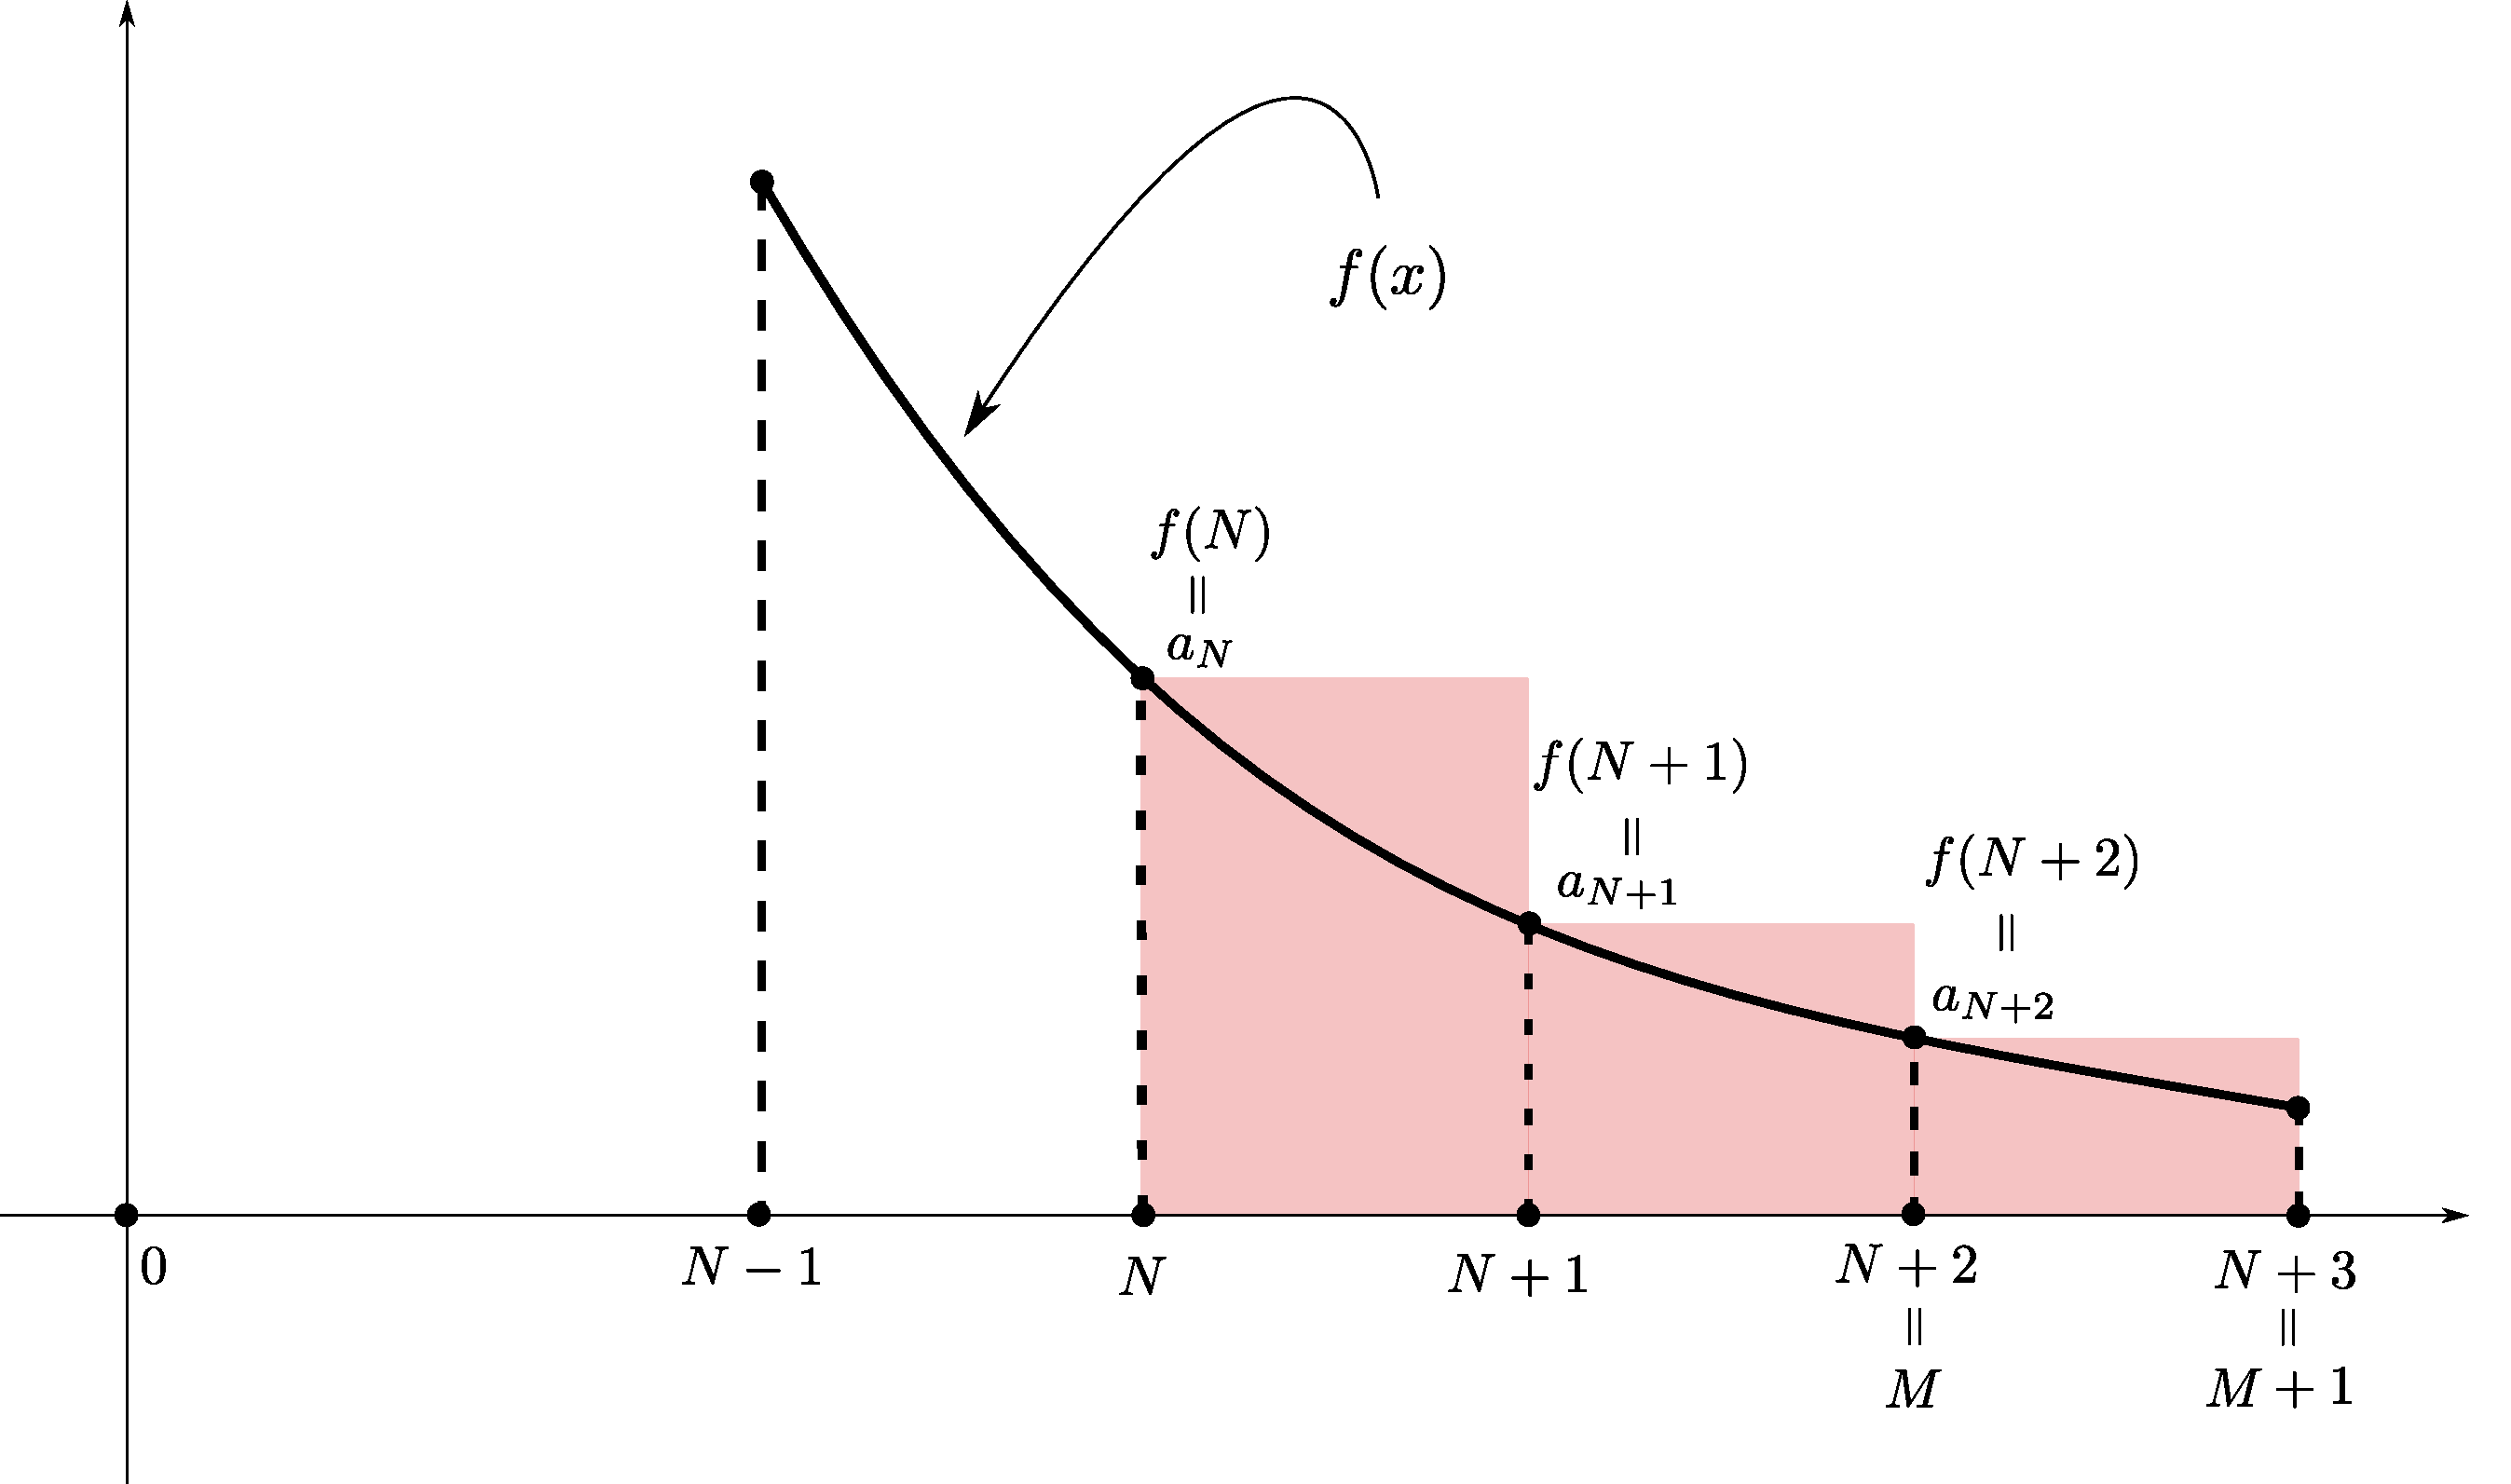
\includegraphics[width=0.63\linewidth]{Figuras/teste-integral-redimensionado1}
\caption{A área hachurada corresponde a soma $\sum_{n=N}^{M}a_n$. Observe que 
o valor desta soma é maior que a integral $\int_{N}^{M+1}f(x)\, dx$.}
\label{fig:teste-integral-redimensionado1}
\end{figure}

Para obter a segunda desigualdade raciocinamos de maneira análoga (bastando apenas
deslocar os retângulo que aparecem na figura acima para esquerda) como mostra
a Figura \ref{fig:teste-integral-redimensionado2}
\begin{figure}[h]
\centering
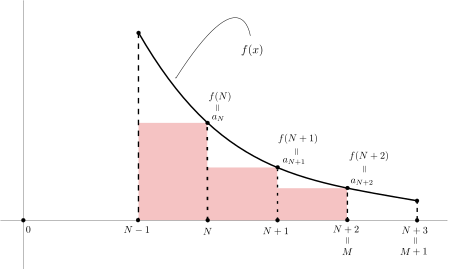
\includegraphics[width=0.63\linewidth]{Figuras/teste-integral-redimensionado2}
\caption{A área hachurada corresponde novamente a soma $\sum_{n=N}^{M}a_n$. Ela é
obtida simplesmente deslocando os retângulos da figura anterior para a esquerda. 
Observe que agora o valor desta soma é menor que a integral $\int_{N-1}^{M}f(x)\, dx$.}
\label{fig:teste-integral-redimensionado2}
\end{figure}
  
  

\end{proof}




\begin{corolario}\label{cor-crit-conv-p-series}
Fixado $p\in [0,+\infty)$, então temos que a $p$-série 
\[
\sum_{n=1}^{\infty} \frac{1}{n^p}
\] 
converge se $p>1$ e diverge se $0\leqslant p\leqslant 1$.
\end{corolario}

\begin{proof}
A prova deste corolário seguirá de uma aplicação do Teste da Integral
(Teorema \ref{teo-teste-da-integral}). Para isto vamos ter que apresentar 
a função $f$, a sequência $(a_n)_{n\in\mathbb{N}\cup\{0\}}$ e 
mostrar que todas as hipóteses do Teorema \ref{teo-teste-da-integral}
são satisfeitas. 

\medskip 
Para isto, podemos tomar $N=2$,
consideramos a sequência $(a_n)_{n\in\mathbb{N}\cup\{0\}}$ dada por $a_0=1$ e 
$a_n=n^{-p}$, para todo $n\in\mathbb{N}$. A função $f:[1,+\infty)\to\mathbb{R}$ 
é escolhida como sendo a função definida por
\[
f(x) = \frac{1}{x^p}.
\]

É imediato verificar que $f$ é monótona não-crescente (note que
$f'(x)<0,\ \forall x\in(1,\infty)$) e que $f(n) = n^{-p}$, para todo $n\in\mathbb{N}$.
Além do mais para todo $M>1$ temos que $f$ é integrável em $[1,M]$ e 
esta integral pode ser explicitamente calculada usando do Teorema Fundamental do Cálculo
como segue. 

Para $p$ positivo e  $p\neq 1$ temos:
\begin{align}\label{eq-aux1-p-series}
\int_{1}^{M}f(x)\, dx
&=
\int_{1}^{M}\frac{1}{x^p}\, dx
=
\int_{1}^{M}x^{-p}\, dx
=
\frac{1}{-p+1} x^{-p+1}\Big|_{1}^{M}
=
\frac{1}{1-p} x^{1-p}\Big|_{1}^{M}
\nonumber
\\[0.3cm]
&=
\frac{M^{1-p}-1}{1-p}
\end{align}

Para $p=1$ temos 
\begin{align}\label{eq-aux2-p-series}
\int_{1}^{M}f(x)\, dx
=
\int_{1}^{M}\frac{1}{x}\, dx
=
\ln(M)-\ln(1)= \ln(M).
\end{align}


Das igualdades \eqref{eq-aux1-p-series} e \eqref{eq-aux2-p-series}
temos que
\begin{align*}
\int_{1}^{\infty} \frac{1}{x^p}\, dx
=
\lim_{M\to\infty} \int_{1}^{M} \frac{1}{x^p}\, dx
&=
\begin{cases}
\displaystyle
\lim_{M\to\infty} \frac{M^{1-p}-1}{1-p},&\ \text{se}\ 0\leqslant p<1;
\\[0.5cm]
\displaystyle
\lim_{M\to\infty} \ln(M),&\ \text{se}\  p=1;
\\[0.5cm]
\displaystyle
\lim_{M\to\infty} \frac{M^{1-p}-1}{1-p},&\ \text{se}\ 1< p<+\infty;
\end{cases}
\\[0.5cm]
&=
\begin{cases}
\displaystyle
+\infty,&\ \text{se}\ 0\leqslant p<1;
\\[0.2cm]
\displaystyle
+\infty,&\ \text{se}\ 0\leqslant p=1;
\\[0.2cm]
\displaystyle
\frac{1}{p-1},&\ \text{se}\ 1< p<+\infty.
\end{cases}
\end{align*}

Finalmente, a prova segue das três igualdades acima e do Teste da Integral.
\end{proof}


\bigskip 
A seguir, lembramos outro importante critério, cuja a contra-positiva se constitui 
em um excelente dispositivo para avaliar se uma série diverge.


\begin{proposicao}\label{prop-conv-term-geral-vai-zero}
Seja $\sum_{n=0}^{\infty} a_n$ uma série de números complexos. 
Se $\sum_{n=0}^{\infty}a_n$ converge, então $a_n\to 0$, quando $n\to\infty$.
\end{proposicao}

\begin{proof}
Já que $\sum_{n=0}^{\infty} a_n$ converge, então sua sequência de somas parciais
forma uma sequência de Cauchy e portanto 
\[
\lim_{n\to\infty} |a_n| = \lim_{n\to\infty} |s_{n+1}-s_n| = 0.
\]
\end{proof}

Uma consequência deste resultado é que se $\sum_{n=0}^{\infty}a_n$
converge, então $(a_n)_{n\in\mathbb{N}\cup\{0\}}$ é uma sequência limitada.

Como veremos na próxima proposição uma 
forma conveniente de estudar a convergência de uma série de números complexos é 
via a série associada dos valores absolutos. Como no caso de séries de números 
reais, esta técnica não se aplica a todos os casos, mas ela é particularmente 
bastante poderosa, pois permite aplicarmos os testes de comparações para 
séries de números não-negativos.


\begin{definicao}
\label{def-conv-absoluta}
\index{Séries!absolutamente convergentes}
Dizemos que $\sum_{n=0}^{\infty} z_n$ converge absolutamente se a série 
$\sum_{n=0}^{\infty}|z_n|$ converge. 
\end{definicao}

\begin{proposicao}\label{prop-conv-abs-implica-conv}
Se a série $\sum_{n=0}^{\infty} z_n$ converge absolutamente, então 
ela é convergente.
\end{proposicao}


\begin{proof}
A ideia da prova consiste novamente em aplicar o critério de Cauchy.
Considere a sequência $(s_n)_{n\in\mathbb{N}\cup\{0\}}$ 
das somas parciais de $(z_n)_{n\in\mathbb{N}\cup\{0\}}$.
Como estamos assumindo que $\sum_{n=0}^{\infty} |z_n|$ converge, 
sabemos que dado $\varepsilon>0$ existe $n_0\in\mathbb{N}$ tal que 
se $m \geqslant n\geqslant n_0$ então 
\[
\Big| |z_n|+|z_{n+1}| +\ldots +|z_m|  \Big|<\varepsilon.
\]
Usando a Desigualdade Triangular e a desigualdade acima, temos
então para todo $m\geqslant n \geqslant n_0$
\begin{align*}
|s_{m}-s_n| = |z_{n}+z_{n+1}+\ldots+ z_{m}|
\leqslant  
\Big| |z_n|+|z_{n+1}| +\ldots +|z_m|  \Big|<\varepsilon.
\end{align*}
Como $\varepsilon>0$ é arbitrário, 
temos que $(s_n)_{n\in\mathbb{N}\cup\{0\}}$ é de Cauchy e portanto 
$\sum_{n=0}^{\infty} z_n$ converge.
\end{proof}


\bigskip 

Um dos exemplos mais importantes de séries que conhecemos é o das 
\textbf{séries geométricas}.
\index{Séries!geometricas}
Esta séries são definidas pelos termos de uma progressão geométrica e desempenham
papel fundamental, por exemplo, no estudo de séries de potências, como veremos adiante.
Esta séries são definidas a partir de uma sequência dada por $a_n = r^n$, 
para todo $n\in\mathbb{N}\cup\{0\}$, onde $r$ é um número real positivo.
Neste caso a sequência das somas parciais de $(a_n)_{n\in\mathbb{N}\cup\{0\}}$
é dada por 
\[
s_n = 1+r+r^2+\ldots r^{n-1}+r^n.
\]
Se $r\neq 1$ sabemos que 
\[
s_n = 1+r+r^2+\ldots r^{n-1}+r^n = \frac{1-r^{n+1}}{1-r}.
\]
Já que temos uma expressão explícita para $s_n$ 
é simples analisar a convergência ou divergência de tais séries. Bastando 
analisar se o limite, quando $n\to\infty$, do lado direito da igualdade acima
existe. E neste caso, se $0<r<1$ temos que $r^{n+1}\to 0$, quando $n\to\infty$,
e consequentemente
\[
\lim_{n\to\infty} s_n
=
\lim_{n\to\infty} \frac{1-r^{n+1}}{1-r}
= 
\frac{\displaystyle\lim_{n\to\infty} (1-r^{n+1})}{1-r} 
=
\frac{1}{1-r}.
\]

Por outro lado, se $r>1$ então temos que $r^{n+1}\to +\infty$, quando $n\to\infty$. 
Portanto
\[
\lim_{n\to\infty} s_n
=
\lim_{n\to\infty} \frac{1-r^{n+1}}{1-r}
= 
\frac{\displaystyle\lim_{n\to\infty} (1-r^{n+1})}{1-r} 
=
+\infty.
\]
No caso em que $r=1$, temos que 
\[
s_n = 1+1^1+1^2+\ldots+1^{n-1}+1^{n}=n+1 \xrightarrow{\ n\to\infty\ } +\infty.
\]


Em resumo, uma série geométrica $\sum_{n=0}^{\infty}r^n$, 
de termos positivos converge se, e somente se,
sua razão $r$ é estritamente menor do que um. 


\bigskip

Já que séries são definidas em termos de sequências de somas parciais. Algumas 
propriedades de sequências são herdadas pelas séries. Abaixo relacionamos alguns
deste fatos simples, mas que serão muito úteis a frente.

\begin{proposicao}
Sejam $\sum_{n=0}^{\infty}z_n$ e $\sum_{n=0}^{\infty}w_n$ duas séries convergentes.
Suponha que $\sum_{n=0}^{\infty}z_n = \alpha$ e $\sum_{n=0}^{\infty} w_n =\beta$.
Então  
\begin{itemize}
	\item a série $\sum_{n=0}^{\infty} cz_n$ converge para $c\alpha$,
	qualquer que seja $c\in\mathbb{C}$;
	
	\item a série $\sum_{n=0}^{\infty}(z_n +w_n)$ converge para $\alpha+\beta$.
\end{itemize}
\end{proposicao}

\begin{proof}
Para cada $n\in\mathbb{N}$, seja $s_n = z_0+z_1+\ldots z_n$, a $n$-ésima soma 
parcial da série $\sum_{n=0}^{\infty} z_n$. Note que, segue 
diretamente das propriedades
algébricas básicas de números complexos que 
a $n$-ésima soma parcial da série $\sum_{n=0}^{\infty} cz_n$ satisfaz a seguinte
igualdade $cz_1+cz_2+\ldots cz_n = cs_n$. Portanto 
\[
\sum_{n=0}^{\infty} cz_n
=
\lim_{n\to\infty} [cz_1+cz_2+\ldots+cz_n]
=
\lim_{n\to\infty} cs_n
=
c\lim_{n\to\infty} s_n
=
c\sum_{n=0}^{\infty} z_n
=
c\alpha.
\]
O que prova a validade do primeiro item da proposição. 

A prova do segundo é no mesmo espírito. Mantendo a notação do item anterior, 
seja $s_n$ a $n$-ésima soma parcial da série $\sum_{n=0}^{\infty}z_n$.
Defina $\widetilde{s}_n$ como sendo a $n$-ésima soma parcial da série
$\sum_{n=0}^{\infty}w_n$. Então, por definição, a $n$-ésima soma parcial da série
$\sum_{n=0}^{\infty}(z_n+w_n)$ satisfaz a seguinte igualdade
\[
(z_0+w_0)+(z_1+w_1)+\ldots+(z_n+w_n) = s_n+\widetilde{s}_n.
\]
Já que a soma de duas sequências convergentes é uma sequência convergente 
e o limite da soma é a soma dos limites, temos que 
a $n$-ésima soma parcial de $\sum_{n=0}^{\infty}(z_n+w_n)$ converge,
quando $n\to\infty$, e além do mais 
\begin{align*}
\sum_{n=0}^{\infty}(z_n+w_n)
&=
\lim_{n\to\infty}
\Big[ (z_0+w_0)+(z_1+w_1)+\ldots+(z_n+w_n) \Big]
\\
&= 
\lim_{n\to\infty}
(s_n+\widetilde{s}_n)
\\
&=
\lim_{n\to\infty}
s_n
+
\lim_{n\to\infty}
\widetilde{s}_n
=
\sum_{n=0}^{\infty}z_n + \sum_{n=0}^{\infty} w_n 
=
\alpha+\beta.
\end{align*}
O que finaliza a prova da proposição.
\end{proof}


\section{Sequências de Funções e Convergência}

Nesta seção vamos definir a noção de sequência de funções, um conceito que
generaliza o conceito de sequências numéricas. Em seguida, vamos discutir
alguns dos conceitos de convergência de sequências de funções. O objetivo
dos conceitos e dos resultados apresentados nesta seção é fornecer um 
arcabouço teórico para estudarmos séries de potencias no plano complexo. 

Diferentemente de sequências de números complexos ou reais, onde
temos um único conceito de convergência, quando
estamos tratando de sequência de funções, há diversas maneiras 
(com características bastante distintas, nem sempre sendo possível 
hierarquizá-las no sentido de apontar qual é a ``melhor'' delas) de 
se definir convergência. Nesta seção vamos apresentar discutir 
sobre três noções de convergência para sequência de funções:
\begin{itemize}
	\item convergência pontual; 
	\item convergência uniforme;
	\item convergência uniforme nas partes compactas.
\end{itemize}

A noção de convergência pontual, como veremos a seguir, é mais simples de 
ser apresentada e de se trabalhar. Por outro lado, a função limite 
obtida por convergência pontual pode não herdar propriedades que
os elementos da sequência de funções possui. Por exemplo, o limite pontual
de uma sequência de funções contínuas pode não ser uma função contínua
(Exemplo \ref{ex-lim-Somas-desc}). 
Ou seja,
é possível construir uma sequência de funções, onde cada elemento desta sequência é 
uma função contínua. Porém a função obtida como limite pontual desta sequência, 
não herda a propriedade de continuidade. Isto alerta para o fato de
que, apesar de ser muito importante e poderosa, a convergência pontual 
pode não ser capaz de fornecer várias informações que eventualmente estaríamos
interessados. 

Para evitar algumas dificuldades técnicas, oriundas do conceito de convergência pontual,
vamos introduzir um outro conceito de convergência de sequência de funções. O conceito de 
convergência uniforme. Embora, seja mais difícil trabalhar com 
este conceito, temos a vantagem de que 
quando conseguimos provar que uma determinada 
sequência de funções converge uniformemente para alguma função complexa, 
então seremos capazes de extrair muito 
mais informações sobre esta função limite! 
Como já deve estar suspeitando o leitor, em geral, não será simples
nem viável provar que uma determinada sequência de funções converge uniformemente 
para uma função limite. Mas em muito casos interessantes será possível mostrar
que se restringimos a nossa sequência de funções, à subconjuntos compactos do
seu domínio, a tarefa de mostrar a convergência uniforme 
poderá ser realizada. A grande vantagem desta abordagem é que mesmo sendo 
este conceito de convergência um pouco mais fraco do que o conceito de convergência
uniforme seremos capazes de mostrar que a função limite preserva diversas propriedades
das ``funções aproximantes''. 
 

O principal exemplo de sequência de funções que o leitor deve ter em mente,
quando estiver lendo esta seção, é o da sequência dos polinômios de 
Taylor de uma série de potências. Vamos estudar
em detalhes esta importante classe de exemplos na Seção \ref{ex-lim-Somas-desc}.


\bigskip 

Em toda esta seção $U\subset\mathbb{C}$ denotará sempre um  
conjunto aberto, que pode ser limitado ou ilimitado. Não há necessidade 
também de assumir que $U$ seja conexo. Isto é, os resultados a serem 
apresentados nesta seção valem para o caso em que $U$ é desconexo. 

\begin{definicao}[Sequência de Funções Complexas]
Dizemos que $(f_n)_{n\in\mathbb{N}\cup\{0\}}$ 
é uma sequência de funções complexas, definidas em $U$, se
\index{Sequência!de funções complexas}
para cada $n\in\mathbb{N}\cup\{0\}$ o termo $f_n$ denota uma 
função definida em $U$ e tomando valores complexos, isto é,  
$f_n:U\to\mathbb{C}$ é uma função.
\end{definicao}

Uma observação importante sobre a definição acima é que em uma sequência
de funções $(f_n)_{n\in\mathbb{N}\cup\{0\}}$ todas as funções da sequência 
estão definidas no mesmo domínio, que aqui convencionamos como sendo um conjunto 
$U\subset \mathbb{C}$ aberto. 

\begin{exemplo}\label{exemplo-seq-func-disco}
Seja $U=\mathbb{D}\subset\mathbb{C}$ o disco unitário. Para cada $n\in\mathbb{N}\cup\{0\}$
seja $f_n:\mathbb{D}\to\mathbb{C}$ a função dada por
\[
f_n(z) = z^n, \qquad \forall\, z\in\mathbb{D}.
\]
Então $(f_n)_{n\in\mathbb{N}\cup\{0\}}$ define uma sequência de funções complexas 
em $\mathbb{D}$.
\end{exemplo}

Sempre que estivermos tratando de sequência de funções é importante deixar claro 
qual é domínio onde as funções da nossa sequência estão definidas. A rigor, a
sequência definida no próximo exemplo é completamente distinta (apesar de sua aparência)
daquela do exemplo anterior

\begin{exemplo}\label{exemplo-seq-func-plano}
Seja $U=\mathbb{C}$. Para cada $n\in\mathbb{N}\cup\{0\}$
seja $g_n:\mathbb{C}\to\mathbb{C}$ a função dada por
\[
g_n(z) = z^n, \qquad \forall\, z\in\mathbb{C }.
\]
Então $(g_n)_{n\in\mathbb{N}\cup\{0\}}$ define uma sequência de funções complexas 
em $\mathbb{C}$.
\end{exemplo}

Apesar da semelhança das leis de $f_n$ e $g_n$, 
apresentadas nos dois exemplos anteriores, 
estas funções devem ser reconhecidas como funções distintas, 
pois possuem domínios distintos. 
Obviamente, $f_n$ pode ser vista 
como a restrição de $g_n$ ao disco unitário. Mas o leitor deve estar atento
que a rigor $f_n$ e $g_n$ devem ser tratadas como funções distintas.
A importância de se fazer tal distinção ficará ainda mais clara, quando introduzirmos 
os conceitos de convergência. Por exemplo, veremos, a frente, que a sequência 
$(f_n)_{n\in\mathbb{N}\cup\{0\}}$ será convergente (no sentido da convergência pontual - a ser definida), porém a sequência $(g_n)_{n\in\mathbb{N}\cup\{0\}}$ não será pontualmente convergente!


\begin{exemplo}
Sejam $U=\mathbb{D}\subset\mathbb{C}$ o disco unitário e 
$(f_n)_{n\in\mathbb{N}\cup\{0\}}$ a sequência de funções 
definidas no Exemplo \ref{exemplo-seq-func-disco}.
Para cada $n\in\mathbb{N}\cup\{0\}$
defina a função $S_n:\mathbb{D}\to\mathbb{C}$ como sendo
\[
S_n(z) = 1+z+z^2+\ldots+z^n = \sum_{j=0}^{n} f_n(z), \qquad \forall\, z\in\mathbb{D}.
\]
Então $(S_n)_{n\in\mathbb{N}\cup\{0\}}$ define uma sequência de funções complexas 
em $\mathbb{D}$. O leitor pode observar que esta sequência de funções é o análogo, 
para sequência de funções, do conceito de sequência de somas parciais. 
Além do mais, para cada $z\in\mathbb{D}$ fixado a sequência numérica
$(S_n(z))_{n\in\mathbb{N}\cup\{0\}}$ representa 
as somas parciais de uma série geométrica de razão $z$. 
\end{exemplo}



\begin{definicao}[Sequência de Somas Parciais de uma sequência de funções]
\label{def-seq-somasparciais-funcoes}
Seja $(f_n)_{n\in\mathbb{N}\cup\{0\}}$ uma sequência de funções complexas 
definida em $U$. Definimos a sequência das somas parciais
de $(f_n)_{n\in\mathbb{N}\cup\{0\}}$, como sendo uma nova sequência de funções 
complexas $(S_n)_{n\in\mathbb{N}\cup\{0\}}$ definidas em $U$, onde 
para cada $n\in\mathbb{N}\cup\{0\}$, a função $S_n:U\to\mathbb{C}$ é dada por 
\[
S_n(z) = f_0(z)+f_1(z)+f_2(z)+\ldots+f_n(z) = \sum_{j=0}^n f_j(z),
\qquad \forall z\in U.
\]
\end{definicao}


Os exemplos que devem aparecer com mais frequência neste texto relacionados
a sequências de funções e suas respectivas sequências de somas parciais são
os seguintes: 

\begin{exemplo}\label{exe-seq-fun-series-pot}
Dada uma sequência numérica $(a_n)_{n\in\mathbb{N}\cup\{0\}}$ arbitrária 
de números complexos e um aberto $U\subset\mathbb{C}$, 
defina a seguinte sequência de funções complexas 
$(f_n)_{n\in\mathbb{N}\cup\{0\}}$, onde para cada $n\in\mathbb{N}$, 
a função $f_n:U\to\mathbb{C}$ é dada por
\[
f_n(z) = a_nz^n, \qquad \forall z\in U.
\] 

Então a sequência das somas parciais de $(f_n)_{n\in\mathbb{N}\cup\{0\}}$,
denotada por $(S_n)_{n\in\mathbb{N}\cup\{0\}}$ é dada por 
\[
S_n(z) = a_0+a_1z+a_2z^2+\ldots +a_{n-1}z^{n-1}+a_nz^n = \sum_{j=0}^n a_jz^j, 
\qquad \forall z\in U.
\]
\end{exemplo}



\begin{exemplo}\label{ex-somas-parciais-zeta}
Seja $U=\{z\in\mathbb{C}: \Re(z)>1\}$ e $\log:\mathbb{C}\setminus L_{\pi}\to\mathbb{C}$
o ramo principal do logaritmo.
Seja $(f_n)_{n\in\mathbb{N}}$ a sequência de funções complexas, onde para cada 
$n\in\mathbb{N}$, a função $f_n:U\to\mathbb{C}$ é definida por
\[
f_n(z) = \exp(-z\log n) = \frac{1}{\exp(z\log n)} = \frac{1}{n^z}.
\]
Então $(S_n)_{n\in\mathbb{N}}$, a sequência das somas parciais de $(f_n)_{n\in\mathbb{N}}$ é 
dada por
\[
S_n(z) = 1+\frac{1}{2^z}+\ldots+\frac{1}{n^z} = \sum_{j=1}^n \frac{1}{j^z}.
\]
\end{exemplo}



\begin{definicao}[Convergência Pontual]
\index{Convergência!pontual}
Sejam $U\subset\mathbb{C}$ um conjunto aberto e $(f_n)_{n\in\mathbb{N}\cup\{0\}}$
uma sequência de funções complexas definidas em $U$. Dizemos que a sequência de
funções $(f_n)_{n\in\mathbb{N}\cup\{0\}}$ \textbf{converge pontualmente} para uma função complexa $f:U\to\mathbb{C}$ se para cada $z\in U$ temos 
\[
\lim_{n\to\infty} f_n(z) = f(z).
\]
\end{definicao}


Do ponto de vista da definição forma de limite a noção de convergência pontual
pode ser reformulada da seguinte forma. 
Seja $(f_n)_{n\in\mathbb{N}\cup\{0\}}$ uma sequência de funções complexas
definidas em $U$ que converge pontualmente para $f:U\to\mathbb{C}$. Então podemos
afirmar que dado $\varepsilon>0$ e fixado $z\in U$, 
existe $n_0\equiv n_0(z,\varepsilon)\in\mathbb{N}$
tal que se $n\geqslant n_0$ então 
\[
|f_n(z)-f(z)|<\varepsilon.
\]
Isto quer dizer que, fixado $\varepsilon>0$ então 
a imagem de $z$ por $f$ está $\varepsilon$-próxima da 
imagem de $z$ por $f_n$, sempre que $n$ for maior ou igual a 
$n_0(\varepsilon,z)$ que pode depender de $\varepsilon$ e eventualmente 
também de $z$.
Observe que não há nenhum conflito, com a observação acima, em dizer que existe 
$w\in U$ tal que 
\[
|f_{n_0(\varepsilon,z)}(w)-f(w)| \geqslant \varepsilon 
\]

\begin{figure}[h]
\centering
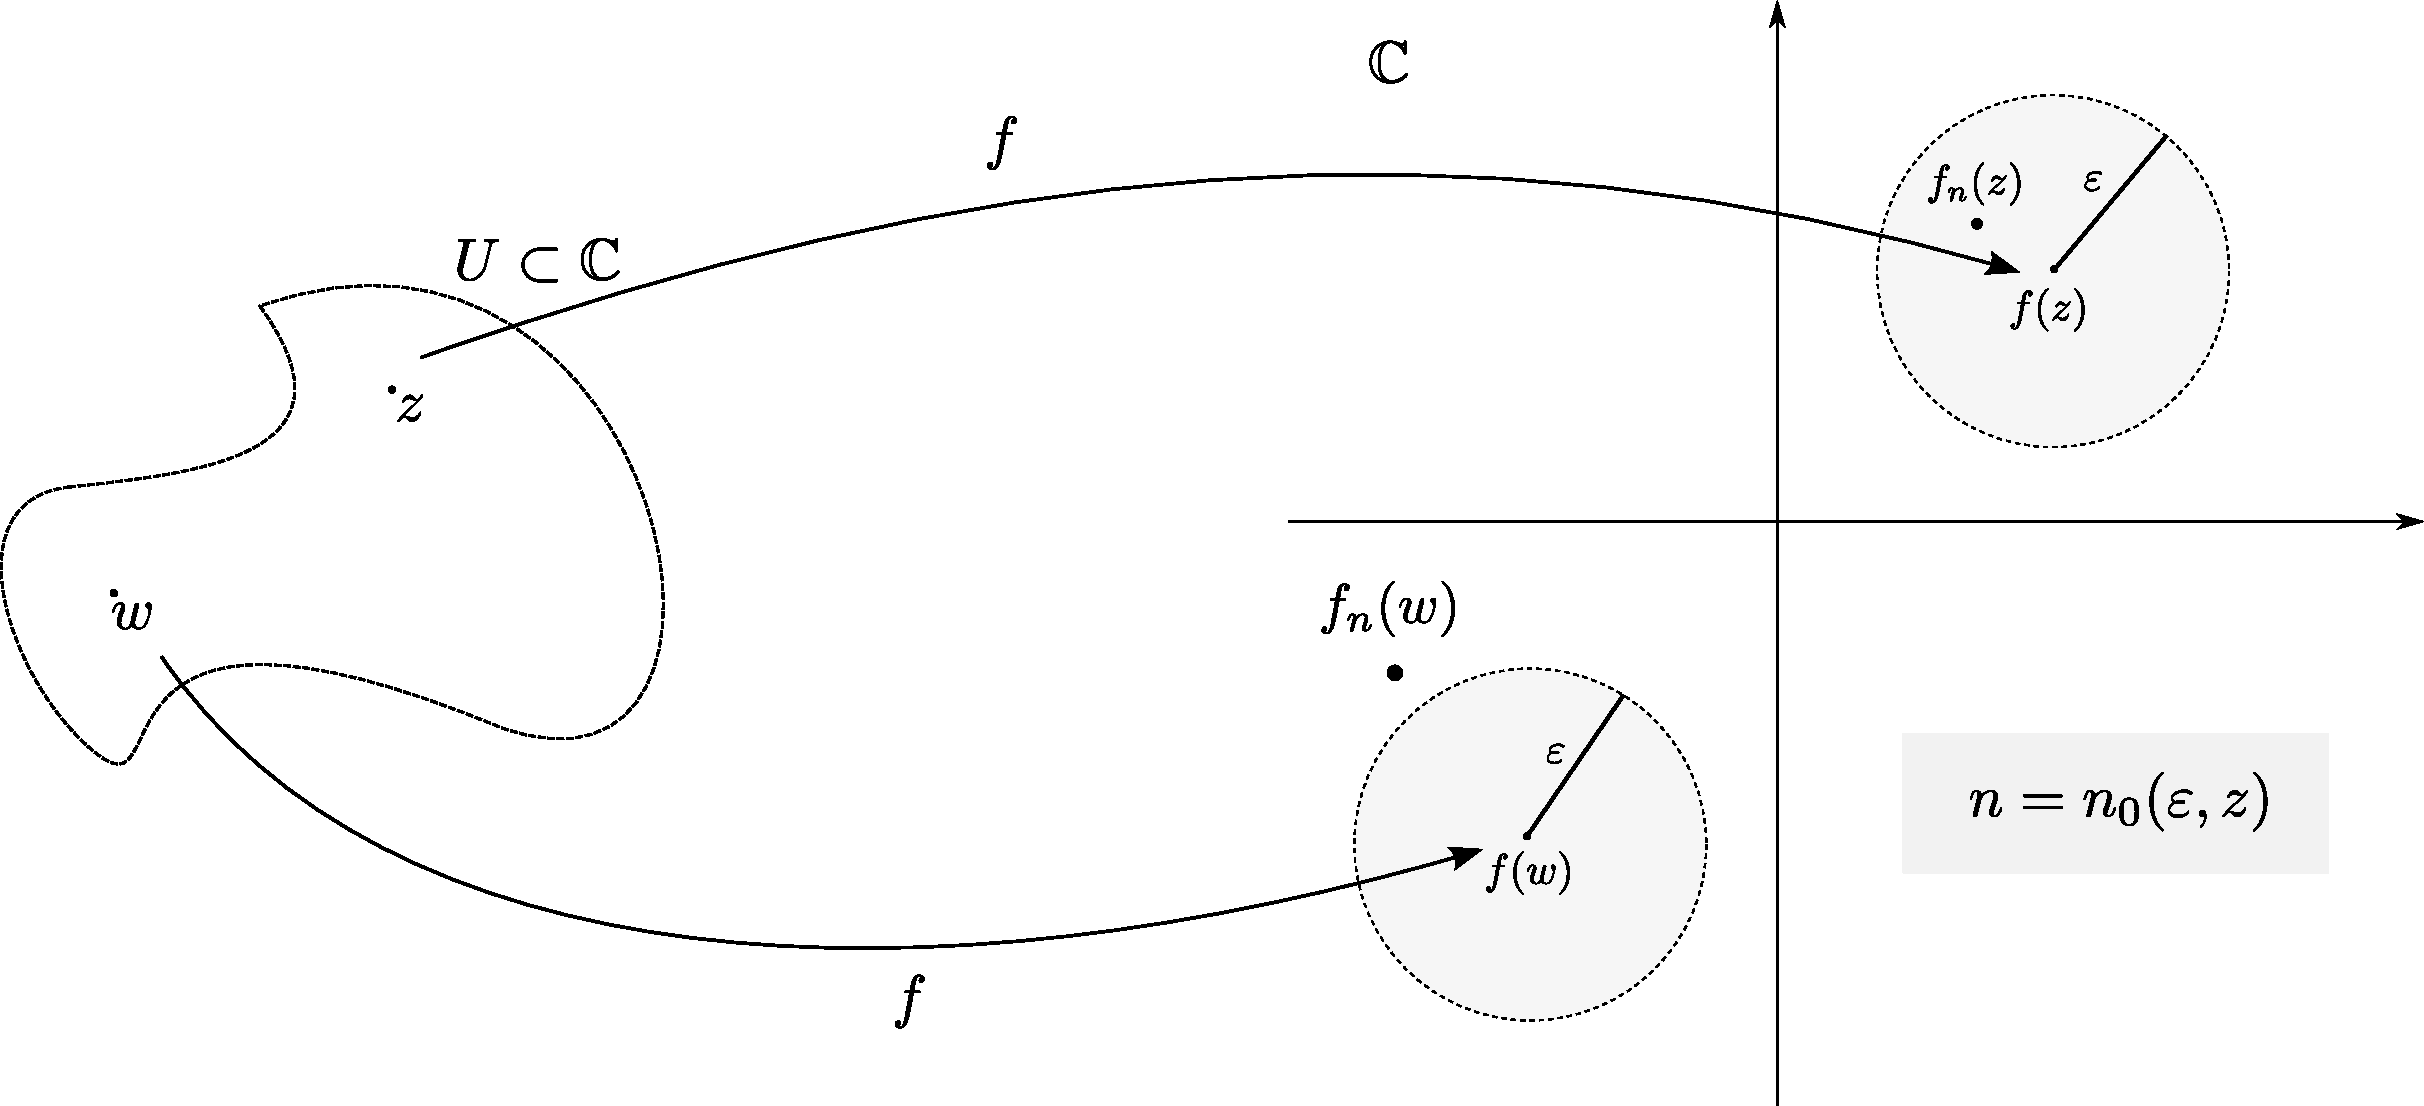
\includegraphics[width=0.95\linewidth]{Figuras/convergencia-pontual-redimensionado}
\caption{Na figura acima, temos uma sequência de funções 
$(f_n)_{n\in\mathbb{N}\cup\{0\}}$ converge pontualmente para $f$. 
Mas note que pode acontecer da convergência ser mais ``lenta'' para alguns pontos. Nesta
figura vimos que $f_n(z)$ está $\varepsilon$ próximo de $f(z)$ mas o mesmo não ocorre
para $f_n(w)$. Como sabemos que $f_n(w)$ converge para $f(w)$ o que está acontecendo
nesta situação é que é necessário tomar o índice $n$ em $f_n(w)$ muito maior do 
que $n_0(\varepsilon,z)$.}
\label{fig:convergencia-pontual-redimensionado}
\end{figure}


A desigualdade acima poderia ser válida inclusive para uma quantidade finita 
de índices consecutivos a $n_0(\varepsilon,z)$, isto é, para 
$n_0(\varepsilon,z)+k$, com $k\in\{1,\ldots,m\}$, ou seja, poderíamos ter ainda
\[
|f_{n_0(\varepsilon,z)+k}(w)-f(w)| \geqslant \varepsilon,
\qquad k\in\{1,\ldots,m\}. 
\] 
Mas é claro, como a propriedade que define a convergência pontual exige que
\[
\lim_{n\to\infty} f_n(w) = f(w),
\]
e por isto, sabemos que deverá existir algum natural $n_1(\varepsilon,w)>n_0(\varepsilon,z)$ (que poderia talvez ser muito maior que $n_0(\varepsilon,z)$) 
satisfazendo
\[
|f_{n}(w)-f(w)| < \varepsilon, \qquad \forall n\geqslant n_1(\varepsilon,w).
\]

Se $(f_n)_{n\in\mathbb{N}\cup\{0\}}$ é uma sequência de funções complexas definidas em
$U$ que converge pontualmente para $f:U\to\mathbb{C}$, então é comum às vezes 
nos referirmos a $f_n$ como uma aproximante de $f$.


\bigskip 
Vamos analisar se as sequências $(f_n)_{n\in\mathbb{N}\cup\{0\}}$ 
e $(g_n)_{n\in\mathbb{N}\cup\{0\}}$ dos Exemplos \ref{exemplo-seq-func-disco}
e \ref{exemplo-seq-func-plano} e verificar se elas convergem pontualmente para alguma função.


Vamos considerar primeiro a sequência de funções do Exemplo \ref{exemplo-seq-func-disco}.
Neste caso, $U=\mathbb{D}$ e para cada $n\in\mathbb{N}$ temos que 
$f_n:\mathbb{D}\to\mathbb{C}$ é dada por $f_n(z)=z^n$. Como qualquer ponto $z\in\mathbb{D}$
pode ser representado em coordenadas polares na forma $z=re^{i\theta}$, onde $0\leqslant r< 1$
e $\theta\in [0,2\pi)$ temos que 
\[
\lim_{n\to\infty} f_n(z) 
= 
\lim_{n\to\infty} z^n 
=
\lim_{n\to\infty} (re^{i\theta})^n
=
\lim_{n\to\infty}r^n e^{in\theta}=0.
\]
Como $z\in\mathbb{D}$ é arbitrário então temos que $(f_n)_{n\in\mathbb{N}\cup\{0\}}$ 
converge pontualmente para a função identicamente nula em $U$, isto é, 
$f:U\to\mathbb{C}$ dada por $f(z)=0$ para todo $z\in\mathbb{D}$.

Por outro lado, podemos ver que a sequência apresentada no Exemplo 
\ref{exemplo-seq-func-plano} não converge pontualmente para nenhuma função 
complexa. De fato, basta observar que existe um ponto 
(na verdade, poderíamos tomar qualquer ponto no conjunto $\mathbb{C}\setminus (\mathbb{D}\setminus\{1\})$) $z\in \mathbb{C}$ para o qual $g_n(z)$ não converge. Por exemplo, tome 
$z=1+i$. Representando este ponto em coordenadas polares, $z=\sqrt{2}e^{i\pi/4}$,
podemos calcular facilmente $z^n = 2^{n/2}e^{in\pi/4}$. 
Já que $|z^n|=2^{n/2}\xrightarrow{\ n\to\infty\ }+\infty$,
segue que $g_n(z)=z^n$ não converge. Portanto não existe nenhuma função $f:\mathbb{C}\to\mathbb{C}$
tal que $(g_n)_{n\in\mathbb{N}\cup\{0\}}$ converge pontualmente para $g$.


\medskip 

Vamos analisar agora a convergência das somas 
parciais do Exemplo \ref{ex-somas-parciais-zeta}.
Neste exemplo, a sequência que gera as somas parciais é definida no 
conjunto $\{z\in\mathbb{C}: \Re(z)>1\}$ e dada por $f_n(z)= \exp(-z\ln n) = 1/n^z$
e as somas parciais são dadas por 
\[
S_k(z) = \sum_{n=1}^{k}\frac{1}{n^z}.
\]
Vamos mostrar, para cada $z\in\{z\in\mathbb{C}: \Re(z)>1\}$ 
que  $(S_n)_{n\in\mathbb{N}}$ converge para um função complexa
$\zeta:\{z\in\mathbb{C}: \Re(z)>1\}\to\mathbb{C}$. 

De fato, para cada $n\in\mathbb{N}$ e $z\in\{z\in\mathbb{C}: \Re(z)>1\}$ 
temos
\[
|f_n(z)| = \frac{1}{n^z}  = |\exp(-z\ln n)| = \exp(-\Re(z)\ln n) = \frac{1}{n^{\Re(z)}}.
\]
Pela desigualdade triangular temos a seguinte estimativa 
\[
|S_k(z)| 
\leq 
\sum_{n=1}^{k}\left|\frac{1}{n^z}\right|
=
\sum_{n=1}^{k} \frac{1}{n^{\Re(z)}}.
\]
Note que no lado direito da igualdade acima, temos a $k$-ésima soma parcial
de uma $p$-série, onde $p=\Re(z)$. 
Já que $z\in\{z\in\mathbb{C}: \Re(z)>1\}$ segue do Corolário \ref{cor-crit-conv-p-series} 
que 
\[
\sum_{n=1}^{\infty}\left|\frac{1}{n^z}\right|
=
\sum_{n=1}^{\infty} \frac{1}{n^{\Re(z)}}.
\]
converge. Então segue da Proposição \ref{prop-conv-abs-implica-conv} que a série
abaixo é convergente
\[
\sum_{n=1}^{\infty} f_n(z) \equiv \sum_{n=1}^{\infty} \frac{1}{n^z}
\]
para cada $z\in\{z\in\mathbb{C}: \Re(z)>1\}$. Logo
existe um número complexo que chamaremos de 
$\zeta(z)$ tal que 
\[
\zeta(z) = \sum_{n=1}^{\infty} \frac{1}{n^z}.
\]

A análise acima mostra que podemos associar a cada $z\in\{z\in\mathbb{C}: \Re(z)>1\}$ 
um número complexo $\zeta(z)\in\mathbb{C}$ dado pelo série acima.
Desta forma temos uma função complexa $\zeta:\{z\in\mathbb{C}: \Re(z)>1\}\to\mathbb{C}$
que é o limite pontual da sequência $(S_n)_{n\in\mathbb{N}}$. 
Esta função é chamada de \textbf{função zeta de Riemann}.
\index{Função!zeta de Riemann}
Na verdade, há um pequeno abuso de terminologia, pois a função que de fato é chamada
de função zeta de Riemann é uma função complexa definida no conjunto $\mathbb{C}\setminus\{1\}$
e a função que temos acima, é na verdade a restrição da verdadeira função zeta de Riemann
ao semi-plano $\{z\in\mathbb{C}: \Re(z)>1\}$.
Para não ter perigo de confusão, nesta seção o que vamos chamar 
de função zeta de Riemann é a
função que acabamos de definir acima, e seu domínio é precisamente o 
semi-plano $\{z\in\mathbb{C}: \Re(z)>1\}$.

Como para cada $n\in\mathbb{N}$, temos que 
temos que a função $z\longmapsto S_n(z)$ é contínua e mais ainda holomorfa
na região $\{z\in\mathbb{C}: \Re(z)>1\}$; e obtida como limite pontual de $(S_n)_{n\in\mathbb{N}}$, duas perguntas que surgem naturalmente são:
\begin{itemize}
	\item a função $\zeta:\{z\in\mathbb{C}: \Re(z)>1\}\to\mathbb{C}$ é uma função contínua?  
	\item a função $\zeta:\{z\in\mathbb{C}: \Re(z)>1\}\to\mathbb{C}$ é uma função holomorfa?
\end{itemize}

Na verdade, a resposta para as duas perguntas é positiva. Mas como vamos
ver a seguir, responder estas perguntas vão requerer uma análise um pouco mais
refinada sobre a convergência da sequência $(S_n)_{n\in\mathbb{N}}$.


\begin{exemplo}\label{ex-lim-Somas-desc}
Considere a sequência de funções complexas $(f_n)_{n\in\mathbb{N}\cup\{0\}}$,
onde para cada $n\in\mathbb{N}\cup\{0\}$ a função 
$f_n:\mathbb{C}\to\mathbb{C}$ é dada por 
\begin{align*}
f_n(z) = \frac{|z|^2}{(1+|z|^2)^n}.
\end{align*}
Seja $(S_n)_{n\in\mathbb{N}\cup\{0\}}$ a sequência das somas parciais de $(f_n)_{n\in\mathbb{N}\cup\{0\}}$. 

\medskip 
Vamos mostrar a seguir que $(S_n)_{n\in\mathbb{N}\cup\{0\}}$ converge pontualmente para a função 
$S:\mathbb{C}\to\mathbb{C}$ dada por
\[
S(z) 
=
\begin{cases}
0,&\text{se}\ z=0;\\
1+|z|^2,&\text{se}\ z\neq 0.
\end{cases}
\]
Fornecendo Assim um exemplo de uma sequência 
$(S_n)_{n\in\mathbb{N}\cup\{0\}}$
de funções complexas \textbf{contínuas}
convergindo para uma função complexa descontínua 
(note que a função $S$ não é contínua na origem). 

Vamos então verificar que 
\[
\lim_{n\to\infty} S_n(z) = S(z), \qquad \forall z\in\mathbb{C}.
\]
Para isto vamos considerar separadamente os casos $z=0$ e $z\neq 0$.

No caso $z=0$, temos para todo $n\geqslant 0$ que
\[ 
S_n(0) = \sum_{j=0}^n f_j(0) = 0
\]
Logo $S_n(0)\xrightarrow{\ n\to\infty\ }0=S(0)$.

No caso $z\neq 0$, 
\[ 
S_n(z) 
= \sum_{j=0}^n f_j(z) 
= \sum_{j=0}^n \frac{|z|^2}{(1+|z|^2)^n}
= |z|^2 \sum_{j=0}^n \frac{1}{(1+|z|^2)^n}.
\]
Já  que para cada $z\neq 0$ fixado, temos $(1+|z|^2)>1$, é imediato verificar 
que $S_n(z)$ é a $n$-ésima soma parcial de uma série geométrica de razão 
\[
r = \frac{1}{1+|z|^2}<1.
\]

Portanto podemos obter explicitamente a expressão do limite de $S_n(z)$,
quando $n\to\infty$, como segue
\begin{align*}
\lim_{n\to\infty} S_n(z) 
&=
|z|^2 \lim_{n\to\infty}\sum_{j=0}^n \frac{1}{(1+|z|^2)^j}
=
|z|^2 
\sum_{n=0}^{\infty} r^n
=
|z|^2 \frac{1}{1-r}
\\
&
=
|z|^2 \ \frac{1}{1- \frac{1}{1+|z|^2} }
\\
&=
1+|z|^2.
\\
&=
S(z).
\end{align*}
\end{exemplo}



Em resumo, o exemplo acima mostra que o limite pontual de uma soma 
de funções contínuas pode \textbf{não} ser uma função contínua. Deixando bem claro
que mesmo a questão da continuidade da função zeta Riemann é um fato
não-trivial. Além do mais, questões similares a estas são relevantes e naturais
também no contexto de séries de potências. Na próxima seção 
vamos estudá-las detalhadamente.


\section{Séries de Potências}
\label{sec-series-potencias}

Nesta seção vamos apresentar a definição e estudar algumas propriedades
básicas sobre séries de potências no plano complexo. 

Vamos usar séries de potências para dar importantes exemplos
de funções analíticas. Ao longo da seção o leitor deve notar
que alguns dos resultados apresentados aqui 
se assemelham a outros resultados familiares que aparecem até 
mesmo nos cursos introdutórios de Cálculo. 




\subsection{Séries de Potências Centradas na Origem}
\label{subsec-series-pot-centro-zero}
\begin{definicao}[Séries de Potências]
\label{def-series-de-potencias}
\index{Séries!de potências}
Sejam $(a_n)_{n\in\mathbb{N}\cup\{0\}}$ uma sequência 
de número complexos e $z\in\mathbb{C}$ um número complexo fixado. 
Considere a sequência $(a_nz^n)_{n\in\mathbb{N}\cup\{0\}}$.
A série numérica associada a esta sequência, isto é,
\[
\sum_{n=0}^{\infty} a_n\, z^n,
\]
é chamada série de potências de centro em $0$.
\end{definicao}


Convidamos o leitor a reler, neste momento, 
cuidadosamente a definição de séries 
numéricas (Definição \ref{def-series-num-complexos}).

Ela diz que a série gerada pela sequência
$(a_nz^n)_{n\in\mathbb{N}\cup\{0\}}$ 
como objeto matemático é na verdade outra sequência 
a chamada sequência de somas parciais, que será denotada por $(S_n(z))_{n\in\mathbb{N}\cup\{0\}}$ e dada por

\begin{align*}
S_0(z) 	&= a_0
\\
S_1(z) 	&= a_0+a_1z
\\
S_2(z) 	&= a_0+a_1z+a_2z^2
\\
S_3(z)	&= a_0+a_1z+a_2z^2+a_3z^3
\\
		&\vdots	
\\
S_n(z)	&= a_0+a_1z+a_2z^2+\ldots+a_nz^n
\\
		&\vdots	
\end{align*}

Portanto seguindo a Definição \ref{def-series-num-complexos} dizemos que
a série de potências 
\[
\sum_{n=0}^{\infty} a_n\, z^n,
\]
converge, se a sequência das somas parciais $(S_n(z))_{n\in\mathbb{N}\cup\{0\}}$ 
converge, isto é, 
existe um número complexo, que sugestivamente será chamado de $f(z)$, tal que
\[
\lim_{n\to\infty} S_n(z) = f(z).
\]


Olhando apenas para os pontos $z\in\mathbb{C}$ 
onde $(S_n(z))_{n\in\mathbb{N}\cup\{0\}}$
converge, podemos definir uma função. A função que leva $z$ em 
$\lim_{n\to\infty}S_n(z)=f(z)$.
A função $f$ definida desta maneira tem seu domínio dado precisamente pelo conjunto 
\[
\mathrm{dom}(f) = 
\Big\{ z\in\mathbb{C} :  \ \text{existe} \ \lim_{n\to\infty}S_n(z)  \Big\}.
\]

Apesar de muito simples, esta descrição, do domínio de $f$, 
é de pouca utilidade. Por exemplo, se estivermos interessados
em estudar continuidade ou diferenciabilidade de $f$ 
em um ponto $z_0$ de seu domínio, vamos precisar
saber, além de outras coisas, se $f$ também está bem definida em todos os pontos de algum disco
com centro em $z_0$ e raio positivo. 
Em outras palavras, do ponto de vista mais clássico de
se fazer uma teoria de cálculo, nos interessa mais é saber quem é o interior 
do domínio de $f$, que seguindo a notação da seção sobre topologia no 
plano complexo era denotado por $\mathrm{int}(\mathrm{dom}(f))$.


\medskip 
Observamos que determinar exatamente o domínio da função $f$, dada acima,
pode ser uma tarefa extremamente complicada. 
Por outro lado, provaremos, a seguir, um resultado incrível 
(Teorema \ref{teo-exist-raio-conv})
que afirma que este domínio é ``moralmente'' 
um disco. 
Mais precisamente, vamos demonstrar que existe um único $R\in [0,+\infty]$ tal que
\[
\mathrm{dom}(f)\subset \overline{D(0,R)} 
\qquad \text{e} \qquad 
\mathrm{int}(\mathrm{dom}(f)) = D(0,R),
\]
e além do mais, este número $R$ depende apenas da sequência 
$(a _n)_{n\in\mathbb{N}\cup\{0\}}$ e dado explicitamente por
\[
R 
= 
\begin{cases}
\frac{1}{ \displaystyle\limsup_{n\to\infty} \sqrt[n]{|a_n|} },&
\ \ \text{se}\ \limsup_{n\to\infty} \sqrt[n]{|a_n|}\neq 0;
\\[1.0cm]
+\infty,&\ \ \text{se}\ \limsup_{n\to\infty} \sqrt[n]{|a_n|}=0,
\end{cases}
\]
onde 
\[
\limsup_{n\to\infty} \sqrt[n]{|a_n|}
\equiv 
\lim_{n\to\infty} \left[ \sup \Big\{ \sqrt[n]{|a_n|}, \sqrt[n+1]{|a_{n+1}|}, \sqrt[n+2]{|a_{n+2}|},\ldots  \Big\} \right].
\]

Se $R=0$ então a série de potências só converge na origem. 
Para $R=+\infty$ a série converge para qualquer escolha de $z\in \mathbb{C}$
o que motiva usar a notação $D(0,+\infty)\equiv \mathbb{C}$.


\bigskip 
Do que foi enunciado acima, 
concluímos que o domínio de $f$ é sempre o disco aberto de centro zero 
e raio $R$ unido eventualmente 
com mais alguns pontos do bordo deste disco (a circunferência $\partial D(0,R)$).
Como no caso de séries de potências de números reais, o número $R$ 
é chamado de raio de convergência da série de potencias e $D(0,R)$
o disco de convergência.  

Após feita as provas dos fatos mencionados acima teremos preparado o 
terreno para olhar para séries de potências como limites de sequências
de funções. Antes porém vamos gostaríamos de acrescentar alguns comentários
sobre o raio de convergência. 



\bigskip

À primeira vista a expressão de $R$ pode parecer assustadora, mas
observamos que em vários exemplos práticos, teremos
\[
\limsup_{n\to\infty} \sqrt[n]{|a_n|} = \lim_{n\to\infty} \sqrt[n]{|a_n|}.
\]
Ou seja, o ``limsup'' é simplesmente o limite. 
Na verdade, isto sempre acontece quando o limite existe.
Mas é importantíssimo observar que nem toda sequência da forma $\sqrt[n]{|a_n|}$
possui limite em $[0,+\infty]$. 
Por outro lado, $\limsup_{n\to\infty} \sqrt[n]{|a_n|}$
está sempre bem definido como um ponto em $[0,+\infty]$. 
Portanto é sempre lícito escrever 
\[
\limsup_{n\to\infty} \sqrt[n]{|a_n|},
\]
independentemente de quem é a sequência  $(a_n)_{n\in\mathbb{N}\cup\{0\}}$.
Mas devemos estar atentos ao fato de que nem sempre faz sentido escrever 
\[
\lim_{n\to\infty} \sqrt[n]{|a_n|}.
\]
Os exemplos a seguir, deixam mais claro este comentário.

\bigskip 

Suponha que $(a_nz^n)_{n\in\mathbb{N}\cup\{0\}}$ seja uma sequência dada por 
\[
a_n 
= 
(2\cos(n\pi)+1)^n, 
\ \text{então}\ \ 
\sqrt[n]{|a_n|} 
=  
\cos(n\pi)+2
=
\begin{cases}
3,& \text{se}\ n \ \text{é ímpar}; 
\\
1,& \text{se}\ n \ \text{é par};  
\end{cases}
\]
então $\sqrt[n]{|a_n|}$ oscila entre $3$ e $1$. 
Assim esta sequência não pode convergir, isto é,
\[
\textbf{não existe} \quad \lim_{n\to\infty}\sqrt[n]{|a_n|}.
\]

Por outro lado, como já comentamos, ela necessariamente 
possui limsup e ele é dado por
\begin{align*}
\limsup_{n\to\infty}\sqrt[n]{|a_n|}
&=
\lim_{n\to\infty} 
\left[ \sup \Big\{ \sqrt[n]{|a_n|}, \sqrt[n+1]{|a_{n+1}|}, \sqrt[n+2]{|a_{n+2}|},\ldots  \Big\} \right]
\\
&=
\lim_{n\to\infty} \left[ \sup \Big\{ 2\cos(n\pi)+1,\, 2\cos((n+1)\pi)+1,\ldots  \Big\} \right]
\\
&=
\lim_{n\to\infty} [ \sup \{ 1,3 \} ]
\\
&=
\lim_{n\to\infty} 3 = 3.
\end{align*} 



Outro exemplo importante é dado pela sequência $a_n = n^n(1-\cos(n\pi))^n$.
Neste caso temos
\[
\sqrt[n]{|a_n|} = n(1-\cos(n\pi)) 
= 
\begin{cases}
2n,& \text{se}\ n \ \text{é ímpar}; 
\\
0,& \text{se}\ n \ \text{é par};  
\end{cases}
\]

Novamente vemos que a sequência $\sqrt[n]{|a_n|}$ não tem limite 
pois neste caso, apesar dos termos ímpares ficarem arbitrariamente 
grandes (dando a impressão de que a sequência poderia convergir para $+\infty$) 
os termos pares desta sequência são nulos. 
Logo, entre dois índices consecutivos, 
os termos desta sequências oscilam entre um número grande $2n$ e zero e portanto \textbf{não} converge para $+\infty$, ou seja,
\[
\textbf{não existe} \quad \lim_{n\to\infty}\sqrt[n]{|a_n|}.
\]

Por outro lado, podemos calcular facilmente 
$\limsup_{n\to\infty}\sqrt[n]{|a_n|}$.
Basta observar que para qualquer $n\in\mathbb{N}$ fixado, que como conjunto (eliminando as vezes que o zero se repete e escrevendo seus elementos em ordem crescente) temos
\[
\Big\{ \sqrt[n]{|a_n|}, \sqrt[n+1]{|a_{n+1}|}, \sqrt[n+2]{|a_{n+2}|},\ldots  \Big\}
=
\{0,2,6,10,\ldots\}
\]
e portanto 
\begin{align*}
\limsup_{n\to\infty} \sqrt[n]{|a_n|}
&\equiv 
\lim_{n\to\infty} \left[ \sup \Big\{ \sqrt[n]{|a_n|}, \sqrt[n+1]{|a_{n+1}|}, \sqrt[n+2]{|a_{n+2}|},\ldots  \Big\} \right]
\\
&=
\lim_{n\to\infty}\sup \{0,2,6,10,\ldots\}
\\
&=
\lim_{n\to\infty}+\infty
\\
&=
+\infty.
\end{align*}


Mas como dissemos, há vários casos em que 
$\lim_{n\to\infty} \sqrt[n]{|a_n|}$ existe. 
Nestes casos, há um teorema que afirma que limite e o limsup coincidem. 
Um destes casos, é fornecido pela sequência $(a_n)_{n\in\mathbb{N}\cup\{0\}}$
dada por
\[
a_n  = \frac{n^{2i}}{2^n}, \qquad \forall n\in\mathbb{N}\cup\{0\},
\]
com $n^{2i}$ definido pelo ramo principal do logaritmo.

Para esta sequência temos
\begin{align*}
\lim_{n\to\infty} \sqrt[n]{|a_n|}
=
\lim_{n\to\infty} \sqrt[n]{\Big|\frac{n^{2i}}{2^n}\Big|}
&=
\lim_{n\to\infty} \sqrt[n]{\Big|\frac{\exp(2i\log n)}{2^n}\Big|}
\\
&=
\lim_{n\to\infty} \sqrt[n]{\frac{|\exp(2i\log n)|}{2^n}}
\\
&=
\lim_{n\to\infty} \sqrt[n]{\frac{1}{2^n}}
=
\frac{1}{2}.
\end{align*}


\begin{teorema}[Existência do Raio de Convergência]
\label{teo-exist-raio-conv}
Sejam $(a_n)_{n\in\mathbb{N}\cup\{0\}}$ uma sequência arbitrária 
de números complexos e
considere a série de potências 
\begin{align}\label{teo-raio-conv-p1}
\sum_{n=0}^{\infty}a_nz^n.
\end{align}
\begin{itemize}
	\item[(i)] Suponha que exista um número complexo $z_1\neq 0$ para o
	qual a série converge, isto é, existe $\lim_{n\to\infty} \sum_{k=0}^{n}a_kz_1^k$.
	Então a série de potências \eqref{teo-raio-conv-p1} é absolutamente convergente
	para todo $z\in D(0,|z_1|)$;
	
	\item[(ii)] suponha que exista um número complexo $z_2\neq 0$ para o 
	qual a série diverge, isto é, $\lim_{n\to\infty} \sum_{k=0}^{n}a_kz_2^k$
	não existe. Então a série de potências \eqref{teo-raio-conv-p1} diverge para 
	qualquer $z$ tal que $|z_2|<|z|$, ou seja, 
	$z\in \mathbb{C}\setminus\overline{D(0,|z_2|)}$.
	
	\item[(iii)] Existe um único $R\in [0,+\infty]$, chamado de
	raio de convergência, tal que
	a série de potencias \eqref{teo-raio-conv-p1} diverge para todo 
	$z \in \{w\in\mathbb{C}: |w|> R\}$.
	Além do mais, se $R>0$ então a série de potências \eqref{teo-raio-conv-p1} é
	absolutamente convergente, para todo $z\in D(0,R)$.
	O raio de convergência é dado por
	\[
	R = 
	\sup \Big\{r\in [0,+\infty]
	\, :\, 
	\sum_{n=0}^{\infty}|a_n|r^n \ \text{converge}\Big\}.
	\]
	Para $R>0$, o disco aberto $D(0,R)$ é chamado de disco 
 	de convergência da série de potências \eqref{teo-raio-conv-p1}.
\end{itemize}
\end{teorema}
\index{Raio!de convergência}
\index{Disco!de convergência}


\begin{proof}
A prova deste teorema consiste basicamente em obter
estimativas de séries de potências por séries geométricas. Então usamos
o que sabemos sobre a convergência e divergência 
de séries geométricas para provar o teorema. 
Como sugere o enunciado esta prova será divida em três partes.
\\

\noindent \textbf{Prova do item \textit{(i)}}. 
Suponha que $z_1\in\mathbb{C}$ é tal que existe o limite
\[
\lim_{n\to\infty} \sum_{k=0}^{n}a_kz_1^k = \sum_{k=0}^{\infty} a_kz_1^k.
\]
Já que a série acima é convergente, segue da 
Proposição \ref{prop-conv-term-geral-vai-zero} 
que seu termo geral tende a zero, ou seja, 
\[
\lim_{n\to \infty}\, a_nz_1^n = 0.
\]
Já que esta sequência converge, então sabemos que ela deve ser limitada, isto é,
existe uma constante $M\equiv M(z_1)>0$, tal que $|a_n||z_1|^n=|a_nz_1^n|\leqslant M$, 
para todo $n\in\mathbb{N}\cup\{0\}$.

Seja $z\in\mathbb{C}$, fixado, 
tal que $|z|<|z_1|$ e defina $r\equiv|z|/|z_1|$. Segue da observação 
acima que para todo $n\in\mathbb{N}\cup\{0\}$ temos
\[
|a_nz^n|
=
|a_n||z|^n
=
|a_n||z_1|^n \left(\frac{|z|}{|z_1|}\right)^n
= 
|a_n||z_1|^n r^n
< 
Mr^n.
\]

Como a desigualdade acima é válida para todo $n\in\mathbb{N}\cup\{0\}$ 
e $r\equiv|z|/|z_1|<1$ segue que
\[
\sum_{n=0}^{\infty} |a_n||z|^n
\leqslant 
\sum_{n=0}^{\infty} Mr^n
=
M\sum_{n=0}^{\infty} r^n
=
M\frac{1}{1-r},
\]
segue do Teste de Comparação (Teorema \ref{teo-teste-comparacao}) 
que a série de potências 
$\sum_{n=0}^{\infty} a_nz^n$
é absolutamente convergente.

\medskip 

\noindent \textbf{Prova do item \textit{(ii)}}. 
Assuma que $z_2\neq 0$ é tal que a série de potências 
$\sum_{k=0}^{\infty}a_kz_2^k$ diverge.
Suponha, por contradição, que exista algum $z\in\mathbb{C}$
com $|z_2|<|z|$, tal que a série de potências $\sum_{n=0}^{\infty} a_nz^n$
converge. O fato desta série de potências convergir em $z$
e $|z_2|<|z|$, nos permite aplicar o resultado do item \textit{(i)}
para garantir que $\sum_{n=0}^{\infty} a_nz_2^n$ converge absolutamente.
O que é um absurdo.



\medskip 

\noindent \textbf{Prova do item \textit{(iii)}}. 
Apesar de estar praticamente tudo pronto, esta parte do teorema 
é bastante delicada porque envolve o conceito de supremo. 
O argumento é o seguinte. 
Considere o conjunto 
\[
A
\equiv 
\left\{ r\in [0,\infty): \sum_{n=0}^{\infty} |a_n|r^n \ \text{converge}  \right\}.
\]
Claramente $0\in A$. E como todo sub-conjunto de $\mathbb{R}$ não-vazio possui
supremo, então está sempre bem definido $R\equiv \sup(A)$. 
É claro que pela definição de supremo, temos sempre $R\in [0,+\infty]$.  


Vamos prosseguir dividindo o restante da prova em dois casos: primeiro $R=0$ 
e o segundo $R>0$.

\bigskip 
\noindent
\textbf{Caso $R=0$}. Neste caso temos que
\[
\{z\in\mathbb{C}: |z|>R\}
=
\{z\in\mathbb{C}: |z|> 0\}
=
\mathbb{C}^{*}.
\] 
Portanto, precisamos mostrar que   
a série de potências $\sum_{n=0}^{\infty} a_nz^n$ diverge
para qualquer $z\in\mathbb{C}^{*}$. 

Obviamente se $z\in\mathbb{C}^{*}$ e $R=0$ então $R<|z|$. 
Portanto, pela definição de $R=\sup(A)$ e pelo item \textit{(i)}
podemos afirmar que a série de potências 
$\sum_{n=0}^{\infty} a_nz^n$ não pode convergir. 
Vamos provar esta afirmação por absurdo. Suponha 
que $\sum_{n=0}^{\infty} a_nz^n$ converge (note que não podemos
garantir que $\sum_{n=0}^{\infty} a_n|z|^n$ converge).
Então segue do item \textit{(i)} que se 
$w$ é um número complexo satisfazendo $0<|w|<|z|$, então a série de potências $\sum_{n=0}^{\infty} a_nw^n$
é absolutamente convergente. Pela definição do conjunto $A$ temos então que 
$|w|\in A$. Mas se $w\in A$ temos pela definição de supremo que  
$0<|w|\leqslant \sup(A)=R=0$, o que é um absurdo.


\medskip 

\noindent
\textbf{Caso $R>0$}. 
Vamos mostrar primeiro que se $z\in D(0,R)$, então 
$\sum_{n=0}^{\infty} a_nz^n$ é absolutamente converge.

Já que $|z|<R$ e $R=\sup(A)$, podemos garantir que existe $r\in A$ 
satisfazendo $|z|<r\leqslant \sup(A)$. Caso contrário, $|z|$ seria
uma cota superior para todo ponto de $A$ e ainda por cima menor que o 
supremo, o que é um absurdo, pois o $\sup(A)$ é a menor das cotas
superiores de $A$. 
Como $r\in A$ e $|z|<r$, segue do item \textit{(i)} que $\sum_{n=0}^{\infty} a_nz^n$ 
é absolutamente convergente. 

É claro que se $R=+\infty$ não há mais nada a fazer. Desta maneira
só resta analisar o que ocorre no caso $0<R<+\infty$. 
Mais precisamente, resta mostrar que se $z\in \{z\in\mathbb{C}: |z|> R\}$
então $\sum_{n=0}^{\infty} a_nz^n$ diverge. Suponha, por contradição,
que $\sum_{n=0}^{\infty} a_nz^n$ converge. Seja $w\in\mathbb{C}$ 
tal que $R<|w|<|z|$. Como estamos assumindo que a série 
de potências converge em $z$, segue do item \textit{(i)} 
que $\sum_{n=0}^{\infty} a_nw^n$ é absolutamente convergente. O que implica
que o número $|w|\in A$. Mas pela definição de $\sup(A)$ 
isto é um absurdo, já que $R<|w|$.
\end{proof}


\medskip 

Para exemplificar o teorema acabamos de provar, vamos apresentar
alguns exemplos em que uma simples análise do termo geral nos
permite concluir quem são os raios de convergência, neste casos.
De certa forma, este próximos exemplos ilustram que em alguns
casos é possível calcular o raio de convergência de maneira ``braçal''
sem necessariamente apelar para algum tipo de fórmula. 
Inclusive um destes exemplos é incluído aqui, 
por causa de uma particularidade muito especial. 
Nele, vamos poder estudar a convergência ou divergência da série 
de potências em todo ponto do bordo do disco de convergência 
$\partial D(0,R)$, algo raramente possível de ser feito.

\begin{exemplo}
Vamos verificar que a 
série de potências $\sum_{n=0}^{\infty}n!z^n$ tem raio de convergência $R=0$.
Para fazer este cálculo, vamos usar a Proposição \ref{prop-conv-term-geral-vai-zero}
que afirma que se uma série numérica converge, então seu termo geral converge para zero.

Logo para mostrar que o raio de convergência desta série de potências é nulo, 
é suficiente mostrar que para qualquer $z\in\mathbb{C}$ fixado, 
que o termo geral, da série numérica associada a sequência $a_n=n!z^n$ não tende a zero,
quando $n\to\infty$.
Para provar esta afirmação vamos dividir o argumento em duas partes. 
Primeiro vamos considerar $|z|\geqslant 1$. Neste caso temos 
$|a_n|=|n!z^n|= n!|z|^n\geqslant n!$, e portanto $a_n$ diverge, quando $n\to\infty$. 
O que mostra que a o termo geral da série de potências não tende a zero. 
Da Proposição \ref{prop-conv-term-geral-vai-zero} concluímos então que a série 
$\sum_{n=0}^{\infty}n!z^n$ não converge neste casos. Assim do
Teorema \ref{teo-exist-raio-conv} segue que $R<1$.

Vamos analisar agora o que acontece com $|a_n|=|n!z^n|$,
quando $n\to\infty$, para $z$ fixado satisfazendo $0<|z|<1$. 

\medskip 

Neste caso, há várias maneiras de se estudar o comportamento de $|a_n|$ quando $n$
cresce. Poderíamos, por exemplo, mostrar que
\begin{itemize}
	\item 
	$
	|n!z^n|=\exp( \ln(n!|z|^n) ) 
	= 
	\exp\big(\ln(n!)+n\ln(|z|) \big) 
	>
	\exp\big( n(\ln(n)+\ln(|z|) \big),
	$
	usando $\sum_{j=0}^n \ln(j) \leqslant \int_{1}^n \ln(x)\, dx$. E concluir que
	\[
	\lim_{n\to\infty}|n!z^n| = +\infty.
	\]
	
	\item ou verificar que se $n_0$ é um número natural satisfazendo $n_0>2|z|^{-1}$,
	então para todo $k\in\mathbb{N}$ temos:
	\[
	(n_0)!z^{n_0}2^{k}< |a_{n_0+k}| 
	\]
	mostrando novamente que $|a_n|\to\infty$, quando $n\to\infty$.
	Uma observação. A desigualdade acima é obtida analisando-se as razões de termos
	consecutivos da sequência $|a_n|$ (analogamente ao que fazemos no teste da razão). 
\end{itemize}

Mas há ainda uma maneira mais simples e elegante que esta duas. Baseada
na expansão em série de Taylor da função exponencial real (vista nos cursos de cálculo)
\[
e^{x} = \sum_{k=0}^{\infty}\frac{x^n}{n!}, \qquad \forall x\in\mathbb{R}.
\]
Entretanto usando esta técnica, não é possível mostrar 
o fato mais forte que é $|a_n|\to\infty$,
mas apenas que $e^{-|z|^{-1}}<|a_n|$, para todo $n\in\mathbb{N}$. O que é suficiente, 
já que a Proposição \ref{prop-conv-term-geral-vai-zero} permite concluir que a série
de potências será divergente, neste caso, pois o termo geral não tende a zero. 

Para provar a desigualdade enunciada acima, basta observar que, para todo $n\in\mathbb{N}$
temos:
\[
\frac{1}{|a_n|} 
= 
\frac{|z|^{-n}}{n!}
=
\frac{|z^{-1}|^{n}}{n!}
< 
\sum_{j=0}^{\infty}\frac{|z^{-1}|^{j}}{j!}=e^{|z|^{-1}}
\quad \Longrightarrow\quad
e^{-|z|^{-1}}<|a_n|, \ \ \forall n\in\mathbb{N}.
\]


Conclusão. Para todo $0<|z|<1$ a série de potências $\sum_{n=0}^{\infty}n!z^n$
é divergente e portanto segue do item \textit{(iii)} 
do Teorema \ref{teo-exist-raio-conv} que $R=0$.
\end{exemplo}



\begin{exemplo}\label{exemplo-divergencia-bordo-disc-conv}
Considere a série de potências $\sum_{n=0}^{\infty}z^n$. 
Note que esta série de potências é absolutamente convergente 
para qualquer $z\in\mathbb{C}$
tal que $|z|=r<1$. De fato,
\[
\sum_{n=0}^{\infty}|z^n| 
= 
\sum_{n=0}^{\infty}|z|^n 
=
\sum_{n=0}^{\infty}r^n
=
\frac{1}{1-r}. 
\]
Como $r$ é arbitrário em $[0,1)$ segue do item \textit{(iii)} do Teorema \ref{teo-exist-raio-conv} que $1\leqslant R$. Analogamente mostramos
que se $|z|=r>1$, então a série de potências diverge. Portanto,
mais uma aplicação item \textit{(iii)} do Teorema \ref{teo-exist-raio-conv}
garante que $R\leqslant 1$. Juntando as duas estimativas que tínhamos para $R$
concluímos que $R=1$. Assim o disco unitário $\mathbb{D}$ é o disco de
convergência desta série.

Este é um dos pouco exemplo em que podemos 
determinar o que acontece com a 
série de potências em cada um dos pontos do 
bordo do seu disco de convergência, 
neste caso $\partial \mathbb{D} = \{z\in\mathbb{C}: |z|=1\}$.
De fato, se $|z|=1$ então $z=\exp(i\theta)$, para algum $\theta\in\mathbb{R}$.
Portanto a série de potências neste ponto é dada por 
\[
\sum_{n=0}^{\infty} z^n
=
\sum_{n=0}^{\infty} (\exp(i\theta))^n
=
\sum_{n=0}^{\infty} \exp(in\theta).
\]
Já que o termo geral da série que aparece à direita, não tende a zero;
segue novamente da Proposição \ref{prop-conv-term-geral-vai-zero} que 
a série de potências é divergente. Isto é, a série de potências 
$\sum_{n=0}^{\infty}z^n$ diverge para todo $z\in\partial \mathbb{D}$.

Note que não é possível chegar a mesma conclusão acima,
usando que $|z|=1$ implica $|z^n|=1$ e 
$\sum_{n=0}^{\infty} |z|^n = \sum_{n=0}^{\infty} 1 = +\infty$.
Pois a série de valores absolutos poderia divergir, mas a série
sem valor absoluto poderia convergir. Exemplo típico disto é dado 
pelo caso da série harmônica alternada. De maneira mais geral,
a série de potências poderia ser condicionalmente convergente 
em algum ponto do bordo do disco de convergência, mesmo não 
sendo absolutamente convergente neste ponto.  
É justamente esta possibilidade que torna a análise no bordo 
do disco de convergência um problema tão complicado. 
\end{exemplo}



\begin{exemplo}
Vamos verificar que a série de potências 
\[
\sum_{n=0}^{\infty} \frac{i^{n}}{n!}z^{n}
\]
tem raio de convergência $R=+\infty$. 

O objetivo deste exemplo é ilustrar, em mais um caso, 
como aplicar o Teorema \ref{teo-exist-raio-conv}.
Vamos usar novamente o que sabemos da série de potências da exponencial real.
A ideia é simples vamos olhar para a série de de valores absolutos.
Seja $z\in\mathbb{C}$ qualquer com $|z|=r$. Então segue do 
Teste de Comparação (Teorema \ref{teo-teste-comparacao}) e das seguintes igualdades
\[
\sum_{n=0}^{\infty}\left|  \frac{i^{n}}{n!}z^{n} \right|
=
\sum_{n=0}^{\infty} \frac{|i^{n}|}{n!}|z|^{n}
=
\sum_{n=0}^{\infty} \frac{1}{n!}r^{n}
=
e^{r}.
\]
que a série de potências 
\[
\sum_{n=0}^{\infty} \frac{i^{n}}{n!}z^{n}
\qquad \text{é absolutamente convergente para todo}\ z\in D(0,r).
\]
E portanto pelo item \textit{(iii)} do Teorema \ref{teo-exist-raio-conv}
segue que $R\geqslant r$. Como $r$ é arbitrário só resta $R=+\infty$.
\end{exemplo}


A proposição a seguir fornece uma maneira simples de calcular o
raio de convergência sob a hipótese de existência de certos limites.
Esta expressão para o raio é uma generalização de uma expressão semelhante
para o raio de potências de séries de números reais.

\begin{proposicao}
\label{prop-raio-raiz-n-razao}
Seja $(a_n)_{n\in\mathbb{N}\cup\{0\}}$ uma sequência de números complexos.
Suponha que existe índice $n_0\in\mathbb{N}$ tal que $a_n\neq 0$, 
para todo $n\geqslant n_0$. Considere a série
de potências $\sum_{n=0}^{\infty}a_nz^n$. Se existir
qualquer um dos seguintes limites
\[
R = \lim_{n\to\infty} \left|\frac{a_n}{a_{n+1}}\right|
\qquad \text{ou}\qquad
R = \lim_{n\to\infty} \frac{1}{\displaystyle \sqrt[n]{|a_n|}}
\]
então, $R$ é exatamente o raio de convergência
da série de potências $\sum_{n=0}^{\infty}a_nz^n$.
\end{proposicao} 

%\begin{proof}
%{\red Em andamento...}
%\end{proof}


\begin{proposicao}
Sejam $\sum_{n=0}^{\infty}a_nz^n$ e $\sum_{n=0}^{\infty}b_nz^n$
séries de potências com raios de convergência $R_1$ e $R_2$,
respectivamente. Para qualquer constante $c\in\mathbb{C}^{*}$ 
a série de potências $\sum_{n=0}^{\infty}ca_nz^n$ tem raio 
de convergência $R_1$ e para todo $z\in D(0,R)$ temos 
$\sum_{n=0}^{\infty}ca_nz^n =c\sum_{n=0}^{\infty}a_nz^n$.
Se $R=\min\{R_1,R_2\}$, então para todo $z\in D(0,R)$ temos 
\[
\sum_{n=0}^{\infty}a_nz^n  + \sum_{n=0}^{\infty}b_nz^n = 
\sum_{n=0}^{\infty}(a_n+b_n)z^n.
\]
\end{proposicao}

%\begin{proof}
%Já que séries de potências são definidas em termos de limites de somas parciais, 
%as propriedades enunciadas nesta proposição 
%são consequências imediatas das propriedades elementares de limite.
%\end{proof}



\begin{proposicao}
Sejam $\sum_{n=0}^{\infty}a_nz^n$ e $\sum_{n=0}^{\infty}b_nz^n$,
séries de potências com raios de convergência $R_1$ e $R_2$, respectivamente.
Seja $R=\min\{R_1,R_2\}$. Então 
\[
\Big(\sum_{n=0}^{\infty}a_nz^n\Big)\Big(\sum_{n=0}^{\infty}b_nz^n\Big)
=
\Big(\sum_{n=0}^{\infty}c_nz^n\Big),
\quad \forall z\in D(0,R),
\]
onde 
\[
c_n = a_0b_n+a_1b_{n-1}+\ldots+a_{n-1}b_{1}+a_{n}b_0 = \sum_{j=0}^n a_{j}b_{n-j}.
\]
Além do mais, a série de potências $\sum_{n=0}^{\infty}c_nz^n$ é absolutamente convergente
para todo $z\in D(0,R)$.
\end{proposicao}

%\begin{proof}
%{\red Em andamento...}
%\end{proof}



\begin{proposicao}
Seja $(a_n)_{n\in\mathbb{N}\cup\{0\}}$ uma sequência arbitrária de números complexos.
Suponha que a série de potências, centrada em zero, gerada por esta sequência tenha raio de convergência $R>0$. 
Seja $f:D(0,R)\to\mathbb{C}$ uma função dada por
\[
f(z) = \sum_{n=0}^{\infty}a_nz^n, \qquad \forall z\in D(0,R).
\]
Então para cada $z\in D(0,R)$, a série de potências
\[
g(z) = \sum_{n=1}^{\infty}na_nz^{n-1}
\] 
é absolutamente convergente e portanto
define uma função complexa em todo o disco $D(0,R)$.
\end{proposicao}

% \begin{proof}
% {\red Em andamento ...}
% \end{proof}

\begin{teorema}
Seja $(a_n)_{n\in\mathbb{N}\cup\{0\}}$ uma sequência arbitrária de números complexos.
Suponha que a série de potências, centrada em zero, gerada por esta sequência tenha raio de convergência $R>0$. 
Seja $f:D(0,R)\to\mathbb{C}$ a função dada por
\[
f(z) = \sum_{n=0}^{\infty}a_nz^n, \qquad \forall z\in D(0,R).
\]
Então a função $f$ possui derivada, no sentido complexo, em todos os 
pontos de seu domínio. Além do mais, 
\[
f'(z) = \sum_{n=1}^{\infty}na_nz^{n-1}, \qquad\forall z\in D(0,R).
\]
Além do mais, a série de potências de $f'$ também tem raio de convergência $R$,
portanto é absolutamente convergente para todo ponto $z$ no 
disco de convergência $D(0,R)$. Como mostra a expressão acima 
$f'$ pode ser obtida simplesmente 
por derivação termo-a-termo da série de potências de $f$.
\end{teorema}

% \begin{proof}
% {\red Em andamento ...}
% \end{proof}



\begin{corolario}
\label{cor-deriva-termo-termo-serie-potencia}
Seja $(a_n)_{n\in\mathbb{N}\cup\{0\}}$ uma sequência arbitrária de números complexos.
Suponha que a série de potências, centrada em zero, gerada por esta sequência tenha raio de convergência $R>0$. 
Seja $f:D(0,R)\to\mathbb{C}$ a função dada por
\[
f(z) = \sum_{n=0}^{\infty}a_nz^n, \qquad \forall z\in D(0,R).
\]
Então a função $f$ possui derivadas de todas as ordens, no sentido complexo, em todos os 
pontos de seu domínio. Além do mais, para cada $k\in\mathbb{N}$ temos
\[
f^{(k)}(z) 
= 
\sum_{n=k}^{\infty}n(n-1)(n-2)\ldots(n-k+1) \, a_n \, z^{n-1}, \qquad\forall z\in D(0,R).
\]
Além do mais, a série de potências de $f^{(k)}$ também tem raio de convergência $R$,
portanto é absolutamente convergente para todo ponto $z$ no 
disco de convergência $D(0,R)$. Como no teorema anterior, a série de potências 
que representa $f^{(k)}$ pode ser obtida simplesmente 
por $k$ derivações sucessivas termo-a-termo da série de potências de $f$.
\end{corolario}

% \begin{proof}
% {\red Em andamento...}
% \end{proof}


\begin{corolario}[Séries de Taylor]
\label{cor-serie-taylor-para-serie-pot}
Seja $(a_n)_{n\in\mathbb{N}\cup\{0\}}$ uma sequência arbitrária de números complexos.
Suponha que a série de potências, centrada em zero, gerada por esta sequência tenha raio de convergência $R>0$. 
Seja $f:D(0,R)\to\mathbb{C}$ a função dada por
$f(z) = \sum_{n=0}^{\infty}a_nz^n$, para todo $z\in D(0,R)$.
Então $f$ é dada por sua \textbf{série de Taylor} de centro em $0$, isto é,
\index{Séries!de Taylor}
\[
f(z) 
= 
\sum_{n=0}^{\infty}
\frac{f^{(n)}(0)}{n!} \, z^{n}, \qquad\forall z\in D(0,R).
\]
A série de Taylor de $f$ também tem raio de convergência $R$ e 
portanto é absolutamente convergente para todo ponto $z$ no 
disco de convergência $D(0,R)$.
\end{corolario}


\subsection[Séries de Potências Centradas em $z={z_0}$]
{Séries de Potências Centradas em \boldmath$z={z_0}$}
\label{subsec-series-pot-em-z0}


Apresentamos na seção anterior alguns resultados sobre séries de potências 
centradas em $z=0$. Isto é,
séries geradas por sequências da forma 
$(a_nz^n)_{n\in\mathbb{N}\cup\{0\}}$. 
Estas séries são bem apropriadas para estudar o comportamento de 
local de certas funções, em vizinhanças da origem.
Porém em uma vizinhança de um outro ponto $z=z_0$, no domínio da função, 
pode ser mais apropriado considerar uma serie de potências centrada
no próprio $z_0$, isto é, considerar séries da forma 
\begin{align}\label{eq-aux1-serie-centro-z0}
\sum_{n=0}^{\infty} a_n(z-z_0)^n.
\end{align}

Todos os resultados obtidos na seção anterior podem ser generalizados
para séries centradas em $z_0$. Uma forma de verificar isto é 
considerar a mudança de variáveis $w=z-z_0$ e
notar que nesta nova variável a série de potências acima se torna 
a série de potências 
\begin{align}\label{eq-aux2-serie-centro-z0}
\sum_{n=0}^{\infty} a_nw^n
\end{align}
que está centrada em $w=0$.

Se $R$ denota o raio de convergência da série
de potências \eqref{eq-aux2-serie-centro-z0}, então a
convergência de \eqref{eq-aux2-serie-centro-z0} para $|w|<R$, 
é equivalente, em termos da variável $z$, à convergência
de \eqref{eq-aux1-serie-centro-z0} para todo $z$, 
satisfazendo $|z-z_0|<R$. Portanto a série de potências
dada por \eqref{eq-aux1-serie-centro-z0} é absolutamente 
convergente para todos os pontos do disco $D(z_0,R)$.
Analogamente chamamos $D(z_0,R)$ de disco de convergência 
da série \eqref{eq-aux1-serie-centro-z0}, centrada em $z_0$.

\medskip 

Note que $R$ tem a propriedade de que 
$\sum_{n=0}^{\infty} a_n(z-z_0)^n$, 
diverge para todo $z\in\mathbb{C}$ satisfazendo $R<|z-z_0|$.
 
\medskip 

Destas observações seguem, por exemplo, os seguintes resultados

\begin{teorema}\label{teo-diff-serie-pot-centro-z0}
Seja $(a_n)_{n\in\mathbb{N}\cup\{0\}}$ uma sequência arbitrária de números complexos.
Suponha que a série de potências centrada em $z=z_0$ e gerada por esta sequência tenha raio de convergência $R>0$. 
Seja $f:D(0,R)\to\mathbb{C}$ a função dada por
\[
f(z) = \sum_{n=0}^{\infty}a_n(z-z_0)^n, \qquad \forall z\in D(z_0,R).
\]
Então a função $f$ possui derivada, no sentido complexo, em todos os 
pontos de seu domínio. Além do mais, 
\[
f'(z_0) = \sum_{n=1}^{\infty}na_n(z-z_0)^{n-1}, \qquad\forall z\in D(z_0,R).
\]
Além do mais, a série de potências de $f'$ também tem raio de convergência $R$,
portanto é absolutamente convergente para todo ponto $z$ no 
disco de convergência $D(z_0,R)$. Como mostra a expressão acima 
$f'$ pode ser obtida simplesmente 
por derivação termo-a-termo da série de potências de $f$.
\end{teorema}



\begin{corolario}[Séries de Taylor]
\label{cor-serie-taylor-para-serie-pot-centro-z0}
Seja $(a_n)_{n\in\mathbb{N}\cup\{0\}}$ uma sequência arbitrária de números complexos.
Suponha que a série de potências centrada em zero e gerada por esta sequência, tenha raio de convergência $R>0$. 
Seja $f:D(z_0,R)\to\mathbb{C}$ a função dada por
$f(z) = \sum_{n=0}^{\infty}a_n(z-z_0)^n$, para todo $z\in D(z_0,R)$.
Então $f$ é representada por sua \textbf{série de Taylor} de centro em $z_0$
\index{Séries!de Taylor}
\[
f(z) 
= 
\sum_{n=0}^{\infty}
\frac{f^{(n)}(z_0)}{n!} \, (z-z_0)^{n}, \qquad\forall z\in D(z_0,R).
\]
Além do mais, a série de Taylor de $f$ tem raio de convergência $R$ e 
portanto é absolutamente convergente para todo ponto $z$ no 
disco de convergência $D(z_0,R)$.
\end{corolario}


\section{Funções Analíticas}
\label{sec-funcoes-analiticas}


\begin{definicao}[Função Analítica]
\label{def-funcao-analitica}
\index{Função!analítica}
Seja $U\subset \mathbb{C}$ um aberto. Dizemos que uma função $f:U\to\mathbb{C}$
é analítica em $U$, se para cada ponto $z_0\in U$, existem coeficientes $(a_n)_{n\in\mathbb{N}\cup\{0\}}$ complexos e um raio de convergência 
$R_{z_0}>0$ tal que 
\[
f(z) = \sum_{n=0}^{\infty}a_n(z-z_0)^n, \qquad \forall z\in D(z_0,R_{z_0}).
\]
\end{definicao}
\begin{figure}[h]
\centering
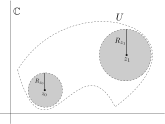
\includegraphics[width=0.5\linewidth]{Figuras/func-analitica-1}
\caption{Nesta figura mostramos como os vários discos de convergência, das expansões em série de potencias de uma função analítica $f$ definida em $U$ poderiam ter raios distintos.}
\label{fig:func-analitica-1}
\end{figure}


Duas observações são importantes neste momento. Primeiro, em geral, 
os coeficientes $a_n$ podem depender da escolha do ponto $z_0$
e talvez o mais apropriado fosse denotar estes coeficientes por $a_n(z_0)$,
para se deixar mais explícito que há esta dependência.
Segundo, se $f:U\to\mathbb{C}$ é uma função analítica, então 
como consequência do Teorema \ref{teo-diff-serie-pot-centro-z0}, 
temos que $f$ possui infinitas derivadas, 
em qualquer ponto de seu domínio e, além do mais, o 
Corolário \ref{cor-serie-taylor-para-serie-pot-centro-z0} afirma que 
\[
a_n \equiv a_n(z_0) = \frac{f^{(n)}(z_0)}{n!}, \qquad \forall n\in\mathbb{N}\cup\{0\}.
\]


Um dos principais resultados desta seção afirma 
que uma série de potências centrada em $w\in\mathbb{C}$, 
com raio de convergência $R_{w}>0$; 
define em seu disco de convergência uma função 
$f:D(w,R_{w})\to\mathbb{C}$ que é analítica. 

Para provar este resultado precisaremos 
enunciar e provar alguns fatos auxiliares sobre troca de ordem de
somas infinitas e a fórmula do Binômio de Newton para váriáveis complexas. 

É importante observar que analiticidade de uma função definida por 
uma série de potências também pode ser obtida 
como consequência da Fórmula Integral de Cauchy. 
Na verdade, no contexto de variáveis complexas, diria que esta
seria a rota mais natural para provar este fato. 
Mas isto requer ferramentas que só serão vistas mais a frente, 
quando estivermos apresentando a teoria de integração complexa. 

Uma vantagem da abordagem desenvolvida nesta seção é que ela se adapta
muito facilmente para outros contextos mais gerais 
em que também podemos definir séries de potências, mas não dispomos
de uma ferramenta como a Fórmula Integral de Cauchy.
Por exemplo, podemos aplicar as ideias desta seção 
para estudar analiticidade de séries de potências definidas
em certos espaços de Banach de dimensão infinita. 

\begin{teorema}\label{teo-fubini-discreto}
Para cada par $n,m\in \mathbb{N}\cup\{0\}$ seja $a_{n,m}$ um número complexo.
Suponha que para cada índice $n\in\mathbb{N}\cup\{0\}$ fixado, que a série 
formada pela sequência $(a_{n,m})_{m\in\mathbb{R}\cup\{0\}}$ converge
absolutamente e que a soma dos 
valores absolutos é dada por
\[
\sum_{m=0}^{\infty} |a_{n,m}| = L_n.
\]
Além do mais, assuma que a série formada por estas somas, isto é, 
$\sum_{n=0}^{\infty} L_n = A$ também é convergente. 

Então as seguintes
séries são convergentes e valem as seguintes igualdades:
\begin{itemize}
\item 
$
\displaystyle \sum_{n=0}^{\infty}\sum_{m=0}^{\infty}|a_{n,m}|
=
\sum_{m=0}^{\infty}\sum_{n=0}^{\infty}|a_{n,m}|;
$

\item 
para cada $m\in\mathbb{N}\cup\{0\}$ fixado,\qquad  $\displaystyle \sum_{n=0}^{\infty} a_{nm} \equiv C_m$;

\item 
$
\displaystyle
\sum_{n=0}^{\infty}\sum_{m=0}^{\infty}a_{n,m} 
=
\sum_{m=0}^{\infty}\sum_{n=0}^{\infty}a_{n,m}.
$
\end{itemize}

\end{teorema}

\bigskip 


O Teorema \ref{teo-fubini-discreto} pode ser visto como uma versão do Teorema
de Fubini sobre integrais iteradas. Para isto basta olharmos 
para $a_{n,m}$ como imagem de uma
função de duas variáveis 
$g:(\mathbb{N}\cup\{0\})\times(\mathbb{N}\cup\{0\})\to\mathbb{R}$.
Deste ponto de vista a conclusão do teorema poderia ser interpretada 
como a afirmação de que a soma dupla pode ser vista como
somas iteradas nas primeira e segunda variáveis, respectivamente, 
e que a ordem das somas podem ser intercambiadas. Ou de maneira
mais intuitiva. Se pensamos na lista de $a_{n,m}$'s como uma espécie 
de matrix com infinitas linhas e infinitas colunas. 
O Teorema \ref{teo-fubini-discreto} 
afirma que podemos primeiro somar cada linha desta matriz e em seguida
somar estas somas e que isto é igual a somar as colunas da matriz e 
depois somar estas somas.

\begin{figure}[h]
\centering
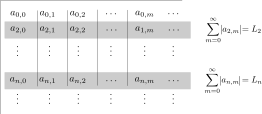
\includegraphics[width=0.75\linewidth]{Figuras/fubini-anm}
\caption{Pensando em toda a lista de $a_{n,m}$'s como uma espécie de matrix com infinitas linhas e infinitas colunas. A hipótese do Teorema \ref{teo-fubini-discreto} é que a soma dos valores absolutos das linhas desta matriz formam um nova sequência $(L_n)_{n\in\mathbb{N}\cup\{0\}}$ cuja a série associada é converge.}
\label{fig:fubini-anm}
\end{figure}


Outra maneira de pensar no Teorema \ref{teo-fubini-discreto} é vendo
que ele se trata de um resultado sobre troca de ordem de limites.
Para deixar isto mais claro vamos reescrever as séries
que aparecem na conclusão deste teorema, como limite de suas somas parciais 
(o que por definição é o que elas realmente são). 


Primeiro observe que
\begin{align}\label{eq-aux1-limite-duplo}
\sum_{n=0}^{\infty}\sum_{m=0}^{\infty}a_{n,m}
=
\lim_{p\to\infty}\sum_{n=0}^{p}\lim_{q\to\infty} \sum_{m=0}^{q}a_{n,m} 
=
\lim_{p\to\infty} \lim_{q\to\infty} \sum_{n=0}^{p} \sum_{m=0}^{q}a_{n,m}, 
\end{align}
onde na última igualdade usamos que para cada $p$ fixado que podemos
permutar a ordem da soma em $n$ com limite em $q$ por causa de uma propriedade
elementar de limite de sequências que afirma que a soma 
dos limites é o limite da soma,
quando cada um dos limites existem. O que justifica a última 
igualdade em \eqref{eq-aux1-limite-duplo}, ou seja,
\[
\sum_{n=0}^{p}\lim_{q\to\infty} \sum_{m=0}^{q}a_{n,m} 
=
\lim_{q\to\infty} \sum_{n=0}^{p}\sum_{m=0}^{q}a_{n,m}. 
\]
\bigskip 


Analogamente, temos 
\begin{align}\label{eq-aux2-limite-duplo}
\sum_{m=0}^{\infty}\sum_{n=0}^{\infty}a_{n,m}
=
\lim_{q\to\infty}\sum_{n=0}^{q}\lim_{p\to\infty} \sum_{m=0}^{p}a_{n,m} 
=
\lim_{p\to\infty} \lim_{q\to\infty} \sum_{n=0}^{q} \sum_{m=0}^{p}a_{n,m}. 
\end{align}

Já que para cada $p,q\in\mathbb{N}$ (finitos) obviamente temos:
\begin{align}
\label{eq-aux3-limite-duplo}
S(p,q) 
\equiv 
\sum_{n=0}^{q} \sum_{m=0}^{p}a_{n,m} 
= 
\sum_{m=0}^{p}\sum_{n=0}^{q} a_{n,m}. 
\end{align}

A grande conclusão do Teorema \ref{teo-fubini-discreto} é que
as expressões do lado direito de \eqref{eq-aux1-limite-duplo}
e \eqref{eq-aux2-limite-duplo} são iguais e consequentemente 
\[
\lim_{p\to\infty} \lim_{q\to\infty} \sum_{n=0}^{p} \sum_{m=0}^{q}a_{n,m}
=
\lim_{q\to\infty}\lim_{p\to\infty} \sum_{n=0}^{p} \sum_{m=0}^{q}a_{n,m}.
\]
Em outras palavras, usando \eqref{eq-aux3-limite-duplo}, podemos simplificar
a expressão acima para
\[
\lim_{p\to\infty} \lim_{q\to\infty} S(p,q)
=
\lim_{q\to\infty}\lim_{p\to\infty} S(p,q).
\]

A igualdade acima aparentemente poderia soar como uma resultado muito natural. 
Porém o seguinte contra-exemplo ilustra como a conclusão do Teorema
\ref{teo-fubini-discreto} é altamente não-trivial.

\begin{exemplo}
Para cada par de números naturais $p,q\in\mathbb{N}$ defina 
\[
S(p,q) =  \frac{p}{p+q}.
\]
Então 
\[
\lim_{p\to\infty} \lim_{q\to\infty} S(p,q)
= 
\lim_{p\to\infty} \lim_{q\to\infty} \frac{p}{p+q}
= 
\lim_{p\to\infty} 0
=0
\]
e por outro lado 
\[
\lim_{q\to\infty}\lim_{p\to\infty} S(p,q)
=
\lim_{q\to\infty} \lim_{p\to\infty} \frac{p}{p+q}
=
\lim_{q\to\infty} 1
=1.
\]
Ou seja, em geral, não podemos inverter a ordem com que tomamos
limites.
\end{exemplo}


O Teorema \ref{teo-fubini-discreto} será uma das principais ferramentas utilizadas 
para mostrar que uma função $f$ dada por uma série
de potências em seu disco de convergência $D(z_0,R)$, com $R>0$,  
é uma função analítica.

A princípio, um leitor mais desatento, poderia inicialmente suspeitar de 
que não há nada a fazer, já que nossa função 
$f:D(z_0,R)\to\mathbb{C}$, por hipótese, é dada
por um série de potências, isto é,
\[
f(z) = \sum_{n=0}^{\infty}a_n(z-z_0)^n. 
\]

Mas alertamos que a questão delicada que se coloca aqui 
é que a definição de analiticidade,
exige que $f$ possa ser expressa como série de potências com raio 
de convergência positivo em torno de qualquer ponto do seu domínio. 
Isto é, dado
$z_1\in D(z_0,R)$ qualquer, diferente de $z_0$, a dificuldade técnica que 
se apresenta é: como garantir
que existem coeficientes $(b_n)_{n\in\mathbb{N}\cup\{0\}}$ 
e $R_{z_1}>0$ tais que $f$ possa ser representada como uma 
série de potências em torno deste novo ponto $z_1$, ou seja,
\[
f(z) = \sum_{n=0}^{\infty} b_n(z-z_1)^n, \qquad \forall z\in D(z_1,R_{z_1}).
\]
Em outras palavras, precisamos entender o que acontece quando mudamos
o ponto onde centramos a expansão em série de potencias de $f$. 
Isto passa por entender como se relacionam os coeficientes de cada 
uma destas expansões bem como os raios dos discos de convergência,
respectivos. 

Antes porém, precisamos de mais um resultado preparatório
que consiste em uma generalização, para números complexos, 
da famosa fórmula do Binômio de Newton

\begin{proposicao}[Binômio de Newton]
\label{prop-binom-newton}
\index{Binômio de Newton}
Para quaisquer $z,w\in\mathbb{C}$ e $n\in\mathbb{N}$ temos 
\begin{align}\label{eq-form-binom-newton}
(w+z)^n = \sum_{k=0}^n \binom{n}{k}z^{k}w^{n-k}, 
\quad \text{onde}\quad \binom{n}{k} = \frac{n!}{(n-k)!k!}.
\end{align}
\end{proposicao}

% \begin{proof}
% Observamos que é possível apresentar uma prova desta proposição 
% usando argumentos idênticos a maioria
% daqueles empregados nas provas em que $z$ e $w$ são 
% números reais. Praticamente os seguindo \textit{ipsis litteris}.  
% Isto porque a maioria destas provas, no caso real, 
% só se utiliza da estrutura de corpo de $\mathbb{R}$
% e das relações de Stifel para os coeficientes binomiais.

% \medskip 

% Por questão de completude, vamos apresentar aqui
% uma prova alternativa da validade desta proposição,
% que é enunciada para números complexos, explorando a fórmula do 
% Binômio de Newton conhecida para números reais. 

% Para isto, primeiro observamos que para todo $x\in\mathbb{R}$, temos
% da fórmula do Binômio de Newton, para números reais, que
% \[
% (1+x)^n = \sum_{k=0}^n \binom{n}{k}x^k.
% \]
% Olhando com cuidado a identidade acima, o leitor pode observar que ela
% revela que $x=-1$ é uma raíz, de 
% multiplicidade $n$, do polinômio $p:\mathbb{R}\to\mathbb{R}$,
% de grau $n$, dado por
% \[
% p(x) = \sum_{k=0}^n \binom{n}{k}x^k.
% \]

% Considere agora a função polinomial $P:\mathbb{C}\to\mathbb{C}$ 
% cujos os coeficientes são os mesmos de $p(x)$, isto é, 
% \[
% P(z) = \sum_{k=0}^n \binom{n}{k}z^k.
% \]
% Já que os coeficientes dos polinômios $p$ e $P$ são os mesmos, temos que 
% $\mathrm{grau}(P)=n$,
% e que $z=-1$ também é uma raíz de $P$ de multiplicidade $n$.
% Pois toda raíz de $p$ é obviamente uma raíz de $P$. Eventualmente, poderíamos imaginar que
% $P$ poderia ter raízes outras complexas com parte imaginária  não-nula.
% Mas isto não pode acontecer por causa do 
% algoritmo de divisão de Euclides para polinômios,
% que garante que $(z+1)^n$ é um fator de $P(z)$. 
% Mas como $\mathrm{grau}(P)=n$ então sua fatoração é exatamente 
% esta $(z+1)^n$. Assim temos
% \[
% \sum_{k=0}^n \binom{n}{k}z^k  = P(z) = (z+1)^n, \qquad \forall z\in\mathbb{C} 
% \]

% Agora podemos usar a identidade acima para 
% verificar a validade de fórmula do Binômio de Newton 
% para quaisquer $z\in\mathbb{C}$ e 
% $w\in\mathbb{C}\setminus\{0,-z\}$. De fato, 
% \begin{align*}
% (w+z)^n 
% = 
% w^n\Big(1+\frac{z}{w}\Big)^n 
% = 
% w^n 
% P\Big(\frac{z}{w}\Big) = 
% w^n
% \sum_{k=0}^n \binom{n}{k}\frac{z^k}{w^k}
% =
% \sum_{k=0}^n \binom{n}{k}z^k\,w^{n-k}.
% \end{align*}

% Para finalizar a prova, basta observar que \eqref{eq-form-binom-newton}
% é obviamente verdadeira nos casos em que $w=0$ ou $w=-z$.
% \end{proof}

\bigskip

Para cada $n\in\mathbb{N}\cup\{0\}$ fixado, considere a função
$\mathds{1}_{[n]}:\mathbb{N}\cup\{0\}\to\{0,1\}$ dada por 
\begin{align}\label{eq-def-1mn}
\mathds{1}_{[n]}(m)
\equiv
\begin{cases}
1,\quad\text{se}\ 0\leqslant m\leqslant n;
\\[0.2cm]
0,\quad\text{caso contrário}.
\end{cases}
\end{align}

Note que a função $\mathds{1}_{[n]}(m)$ assume o valor $1$ se seu argumento  $m\in\{0,1,2,\ldots,n\}$ e assume o valor
zero caso $m>n$. 
Vamos usar estas funções na prova do próximo teorema para expressar somas finitas como 
séries infinitas. Em particular, vamos usar a seguinte identidade
\begin{align}\label{eq-aux1-indicadora-[m]}
\sum_{m=0}^n \mathds{1}_{[n]}(m)\, c_n = \sum_{m=0}^{\infty} \mathds{1}_{[n]}(m)\, c_n,
\end{align}
válida para qualquer $n\in\mathbb{N}\cup\{0\}$ fixado e $(c_n)_{n\in\mathbb{N}\cup\{0\}}$ qualquer sequência de números complexos
(observe que nesta identidade não é preciso nem mesmo 
exigir que a serie dos $c_n$'s seja convergente). 
Na verdade, 
nesta identidade a série que aparece no lado direito 
têm todos os termos de índice maior que $n$
nulos, pela definição de $\mathds{1}_{[n]}(m)$. 

Outra identidade importante na prova do próximo teorema 
e que segue diretamente da definição de $\mathds{1}_{[n]}(m)$ é a seguinte: 
para cada $n\in\mathbb{N}\cup\{0\}$ fixado temos
\begin{align}\label{eq-aux2-indicadora-[m]}
\sum_{m=0}^{\infty} 
\mathds{1}_{[n]}(m)\, c_n 
= 
\sum_{m=n}^{\infty} \mathds{1}_{[n]}(m)\, c_n.
\end{align}


Finalmente estamos prontos para mostrar o resultado mais importante
desta seção.

\bigskip 

\begin{teorema}\label{teo-series-pot-analiticas}
Se $f:D(z_0,R)\to\mathbb{C}$ é uma função definida 
por uma série de potencias, com coeficientes complexos 
$(a_n)_{n\in\mathbb{N}\cup\{0\}}$, centrada
em $z_0\in\mathbb{C}$, com raio de convergência $R>0$. Ou seja,
\[
f(z) = \sum_{n=0}^{\infty} a_n(z-z_0)^n, \qquad \forall z\in D(z_0,R).
\]
Então $f:D(z_0,R)\to\mathbb{C}$ é uma função analítica, isto é, 
para qualquer $z_1\in D(z_0,R)$ fixado, existem 
coeficientes complexos $(b_n)_{n\in\mathbb{N}\cup\{0\}}$ 
e um número positivo $R_{z_1}=R-|z_1-z_0|$
tais que 
\[
f(z) = \sum_{n=0}^{\infty} b_n(z-z_1)^n, \qquad \forall z\in D(z_1,R_{z_1}).
\] 
\end{teorema}

\begin{figure}[h]
\centering
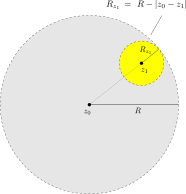
\includegraphics[width=0.55\linewidth]{Figuras/Rz1-func-analitica}
\caption{O raio de convergência da série de potencias centrada em $z_1$ é pelo menos $R_{z_1}=R-|z_0-z_1|$.}
\label{fig:rz1-func-analitica}
\end{figure}


\begin{proof}
Vamos decompor a prova em duas partes. Na primeira parte vamos assumir
que a série de potências está centrada na origem, isto é, $z_0=0$. 
Em seguida, vamos mostrar que o caso geral, $z_0\in\mathbb{C}$ qualquer, 
pode ser reduzido ao caso tratado na primeira parte, 
fazendo uma simples mudança de variáveis.

\bigskip 
\noindent\textbf {Parte 1.}
Como mencionado acima, vamos assumir nesta primeira parte da prova que 
\[
f(z) = \sum_{n=0}^{\infty} a_n z^n, \qquad \forall z\in D(0,R). 
\]
Fixado um ponto arbitrário $z_1\in D(0,R)$ defina $R_{z_1}\equiv R-|z_1|$.


\medskip 

Para cada $m,n\in \mathbb{N}\cup\{0\}$ defina
\[
a_{n,m} = \mathds{1}_{[n]}(m) \cdot a_n \cdot \binom{n}{m} z_1^{n-m}(z-z_1)^{n}, 
\]
onde $\mathds{1}_{[n]}(m)$ é definido como em \eqref{eq-def-1mn}.


Vamos mostrar que os $a_{n,m}$'s satisfazem as hipóteses 
do Teorema \ref{teo-fubini-discreto}, se tomamos $z\in D(z_1,R_{1})$,
onde $R_1=R-|z_1|$. 
Para provar isto, primeiro observamos que 
\[
|a_{n,m}| 
= 
\mathds{1}_{[n]}(m) \cdot |a_n| \cdot \binom{n}{m} |z_1|^{n-m}(|z-z_1|)^{n}. 
\]
E portanto segue da igualdade \eqref{eq-aux1-indicadora-[m]} e da fórmula do Binômio
de Newton (Proposicão \ref{prop-binom-newton}) que para cada  $n\in \mathbb{N}\cup\{0\}$
fixado temos
\begin{align*}
L_n 
\equiv 
\sum_{m=0}^{\infty}|a_{n,m}| 
&=
\sum_{m=0}^{\infty}\mathds{1}_{[n]}(m) \cdot |a_n| \cdot \binom{n}{m} |z_1|^{n-m}(|z-z_1|)^{n} 
\\
&=
\sum_{m=0}^{n} |a_n| \cdot \binom{n}{m} |z_1|^{n-m}(|z-z_1|)^{n} 
\\
&=
|a_n| \sum_{m=0}^{n} \binom{n}{m} |z_1|^{n-m}(|z-z_1|)^{n} 
\\
&=
|a_n| (|z-z_1|+|z_1|)^{n}. 
\end{align*}
Agora note que se tomamos $z\in D(z_1,R_{1})$, então temos $|z-z_1|<R-|z_1|$ e portanto 
$|z-z_1|+|z_1|<R$. Logo temos das propriedades elementares de séries de potencia 
que a série abaixo é convergente
\begin{align*}
\sum_{n=0}^{\infty} L_n = \sum_{n=0}^{\infty} |a_n| (|z-z_1|+|z_1|)^{n}.
\end{align*}
O que mostra que as hipóteses do Teorema \ref{teo-fubini-discreto} são
válidas desde que $z\in D(z_1,R_{1})$. 

\bigskip 
Portanto sob a condição $z\in D(z_1,R_{1})$ poderemos aplicar o Teorema \ref{teo-fubini-discreto} e com isto garantir
a convergência de todas as séries que aparecem abaixo bem como a mudança de 
na ordem das somas feita na nona igualdade abaixo. 
Para facilitar a compreensão pelo leitor, 
observamos também que para a sexta igualdade
que aparece abaixo basta usar \eqref{eq-aux1-indicadora-[m]} e para penúltima
igualdade é só aplicar \eqref{eq-aux2-indicadora-[m]}
\begin{align*}
f(z)
&=
\sum_{n=0}^{\infty} a_nz^n
=
\sum_{n=0}^{\infty} a_n(z-z_1+z_1)^n
\\
&=
\sum_{n=0}^{\infty} a_n \left[ \sum_{m=0}^n \binom{n}{m}z_1^{n-m}(z-z_1)^m  \right]
=
\sum_{n=0}^{\infty}  \left[ \sum_{m=0}^n a_n\binom{n}{m}z_1^{n-m}(z-z_1)^m  \right]
\\
&=
\sum_{n=0}^{\infty}  \left[ \sum_{m=0}^n 
\mathds{1}_{[m]}(n)\cdot a_n\cdot \binom{n}{m}z_1^{n-m}(z-z_1)^m  \right]
\\
&=
\sum_{n=0}^{\infty}  \left[ \sum_{m=0}^{\infty} 
\mathds{1}_{[m]}(n)\cdot a_n\cdot \binom{n}{m}z_1^{n-m}(z-z_1)^m  \right]
\\
&=
\sum_{n=0}^{\infty}  
\sum_{m=0}^{\infty} 
\mathds{1}_{[m]}(n)\cdot a_n\cdot \binom{n}{m}z_1^{n-m}(z-z_1)^m  
\\
&=
\sum_{n=0}^{\infty}  
\sum_{m=0}^{\infty} 
a_{n,m}
=
\sum_{m=0}^{\infty} 
\sum_{n=0}^{\infty}  
a_{n,m}
\\
&=
\sum_{m=0}^{\infty} \sum_{n=0}^{\infty} 
\mathds{1}_{[n]}(m)\cdot a_n\cdot \binom{n}{m}z_1^{n-m}
(z-z_1)^m
\\
&=
\sum_{m=0}^{\infty}  \left[ \sum_{n=0}^{\infty} 
\mathds{1}_{[n]}(m)\cdot a_n\cdot \binom{n}{m}z_1^{n-m}  \right]
(z-z_1)^m
\\
&=
\sum_{m=0}^{\infty}  
\left[ 
\sum_{n=m}^{\infty}  a_n\cdot \binom{n}{m}z_1^{n-m}  \right]
(z-z_1)^m
\\
&=
\sum_{m=0}^{\infty} b_m(z-z_1)^m,
\end{align*}
onde na última igualdade usamos a notação
\begin{align}\label{eq-aux1-teo-series-pot-analiticas}
b_m \equiv \sum_{n=m}^{\infty}  a_n\cdot \binom{n}{m}z_1^{n-m}.
\end{align}

\bigskip 

\noindent\textbf {Parte 2.}
Para provar o teorema quando $z_0$ não é necessariamente zero.
Basta consideramos a mudança de variável $w=z-z_0$.

Fazendo isto temos 
\[
\sum_{n=0}^{\infty}a_n(z-z_0)^n 
=
\sum_{n=0}^{\infty}a_n w^n 
\]
com a série à direta, sendo absolutamente convergente para todo $|w|<R$.

Dado $z_1\in D(z_0,R)$ seja $w_1=z_1-z_0$. É claro que pela escolha
de $z_1$ que temos $|w_1|=|z_0-z_1|<R$.

Note que podemos aplicar o resultado obtido na 
primeira parte da prova, para concluir que 
para todo $w\in D(w_1,R-|w_1|)$ temos:
\[
\sum_{n=0}^{\infty}a_n w^n
=
\sum_{n=0}^{\infty}b_n (w-w_1)^n, \qquad \forall |w-w_1|<R-|w_1|.
\]
Lembrando que $w=z-z_0$ e $w_1=z_1-z_0$, concluímos finalmente da
igualdade acima que 
\[
f(z)
=
\sum_{n=0}^{\infty}a_n (z-z_0)^n
=
\sum_{n=0}^{\infty}b_n \big(\,(z-z_0) -(z_1-z_0)\, \big)^n
=
\sum_{n=0}^{\infty}b_n (z-z_1)^n,
\]
para todo $z\in\mathbb{C}$ satisfazendo $|z-z_1|<R-|w_1|=R-|z_0-z_1|$.
\end{proof}

\bigskip

Há varias observações importante que devem ser feitas sobre o teorema que acabamos
de demonstrar. 


\bigskip 


Primeiro, começamos com nossa função $f:D(z_0,R)\to\mathbb{C}$
dada pela série de potências 
\[
f(z)=\sum_{n=0}^{\infty}a_n(z-z_0)^n.
\]
O mais natural aqui, é que $R$ tenha sido tomado como sendo o raio de convergência 
desta série, que é dado por
\[
R = \frac{1}{\displaystyle\limsup_{n\to\infty} \sqrt[n]{|a_n|}}
\]

O Teorema \ref{teo-series-pot-analiticas} mostra que 
quando mudamos o centro da série de potencias então 
passamos de uma representação de
\[
f(z) = \sum_{n=0}^{\infty}a_n(z-z_0)^n,
\quad \text{válida para todo}\  z\in D(z_0,R),
\] 
para uma nova representação
\begin{align}\label{eq-aux-exe-muda-centro-serie}
f(z) = \sum_{n=0}^{\infty}b_n(z-z_1)^n,
\qquad \text{válida para todo}\ z\in D(z_1,R_1).
\end{align}


Como vimos a série acima converge absolutamente em todo ponto do 
disco $D(z_1,R_1)$, onde $R_1=R-|z_0-z_1|$. Portanto, segue do teorema de existência 
do raio de convergência (\,Teorema \ref{teo-exist-raio-conv} item \textit{(iii)}\,) que
\[
R_{z_1} 
\leqslant 
\frac{1}{\displaystyle\limsup_{n\to\infty} \sqrt[n]{|b_n|}}
\equiv 
\widetilde{R}_{z_1},
\] 
veja Figura \ref{fig:raio-func-analitica-muda-centro}. 

A priori não há nada que proíba a desigualdade acima de ser estrita. 
A ocorrência deste fato é inclusive ligada 
a manifestação de um fenômeno muito importante.
Neste caso, a função $f$ irá admitir uma extensão analítica para além do disco $D(0,R)$!
Para esclarecer este comentário, precisamos 
da definição de extensão analítica de uma função. 

\begin{definicao}[Extensão Analítica]
\label{def-ext-analitica}
\index{Extensão!analítica}
Sejam $U\subset\mathbb{C}$ um conjunto aberto não vazio e
$f:U\to\mathbb{C}$ uma função analítica. Dizemos que $f$ admite
uma extensão analítica à um aberto $V\subset \mathbb{C}$,
contendo $U$ estritamente ($U\subsetneq V$), se existe e uma função analítica $F:V\to\mathbb{C}$ 
tal que $F|_{U}= f$. Isto é, a restrição de $F$ ao conjunto $U$ 
é exatamente a função $f$. 
\end{definicao}


Voltando a discussão acima, se ocorrer $R_{z_1} < \widetilde{R}_{z_1}$
temos que a série de potências em \eqref{eq-aux-exe-muda-centro-serie} 
converge em um ponto $z$ que está
fora do disco $D(z_0,R)$, onde, a rigor, não faria muito sentido falar
de $f(z)$, já que este ponto está fora do domínio da função $f$.
Mas esta observação, nos motiva naturalmente, a definir uma extensão 
analítica de $f$ da seguinte forma. O domínio na nossa extensão será o 
o conjunto $V \equiv D(z_0,R)\cup D(z_1,\widetilde{R}_{z_1})$ e a função
$F:V\to\mathbb{C}$ é dada por 
\[
F(z)
=
\begin{cases}
\displaystyle\sum_{n=0}^{\infty}a_n(z-z_0)^n,&\ \text{se}\ z\in D(z_0,R);
\\[0.9cm]
\displaystyle\sum_{n=0}^{\infty}b_n(z-z_1)^n,&\ \text{se}\ z\in D(z_1,\widetilde{R}_{z_1}).  
\end{cases}
\]

\bigskip 

\begin{figure}[h]
\centering
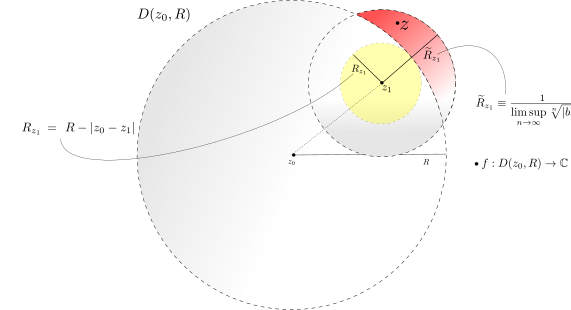
\includegraphics[width=0.95\linewidth]{Figuras/Raio-func-analitica-muda-centro}
\caption{Note que apesar da série de potencias \eqref{eq-aux-exe-muda-centro-serie}, 
centrada em $z_1$ fazer sentido, para qualquer ponto $z$ na região hachurada em vermelho (exterior ao disco $D(z_0,R))$, a rigor, não faz sentido falar de $f(z)$.}
\label{fig:raio-func-analitica-muda-centro}
\end{figure}


Observe que não há ambiguidade na definição acima já que para 
todo $z$ satisfazendo $z\in D(z_0,R)$ e $z\in D(z_1,\widetilde{R}_{z_1})$, isto é, 
\[
z\in D(z_0,R)\cap D(z_1,\widetilde{R}_{z_1})
\] 
temos do Teorema \ref{teo-series-pot-analiticas} que
\[
\sum_{n=0}^{\infty}a_n(z-z_0)^n
=
\sum_{n=0}^{\infty}b_n(z-z_1)^n
\]
e portanto que o valor $F(z)$ está bem definido. 

\medskip 
Claramente temos $F|_{D(z_0,R)} = f$. De fato, se $z\in D(z_0,R)$ segue diretamente das
definições de $F$ e $f$, respectivamente, que 
\[
F(z) = \sum_{n=0}^{\infty}a_n(z-z_0)^n = f(z).
\]

Para verificar que $F$ é analítica precisamos aplicar o 
Teorema \ref{teo-series-pot-analiticas}. 
De fato, para qualquer $z_2\in V= D(z_0,R)\cup D(z_1,\widetilde{R}_{z_1})$ dado,
temos que ou $z_2\in D(z_0,R)$ ou $z_2\in D(z_1,\widetilde{R}_{z_1})$.

\medskip
\noindent
\textbf{Caso 1.} Se $z_2\in D(z_0,R)$ 
então o Teorema \ref{teo-series-pot-analiticas} garante
que existem coeficientes $(c_n)_{n\in\mathbb{N}\cup\{0\}}$ tais que 
\[
F(z) 
= 
\sum_{n=0}^{\infty}a_n(z-z_0)^n 
= 
\sum_{n=0}^{\infty}c_n(z-z_2)^n, \qquad \forall z\in D(z_2,R-|z_0-z_2|).
\]
o que significa que $F$ admite uma representação em séries de potências
centrada em $z_2$ com raio de convergência positivo 
$\widetilde{R}_{z_2} \geqslant R_{z_2}\equiv R-|z_0-z_2|$.

\medskip
\noindent
\textbf{Caso 2.}
Analogamente, se $z_2\in D(z_1,\widetilde{R}_{z_1})$ então temos novamente 
do Teorema \ref{teo-series-pot-analiticas} que existem coeficientes 
$(d_n)_{n\in\mathbb{N}\cup\{0\}}$ tais que 
\[
F(z) 
= 
\sum_{n=0}^{\infty}b_n(z-z_1)^n  
= 
\sum_{n=0}^{\infty}d_n(z-z_2)^n, \qquad \forall z\in D(z_2,\widetilde{R}_{z_1}-|z_1-z_2|).
\]
o que assegura, que também neste caso, $F$ admite uma representação em série
de potências, centrada em $z_2$, com raio de convergência 
$\widetilde{R}_{z_2}\geqslant R_{z_2}\equiv \widetilde{R}_{z_1}-|z_1-z_2|>0$.

\medskip 

Mais a frente, vamos discutir a importante questão 
sobre existência e unicidade de extensões analíticas de uma função.

\medskip


A segunda observação importante sobre o Teorema \ref{teo-series-pot-analiticas}
é que se uma série de potências, centrada em $z_0$, 
tem raio de convergência infinito, ou seja,
se $f:\mathbb{C}\to\mathbb{C}$ é dada por 
\[
f(z) = \sum_{n=0}^{\infty} a_n(z-z_0)^n,\qquad \forall z\in\mathbb{C}
\]
então qualquer que seja $z_1$ em $\mathbb{C}$, existem coeficientes 
$(b_n)_{n\in\mathbb{N}\cup\{0\}}$ tais que 
\[
f(z) = \sum_{n=0}^{\infty} b_n(z-z_1)^n, \qquad \forall z\in\mathbb{C}.
\]
Em outras palavras, se mudamos o centro de uma série de potências 
com raio de convergência infinto, que representa $f$, 
então obtemos uma nova série de potências que representa $f$
e que também tem raio de convergência infinito.


\bigskip

A terceira observação é o seguinte corolário.

\begin{corolario}\label{cor-coeficientes-func-analiticas}
Seja $U\subset\mathbb{C}$ um conjunto aberto e $f:U\to\mathbb{C}$
uma função analítica. Então para cada $z_0\in U$, existe 
$R_{z_0}\in (0,+\infty]$ (positivo estrito) tal que 
\[
f(z) = \sum_{n=0}^{\infty} \frac{f^{(n)}(z_0)}{n!}(z-z_0)^n,
\qquad \forall z\in D(z_0,R_{z_0}).
\]
\end{corolario}

\begin{proof}
Já que $f$ é analítica, temos por definição que para qualquer $z_0\in U$ 
fixado, existem coeficientes $(a_n)_{n\in\mathbb{N}\cup\{0\}}$ e um 
raio de convergência positivo $R_{z_0}$ tais que 
\[
f(z) = \sum_{n=0}^{\infty} a_n(z-z_0)^n,
\qquad \forall z\in D(z_0,R_{z_0}).
\]
Pelo Teorema \ref{teo-diff-serie-pot-centro-z0} e Corolário \ref{cor-serie-taylor-para-serie-pot-centro-z0} a função $f$ 
tem derivadas complexas de todas as ordens e além do mais 
a $n$-ésima derivada de $f$ calculada em $z_0$ satisfaz
\[
a_n = \frac{f^{(n)}(z_0)}{n!}.
\]
\end{proof}



\begin{exemplo}\label{exe-pol-serie-pot}
Se $p:\mathbb{C}\to\mathbb{C}$ é uma função polinomial da forma 
\[
p(z) = a_0+a_1z+a_2z^2+\ldots +a_nz^{n}
\]
então $p$ é uma função analítica.
\end{exemplo}

Escolhemos apresentar e discutir, em detalhes, este exemplo porque
ele ilustra de maneira simples e explícita vários dos conceitos 
e resultados apresentados acima. A ideia apresentada a seguir será fundamental
para estabelecermos vários resultados importantes sobre funções
analíticas. 

\medskip 

Primeiro observe que é possível reconhecer $p$ como 
uma série de potências. 
De fato, considere a sequência $(b_k)_{k\in\mathbb{N}}$
dada por:
\[
b_0=a_0,\quad b_1=a_1,\ \ldots,\quad b_n=a_n,\quad  b_{n+1}=0,\quad b_{n+2}=0,\ \ldots
\]
Então temos para todo $z\in \mathbb{C}$
\[
p(z) = a_0+a_1z+\ldots+a_nz^n = \sum_{k=0}^{\infty} b_kz^k.
\]
Desta forma vemos que $p$ é uma série de potências centrada em zero, com
raio de convergência infinito. Na verdade, esta observação sobre o raio é simplesmente 
uma consequência do lado direito da expressão acima ser uma soma
finita. Este fato óbvio também poderia ser obtido a partir da fórmula 
do raio de convergência, já que, 
\begin{align*}
\limsup_{k\to\infty} \sqrt[k]{|b_k|}
&\equiv 
\lim_{k\to\infty} \left[ \sup \Big\{ \sqrt[k]{|b_k|}, \sqrt[k+1]{|b_{k+1}|}, \sqrt[k+2]{|b_{k+2}|},\ldots  \Big\} \right].
\end{align*}
Pela definição de $b_k$, temos para todo $k>n =\textrm{grau}(p)$ que 
$\sqrt[k]{|b_k|}=0$. Logo a expressão acima, 
é igual a $\lim_{k\to\infty} \sup\{0\} = 0$. Mostrando que
$R^{-1}=0$ e assim $R=+\infty$.  

Aplicando o Teorema \ref{teo-series-pot-analiticas} podemos
concluir que $p$ é uma função analítica. 
Pelas observações feitas acima, podemos mudar o centro da expansão de $p$
para qualquer outro ponto $z_0\in\mathbb{C}$, obtendo novamente outra 
representação em séries de potência para $p$, centrada em $z_0$, com raio 
de convergência também infinito, isto é, existem coeficientes $(c_k)_{k\in\mathbb{N}\cup\{0\}}$ tais que  
\[
p(z) = \sum_{k=0}^{\infty} c_k(z-z_0)^k, \qquad \forall z\in\mathbb{C}.
\]
Do Corolário \ref{cor-coeficientes-func-analiticas} temos que
$c_k= p^{(k)}(z_0)/k!$, para todo $k\geqslant 0$ e
\[
p(z) = \sum_{k=0}^{\infty} \frac{p^{(k)}(z_0)}{k!}(z-z_0)^k, \qquad \forall z\in\mathbb{C}.
\] 
Como as derivadas de $p$ de ordem maiores que $n=\mathrm{grau}(p)$ são nulas, 
temos da igualdade acima que 
\begin{align}\label{eq-polinomio-como-serie-centro-z0}
p(z) = \sum_{k=0}^{n} \frac{p^{(k)}(z_0)}{k!}(z-z_0)^k, \qquad \forall z\in\mathbb{C}.
\end{align}

Para explora só um pouco mais este exemplo, lembramos que identidade 
\eqref{eq-aux1-teo-series-pot-analiticas} fornece uma relação explicita
entre os coeficiente da expansão em série de potencias de uma função 
analítica, quando mudamos o centro da expansão.
Neste caso particular \eqref{eq-aux1-teo-series-pot-analiticas} afirma que
\[
\frac{p^{(k)}(z_0)}{k!}
=
c_k 
= 
\sum_{j=k}^{\infty}  b_j\cdot \binom{j}{k}z_1^{j-k}
=
\sum_{j=k}^{n}  a_j\cdot \binom{j}{k}z_0^{j-k}.
\]

\begin{exemplo}\label{exe-1/z-analitica}
A função $f:\mathbb{C}^{*}\to\mathbb{C}$ dada por 
\[
f(z) = \frac{1}{z}, \qquad \forall z\in\mathbb{C}^{*}
\]
é analítica. 
\end{exemplo}

Para mostrar que $f$ é analítica, 
dado qualquer ponto $z_0\in\mathbb{C}^{*}$ temos que mostrar que
existem coeficientes $(a_n)_{n\in\mathbb{N}\cup\{0\}}$ e 
$R_{z_0}>0$ tais que 
\begin{align}\label{eq-aux3-analiticidade-1/z}
f(z) = \sum_{n=0}^{\infty} a_n(z-z_0)^n, \qquad \forall z\in D(z_0,R_{z_0}).
\end{align}

A ideia vai ser usar séries geométricas, mais precisamente a 
identidade
\begin{align}\label{eq-aux1-analiticidade-1/z}
\frac{1}{1-w} = \sum_{n=0}^{\infty} w^n, \qquad \text{válida para} \ |w|<1.
\end{align}

Dado $z_0\in\mathbb{C}^{*}$, 
observe que podemos escrever, realizando apenas manipulações algébricas simples,
a seguinte igualdade:
\begin{align}\label{eq-aux2-analiticidade-1/z}
\frac{1}{z}
=
\frac{1}{z-z_0+z_0} 
&= 
\frac{1}{\displaystyle z_0\Big( \frac{z-z_0}{z_0}  + 1\Big) } 
\nonumber\\[0.3cm]
&=
\frac{1}{z_0} \frac{1}{\displaystyle\Big( 1+\frac{z-z_0}{z_0}\Big) } 
=
\frac{1}{z_0} \frac{1}{\displaystyle\Big( 1-(-1)\frac{z-z_0}{z_0}\Big) } 
\nonumber\\
&=
\frac{1}{z_0} \frac{1}{\displaystyle\Big( 1-\frac{z-z_0}{-z_0}\Big) } 
\end{align}

Se consideramos apenas os números complexos $z$'s satisfazendo 
\[
\left| \frac{z-z_0}{-z_0} \right|<1, \qquad \text{ou seja},\qquad \ |z-z_0|<|z_0| 
\quad \Longleftrightarrow \quad z\in D(z_0,|z_0|)
\]
Podemos usar identidade \eqref{eq-aux1-analiticidade-1/z} 
na segunda fração que aparece em 
\eqref{eq-aux2-analiticidade-1/z} para concluir que 

\begin{align*}
f(z)
=
\frac{1}{z}
&=
\frac{1}{z_0} \frac{1}{\displaystyle\Big( 1-\frac{z-z_0}{-z_0}\Big) } 
\\[0.3cm]
&=
\frac{1}{z_0}\sum_{n=0}^{\infty} \left( \frac{z-z_0}{-z_0} \right)^n
\\[0.3cm]
&=
\frac{1}{z_0}\sum_{n=0}^{\infty}\frac{1}{(-1)^n \, (z_0)^n} (z-z_0)^n
\\[0.3cm]
&=
\sum_{n=0}^{\infty}\frac{(-1)^n}{(z_0)^{n+1}} (z-z_0)^n,
\qquad \forall z\in D(z_0,|z_0|).
\end{align*}

A identidade acima prova a existência de uma representação 
em série de potências para $f$, em torno de qualquer $z_0\in\mathbb{C}^{*}$, 
com raio de convergência $R_{z_0}=|z_0|>0$
e os coeficientes $a_n$'s dados por 
\[
a_n = \frac{(-1)^n}{(z_0)^{n+1}} ,\qquad \forall n\in\mathbb{N}\cup\{0\},
\]
como exigido em \eqref{eq-aux3-analiticidade-1/z}.


\bigskip

Este exemplo leva a uma observação importantíssima! 
Será que poderíamos ter concluído (apenas com os resultados que provamos até aqui) 
que $f$ é analítica 
simplesmente calculando 
\[
\frac{f^{(n)}(z_0)}{n!} = \frac{(-1)^n}{(z_0)^{n+1}}
\]
e, em seguida, mostrando que este coeficientes nos fornece uma série de
potências convergente com raio de convergência
\[
R 
= 
\frac{1}{\displaystyle\limsup_{n\to\infty} \sqrt[n]{|a_n|}}
=
\frac{1}{\displaystyle\limsup_{n\to\infty} \sqrt[n]{\left|\frac{(-1)^n}{(z_0)^{n+1}}\right|}}
=
\frac{1}{\displaystyle\frac{1}{|z_0|}}
=
|z_0|.
\]

A resposta, a rigor, é não! Até saberíamos que a série de potências
abaixo (que é a série de Taylor de $f$)
\[
\sum_{n=0}^{\infty} \frac{f^{(n)}(z_0)}{n!} (z-z_0)^n
=
\sum_{n=0}^{\infty}\frac{(-1)^n}{(z_0)^{n+1}} (z-z_0)^n,
\quad \text{converge para todo} \ z\in D(z_0,|z_0|).
\]
Mas sem qualquer informação adicional, não teríamos 
como concluir que a série acima, para cada $z$ no disco de convergência,
converge exatamente para $f(z)$. 

\subsection{Princípio da Identidade}

Nesta seção vamos estudar algumas das propriedades fundamentais 
das séries de potências e suas generalizações para funções analíticas
tomando valores em $\mathbb{C}$. 
Um dos principais objetivos é mostrar que se uma função analítica
$f:U\to\mathbb{C}$, definida em um \textbf{domínio} $U$, admite 
uma extensão analítica (no sentido da Definição \ref{def-ext-analitica}) 
à um domínio $V$ contendo $U$, então esta extensão é única.   
Este tipo de resultado mostra claramente a rigidez que a condição 
de analiticidade impõem a uma função. A figura abaixo
ilustra a peculiaridade do resultado mencionado acima, 
já que podemos construir, por exemplo, funções reais deriváveis definidas em 
um intervalo finito $(a,b)$ que 
admitem infinitas extensões deriváveis.



\bigskip 


Para começar vamos considerar as séries de potências mais simples
de todas que àquelas dadas por polinômios.
Seja $p:\mathbb{C}\to\mathbb{C}$ dada por $p(z)=a_0+a_1z+a_2z^2+\ldots+a_nz^n$.
Um polinômio não-nulo de grau $n$. Suponha que $z_0$ é seja uma raiz de $P$ e
considere sua expansão em série de potências em torno de $z=z_0$, obtida no 
Exemplo \ref{exe-pol-serie-pot},
\[
p(z) = \sum_{k=0}^{n} \frac{p^{(k)}(z_0)}{k!}(z-z_0)^k, \qquad \forall z\in\mathbb{C}.
\] 
Já que $p(z_0)=0$, o primeiro termo do somatório acima é nulo e  
portanto podemos reescrever $p$ como segue
\[
p(z)=(z-z_0)\sum_{k=1}^{n} \frac{p^{(k)}(z_0)}{k!}(z-z_0)^{k-1}, \qquad \forall z\in\mathbb{C}.
\]
Procedendo de maneira análoga podemos repetir este processo de fatoração $m$ vezes, 
onde $m$ é determinado pelas seguintes condições:
$p^{(m)}(z_0)\neq 0$, e $p^{(j)}(z_0)=0$ para todo $0\leqslant j\leqslant m-1$. 
Desta forma ficamos com
\[
p(z)=
(z-z_0)^m
\sum_{k=m}^{n} \frac{p^{(k)}(z_0)}{k!}(z-z_0)^{k-m}, \qquad \forall z\in\mathbb{C}.
\]
O valor de $m$ nada mais é do que a multiplicidade de $z_0$ como raíz de $p$.
A razão de apresentá-lo desta maneira é que o método empregado aqui poderá 
ser aplicado também para séries de potências! 

Próximo fato importante que devemos destacar sobre a fatoração obtida acima é que 
o polinômio que aparece como fator de $p(z)$, multiplicando $(z-z_0)^m$, isto é,
\[
q(z) \equiv \sum_{k=m}^{n}\frac{p^{(k)}(z_0)}{k!}(z-z_0)^{k-m} 
\]
é tal que $q(z)$ não se anula em $z=z_0$, pela definição de $m$. 
Já que função $z\longmapsto q(z)$ é contínua dado 
\[ 
\varepsilon = \frac{1}{2}\frac{|p^{(m)}(z_0)|}{m!} 
\]
existe um $\delta>0$ tal que se 
\[
0<|z-z_0|<\delta, 
\quad\text{então}\ \ 
\left| q(z) - \frac{p^{(m)}(z_0)}{m!}\right|
<
\frac{1}{2}\ \frac{|p^{(m)}(z_0)|}{m!}.
\]
Desta forma temos da segunda desigualdade triangular que
\begin{align*}
\left|\frac{p^{(m)}(z_0)}{m!}\right| - |q(z)| 
\leqslant 
\left| q(z) - \frac{p^{(m)}(z_0)}{m!}\right|
<
\frac{1}{2}\ \frac{|p^{(m)}(z_0)|}{m!}
\end{align*}
e portanto 
\[
\frac{1}{2}\ \frac{|p^{(m)}(z_0)|}{m!} <|q(z)|, 
\quad \text{para todo}\ z\ \text{satisfazendo}\ 0<|z-z_0|<\delta.
\]
Mostrando que os zeros de uma função polinomial não-nula 
são isolados. É claro que poderíamos ter chegado a esta mesma conclusão 
por outras vias mais simples. A razão de termos escolhido este argumento é que
ele se generaliza para séries de potências, fornecendo o seguinte
resultado que é de grande importância para a teoria de funções analíticas.


\begin{lema}\label{lema-centro-serie-zero-isolado}
Seja $(a_n)_{n\in\mathbb{N}\cup\{0\}}$ uma sequência de números complexos
não identicamente nula. Suponha que a série de potências 
centrada em $w\in\mathbb{C}$ e gerada por esta sequência, 
tenha raio de convergência $R>0$. 
Seja $f:D(w,R)\to\mathbb{C}$ a função dada por
\[
f(z) = \sum_{n=0}^{\infty}a_n(z-w)^n, \qquad \forall z\in D(w,R)
\]
e denote por $\mathcal{Z}(f)\equiv \{w\in\mathbb{C}: f(w)=0\}$ 
conjunto dos zeros de $f$.  Se o centro da série de potências 
$w\in \mathcal{Z}(f)$ então existe $\delta>0$ tal que 
para todo $z$ satisfazendo $0<|z-w|<\delta$ temos $z\notin \mathcal{Z}(f)$.
Em outras palavras, $w$ é um zero isolado de $f$.
\end{lema}

\begin{figure}[h]
\centering
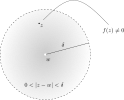
\includegraphics[width=0.45\linewidth]{Figuras/zeros-isolados1}
\caption{O único zero de $f$ dentro do conjunto $\{z\in\mathbb{C}: 0<|z-w|<\delta\}$}
\label{fig:zeros-isolados1}
\end{figure}



\begin{proof}
A prova deste lema é baseada no argumento apresentado no inicio desta seção. 

Suponha que $f(w)=0$. Então temos que $a_0=0$. 
Já que $(a_n)_{n\in\mathbb{N}\cup\{0\}}$ uma sequência de números complexos
não identicamente nula, existe $m\in\mathbb{N}$ (finito),
o primeiro índice, tal que $a_{n}=0$ para todo $0\leqslant n\leqslant m-1$
e $a_{m}\neq 0$. Portanto podemos reescrever $f$ como segue
\begin{align}\label{eq-aux1-principio-ident}
f(z) = (z-w)^{m}\sum_{n=m}^{\infty}a_{n}(z-w)^{m-n}
\equiv (z-w)^{m}g(z).
\end{align}
Note que $g(w)=a_m\neq 0$. Tomando $\varepsilon\equiv |a_m|/2$ segue
da continuidade de $g$ que podemos encontrar um 
$\delta>0$ tal que $B(w,\delta)\subset B(w,R)$ e 
para todo $z$ satisfazendo $0<|z-w|<\delta$ temos $|g(z)-g(w)|<\varepsilon$.
Desta última desigualdade e da segunda desigualdade triangular segue que 
\[
|a_m|-|g(z)|=|g(w)|-|g(z)| \leqslant |g(z)-g(w)|<\varepsilon = \frac{|a_m|}{2}
\quad \Longrightarrow \quad\frac{|a_m|}{2}<|g(z)|,
\]
para todo $z$ satisfazendo $0<|z-w|<\delta$. 
Portanto os dois fatores de \eqref{eq-aux1-principio-ident} não se anulam 
quando para todo $z$ satisfazendo $0<|z-w|<\delta$ e assim $f(z)\neq 0$
sempre que $0<|z-w|<\delta$. O que mostra que $w$ é um zero isolado de $f$.
\end{proof}


\bigskip 

O lema acima prova que se uma série de potências, centrada em $z_0$, 
se anula para $z=z_0$ então $z_0$ é um um zero isolado de $f$. 
O objetivo do próximo lema é preparar o terreno para generalizar
esta afirmação para qualquer zero no disco de convergência da série 
de potências, e não apenas seu centro. 

A estratégia mais natural para se fazer isto seria primeiro aplicar o 
Teorema \ref{teo-series-pot-analiticas} para mudar o centro 
da série de potências para um de seus zeros. Em
seguida, aplicar o lema anterior. 

Há, no entanto, uma dificuldade técnica
de se executar este plano. 
Para exemplificar isto, vamos considerar um caso bem simples, onde 
temos uma série de potências não nula, centrada na origem, 
\[
f(z) = \sum_{n=0}^{\infty} a_nz^n,
\]
que converge em um disco aberto $D(0,R)$, com $R>0$.
Suponha que $z_1$ seja um zero de $f$. 
Aplicando o Teorema \ref{teo-series-pot-analiticas}, podemos mudar o centro 
da expansão acima para $z_1$, isto é, representar $f$ na forma
\[
f(z) = \sum_{n=0}^{\infty} b_n(z-z_1)^n, \qquad \forall z\in D(z_1,R-|z_1|).
\]
Além do mais, podemos invocar a fórmula \eqref{eq-aux1-teo-series-pot-analiticas}.
Esta fórmula fornece, para cada $m\in\mathbb{N}$, uma expressão explicita para $b_m$ em função dos
coeficientes $a_n$'s que é dada por 
\[
b_m \equiv \sum_{n=m}^{\infty}  a_n\cdot \binom{n}{m}z_1^{n-m}.
\]

Se for possível garantir que $b_m\neq 0$, para algum $m\in\mathbb{N}$,
então podemos aplicar o lema acima e garantir que $z_1$ é um 
zero isolado de $f$. O problema é que não é muito claro como 
garantir, pela fórmula acima, 
que a sequência $b_m$ não seja identicamente nula. 
Para contornar este problema vamos provar o seguinte importante resultado.

\begin{lema}\label{lema2-centro-serie-zero-isolado}
Seja $(a_n)_{n\in\mathbb{N}\cup\{0\}}$ uma sequência \textbf{arbitrária} 
de números complexos. Considere que a série de potências, 
centrada em $w\in\mathbb{C}$ e gerada por esta sequência, 
tenha raio de convergência $R>0$. 
Seja $f:D(w,R)\to\mathbb{C}$ a função dada por
\[
f(z) = \sum_{n=0}^{\infty}a_n(z-w)^n, \qquad \forall z\in D(w,R).
\]
Se $f$ se anula em todos os pontos de algum disco aberto 
$D(z_0,r_0)\subset D(w,R)$, com $r_0>0$.
Então $f\equiv 0$ em $D(w,R)$. Em particular, $a_n=0$ para todo $n\geqslant 0$.
\end{lema}

\begin{figure}[h]
\centering
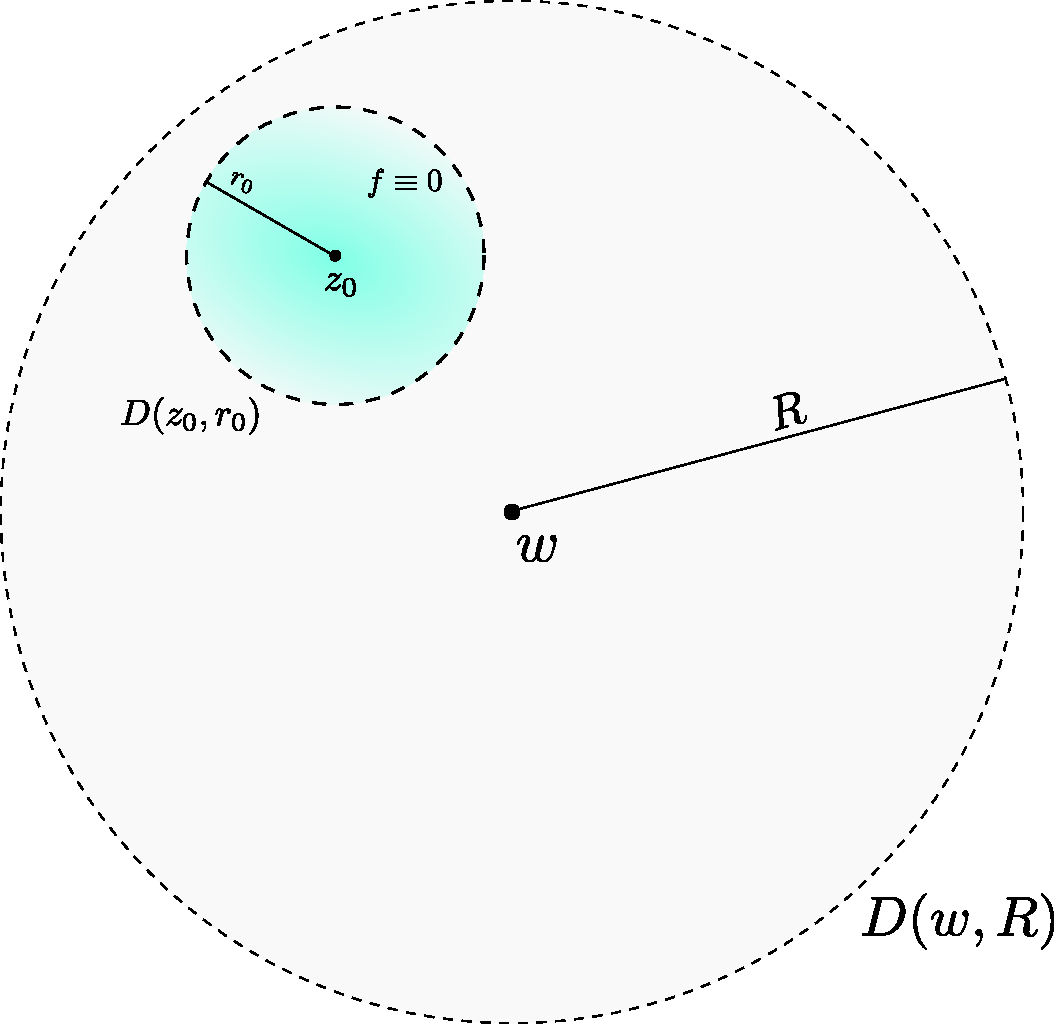
\includegraphics[width=0.6\linewidth]{Figuras/zeros-isolados2}
\caption{A função $f$ se anula em todos os pontos do disco aberto $D(z_0,r_0)$}
\label{fig:zeros-isolados2}
\end{figure}




\begin{proof}
Suponha que exista um disco aberto $D(z_0,r_0)$, com raio $r_0>0$, 
contido em $D(w,R)$ tal que $f(z)=0$ para todo $z\in D(z_0,r_0)$.
Denote por $L_{1}$ o segmento de reta unindo $z_0$ a $w$. 
Seja $z_1$ o único ponto em $L_{1}\cap \partial D(z_0,r_0)$.
Já que $f$ se anula em todos os ponto de $L_1\cap D(z_0,r_0)$ 
e $f$ é contínua em $z_1\in D(0,R)$ segue que $f(z_1)=0$. 
Ou seja, $z_1\in\mathcal{Z}(f)$. 

\begin{figure}[h]
\centering
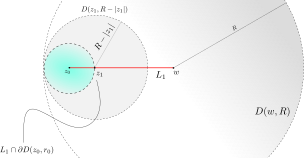
\includegraphics[width=0.6\linewidth]{Figuras/zeros-isolados3}
\caption{Construção da sequência $(z_n)_{n\in\mathbb{N}}$. O primeiro ponto da construção é mostrado acima. Ele é definido como sendo o ponto onde a reta $L_1$ intercepta o disco aberto $D(z_0,r_0)$.}
\label{fig:zeros-isolados3}
\end{figure}




Usando o Teorema \ref{teo-series-pot-analiticas} sabemos que podemos
expandir $f$ em uma série de potências, centrada em $z_1$,
e convergente em todo disco aberto $D(z_1,R-|z_1|)$,
\[
f(z) = \sum_{n=0}^{\infty}b_n(z-z_1)^n.
\]
Já que $z_1\in\mathcal{Z}(f)$ e $f\equiv 0$ em todos os pontos de $L_1$,
segue do Lema \ref{lema-centro-serie-zero-isolado} que $f\equiv 0$
em $D(z_1,R-|z_1|)$. Caso contrário $z_1$ deveria ser um zero isolado de $f$
o que é um absurdo pois $z_1$ é um ponto de acumulação de $L_1$ e 
$f$ se anula em todos os pontos de $L_1$.

 
Se $w\in D(z_1,R-|z_1|)$, não há mais nada a fazer, pois neste
caso existe um $\delta>0$ tal que $D(w,\delta)$
está contido em $D(z_1,R-|z_1|)$ 
e portanto $f\equiv 0$ em $D(w,\delta)$, 
o que implica que todos os coeficientes $a_n$'s da expansão de $f$ em torno
de $w$ são nulos. 


Caso $w\notin D(z_1,R-|z_1|)$, construímos um novo segmento de reta $L_2$
unindo $z_1$ a $w$. Seja $z_2$ o único ponto de interseção entre $L_2$
e $\partial D(z_1,R-|z_1|)$. Argumentando analogamente como acima, verificamos
que $f(z_2)=0$. Usando novamente o Lema \ref{lema-centro-serie-zero-isolado} 
podemos expandir $f$ em uma série de potências, centrada em $z_2$, 
com raio de convergência pelo menos $R-|z_2| = 2(R-|z_1|)>2(R-|z_0|)$.
Já que $z_2\in\mathcal{Z}(f)$ e $f$ se anula em todos os pontos de $L_2$
temos novamente do Lema \ref{lema-centro-serie-zero-isolado} que 
$f\equiv 0$ em $D(z_2,R-|z_2|)$. Como no caso anterior,
se $w\in D(z_2,R-|z_2|)$ não há mais nada a fazer. Caso contrário, 
repetindo os argumentos dados acima, recursivamente, 
até construirmos $z_n$ tal que 
\begin{itemize}
\item
o ponto $z_n$ é o único ponto em $\partial D(z_{n-1},R-|z_{n-1}|)\cap L_n$,
onde $L_n$ é o segmento de reta unindo $z_{n-1}$ a $w$;

\item $f\equiv 0$ em  $D(z_{n},R-|z_{n}|)$;

\item $R-|z_n|= 2^{n-1}(R-|z_1|)$;

\item  $n$ é o menor índice para o qual $w\in D(z_{n},R-|z_{n}|)$.
\end{itemize} 

O que garante a existência de um $n$ finito, satisfazendo a última condição
acima, é o crescimento exponencial obtido no penúltimo item. 

Por construção e pelos teoremas mencionados acima podemos garantir que 
$f$ é identicamente nula no disco $D(z_{n},R-|z_{n}|)$. E portanto
existe algum $\delta>0$ tal que $f$ se nula em todos
os pontos de $D(w,\delta)$. Mas isto implica que todos 
os coeficientes $a_n$'s são nulos e isto encerra a prova deste lema.
\end{proof}



\begin{teorema}[Zeros de Séries de Potência São Isolados]
\label{teo-zeros-series-isolados}
Seja $(a_n)_{n\in\mathbb{N}\cup\{0\}}$ uma sequência de números complexos
\textbf{não identicamente nula}. Suponha que a série de potências 
centrada em $z=z_0$ e gerada por esta sequência tenha raio de convergência $R>0$. 
Seja $f:D(z_0,R)\to\mathbb{C}$ a função dada por
\[
f(z) = \sum_{n=0}^{\infty}a_n(z-z_0)^n, \qquad \forall z\in D(z_0,R).
\]
Então o conjunto de zeros de $f$, notação 
$\mathcal{Z}(f)\equiv \{w\in\mathbb{C}: f(w)=0\}$,
é vazio ou formado apenas por pontos isolados. Isto é, 
para cada $z_1\in \mathcal{Z}(f)$, existe $\delta\equiv\delta_{z_1}>0$ tal que 
se $z$ satifaz $0<|z-z_1|<\delta$ então $z\notin \mathcal{Z}(f)$.
\end{teorema}


\begin{proof}
Caso $f$ não possua zeros, não há nada a fazer. 
Logo só precisamos considerar o caso em que $\mathcal{Z}(f)$ é não-vazio. 
Seja $z_1\in\mathcal{Z}(f)$. Aplicando o Teorema \ref{teo-series-pot-analiticas}
podemos mudar o centro da série de potências de $f$ para o ponto $z=z_1$.
Obtendo assim a seguinte representação de $f$
\begin{align}\label{eq-aux-teo-zero-ser-isol}
f(z)
=
\sum_{n=0}^{\infty} b_n(z-z_1)^{n}, \qquad \forall z\in D(z_1,R_{z_1}).
\end{align}

Pelo Lema \ref{lema2-centro-serie-zero-isolado} podemos garantir 
que para algum $m\in\mathbb{N}$ temos que $b_m\neq 0$. 
De fato, se $b_n=0$ para todo $n\geqslant 0$, então $f$ é identicamente nula em $D(z_1,R_{z_1})$. Mas então segue do
Lema \ref{lema2-centro-serie-zero-isolado} que $f$ também é identicamente nula em 
$D(z_0,R)$. Portanto $a_n=0$, para todo $n\geqslant 0$ o que é uma contradição.

Já que sabemos que algum coeficiente $b_m$ em \eqref{eq-aux-teo-zero-ser-isol} é não-nulo, 
podemos aplicar o Lema \ref{lema-centro-serie-zero-isolado} e assim
garantir que $z_1$ é um zero isolado de $f$, como queríamos demonstrar.
\end{proof}


\bigskip 

\begin{definicao}[Ponto Aderente a um Conjunto]
\label{def-ponto-aderencia}
\index{Ponto!aderente}
Um ponto $z\in\mathbb{C}$ é dito um \textbf{ponto aderente} a um
conjunto $A\subset \mathbb{C}$, se existe uma sequência 
$(z_n)_{n\in\mathbb{N}}$ satisfazendo 
\begin{itemize}
\item $z_n\in A$ para todo $n\in\mathbb{N}$ (os termos da sequência são pontos de $A$);
\item $z_n\neq z_m$, se $n\neq m$ (os termos da sequência são dois-a-dois distintos);
\item $z_n\xrightarrow{\ n\to\infty\ } z$ (a sequência converge para $z$).
\end{itemize}
\end{definicao}



\begin{observacao}
Um ponto $z\in\mathbb{C}$ pode ser um ponto aderente a um conjunto 
$A\subset\mathbb{C}$, mas não ser um ponto de $A$, isto é, podemos
ter um ponto $z$ aderente a $A$ tal que $z\notin A$.

Para um exemplo simples deste caso, considere o seguinte subconjunto de $\mathbb{C}$
\[
A = \Big\{1,\frac{1}{2}, \frac{1}{3}, \frac{1}{4},\ldots\Big\}.
\]
Então é fácil ver que $0$ é aderente a $A$ mas $0\notin A$.
Outro aspecto interessante deste exemplo é que nenhum ponto do
próprio conjunto $A$ é aderente a $A$. 
\end{observacao}

\bigskip 


\begin{teorema}[Principio da Identidade]
\label{teo-principio-identidade}
\index{Principio da Identidade}
Sejam $U,V\subset \mathbb{C}$ domínios não-vazios tais que $U\cap V$ também é um domínio,
não-vazio. Sejam $f:U\to\mathbb{C}$ e $g:V\to\mathbb{C}$ duas funções analíticas. Suponha que
exista um conjunto $I\subset U\cap V$ possuindo um ponto $z_0$ aderente ao conjunto $I$, e 
tal que $f(z)=g(z)$, para todo $z\in I$. 
Então $f(z)=g(z)$ para todo $z\in U\cap V$.
\end{teorema}

\begin{figure}[h]
\centering
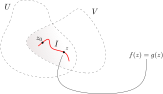
\includegraphics[width=0.65\linewidth]{Figuras/zeros-isolados4}
\caption{O conjunto $I$ onde $f$ e $g$ coincidem é marcado de vermelho. Note que nesta figura $z_0$ é um ponto aderente a $I$. Pois ele pode ser obtido como limite de uma
sequência de pontos que estão em $I$.}
\label{fig:zeros-isolados4}
\end{figure}



\begin{proof}
Vamos dividir a prova deste teorema em duas partes. A primeira parte
mostramos a validade da igualdade $f(z)=g(z)$ em um pequeno disco em torno de $z_0$.
Na segunda parte mostramos como estender a análise local, da primeira parte, 
para todo o domínio $U\cap V$. Este argumento é basicamente um argumento topológico,
mas claro, não apresentado na roupagem de topologia.


\bigskip 
Vale a pena mencionar também que a prova da primeira parte, 
seguirá diretamente dos resultados obtidos
acima, para séries de potências. E seus os argumentos são bem elementares. 
Já a segunda parte, envolve uma argumentação mais sofisticada. 
Numa primeira leitura, a prova da segunda parte pode ser omitida,
sem nenhum prejuízo à compreensão do restante do texto. 

 

\bigskip
\noindent\textbf{Parte 1.}
\\
Por hipótese $z_0\in I$ e além do mais $z_0$ é um ponto aderente a 
$I\subset U\cap V$. 
Já que $f$ e $g$ são analíticas em $U\cap V$ então podemos representar
ambas funções por séries de potências, centradas em $z_0$, com o 
raios de convergência $R_{z_0,f}$ e $R_{z_0,g}$, respectivamente.
Portanto se tomamos $R_{z_0} = \min\{R_{z_0,f},\ R_{z_0,g}\}$ temos que 
\[
f(z) = \sum_{n=0}^{\infty} a_n(z-z_0)^n
\quad \text{e}\ \quad 
g(z) = \sum_{n=0}^{\infty} b_n(z-z_0)^n,
\qquad \forall z\in D(z_0,R_{z_0}).
\]

Segue das propriedades elementares de séries de potência que a diferença das 
séries de potência acima, define uma função $h:D(z_0,R_{z_0})\to\mathbb{C}$
que é dada pela seguinte série de potências:
\[
h(z) \equiv f(z)-g(z) = \sum_{n=0}^{\infty} (a_n-b_n)(z-z_0)^n.
\]
Já que $z_0$ é um ponto aderente a $I$, existe uma 
sequência $(w_n)_{n\in\mathbb{N}}$ de pontos dois-a-dois distintos em $I$ que convergem
para $z_0$. Portanto, para algum $n_0\in\mathbb{N}$ 
temos que $w_n\in D(z_0,R_{z_0})$, para todo $n\geqslant n_0$.
Já que estamos assumindo que $f$ e $g$ coincidem em $I$
então $h(w_n)=0$ para todo $n\geqslant n_0$. 
Desta forma o conjunto de zeros de $h$, ou seja, $\mathcal{Z}(h)$
não é constituído apenas de pontos isolados, pois para todo $n\geqslant n_0$ 
temos que $w_n\in \mathcal{Z}(h)$ e $w_n\xrightarrow{\ n\to\infty\ } z_0\in \mathcal{Z}(h)$.
Logo pelo Teorema \ref{teo-zeros-series-isolados} concluímos que 
os coeficientes da expansão em série de potências de $h$, em torno de $z_0$,
são nulos. E isto mostra que $h\equiv 0$ em $D(z_0,R_{z_0})$.


\medskip
\noindent\textbf{Parte 2.}
\\
Nesta parte, vamos considerar a função $h$ da parte anterior, 
como sendo definida em todo $U\cap V$, isto é, a partir de agora 
$h:U\cap V\to\mathbb{C}$. Sua lei contínua sendo a mesma, ou seja, 
$h(z)=f(z)-g(z)$.

É óbvio que se $D(z_0,R_{z_0})\supset U\cap V$, não há mais nada a fazer. Portanto
vamos assumir que o disco aberto $D(z_0,R_{z_0})$ é um subconjunto estritamente contido
em $U\cap V$. 

%Note que das propriedades elementares de séries de potências 
%segue que $h$ é uma função analítica.
%Diferentemente da primeira parte devemos ficar atentos de que agora agora não é mais 
%possível garantir que exista algum ponto $z_1\in U\cap V$ e um 
%raio positivo $R_{z_1}$ tal que $h$, em todo
%ponto de $U\cap V$, seja representada por uma única série de potências, centrada 
%em $z_1$ com raio de convergência $R_{z_1}$. É claro que $h$ sendo uma função analítica
%ela vai admitir, em cada um dos pontos do seu domínio, uma representação por
%série de potências. Mas tanto os coeficientes quanto o raio de convergência 
%vão depender, em geral, da escolha do ponto em que centramos a série de potências, 
%que irá representar $h$.


\medskip 

Considere o conjunto de zeros da função $h$, isto é,
\[
\mathcal{Z}(h)
\equiv 
\{ z\in U\cap V : h(z)=0 \}.
\]
O objetivo é mostrar que $\mathcal{Z}(h)=U\cap V$. 
Observamos que na Parte 1, foi demonstrado que 
o disco aberto $D(z_0,R_{z_0})$ está completamente contido em $\mathcal{Z}(h)$. 

Seja $z\in U\cap V$ um ponto arbitrário. 
Como estamos supondo que $U\cap V$ é um domínio, podemos
afirmar que existe um caminho, normalizado, injetivo e suave por partes
$\gamma:[0,1]\to\mathbb{C}$ totalmente contido em $U\cap V$
cujos pontos inicial e terminal são $z_0$ e $z$, 
respectivamente. 



Sabemos que $z_0=\gamma(0)\in \mathcal{Z}(h)$ e a ideia, 
desta parte da prova, é mostrar
que $\gamma(t)$, para todo $t\in[0,1]$, está em $\mathcal{Z}(h)$.
A prova deste fato será por contradição. Vamos supor que existe ``um primeiro instante''
antes do tempo $t=1$, em que o caminho $\gamma$ deixa o conjunto de zeros de $h$. E
vamos derivar disto uma contradição.

Para formalizar esta ideia definimos
\[
t^{*} = \sup\big\{ t\in [0,1]:\, \gamma([0,t])\subset \mathcal{Z}(h) \big\}.
\]

O número $t^{*}$ pode ser pensado intuitivamente como 
o ``primeiro instante'' em que a curva $\gamma$ deixa 
o conjunto $\mathcal{Z}(h)$, embora, a rigor,
ele não seja exatamente isto.

\begin{figure}[h]
\centering
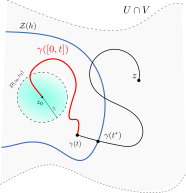
\includegraphics[width=0.55\linewidth]{Figuras/zeros-isolados5}
\caption{Esta figura ilustra a definição de $t^{*}$. A parte em vermelho corresponde a imagem por $\gamma$ do intervalo $[0,t]$ com $t<t^{*}$. Como comentado o ponto $\gamma(t^{*})$ pode ser intuitivamente pensado como o ponto onde o caminho $\gamma$ está prestes a deixar $\mathcal{Z}(h)$.}
\label{fig:zeros-isolados5}
\end{figure}





\medskip 

Na sequência, vamos usar um argumento totalmente análogo ao da Parte 1, 
para mostrar que $\gamma(t^{*})\in \mathcal{Z}(h)$ e, em
seguida, vamos concluir que $t^{*}=1$ e consequentemente que 
$z=\gamma(1)\in \mathcal{Z}(h)$.

\medskip 

Afirmamos que a continuidade de $\gamma$ implica $t^{*}>0$. 
Intuitivamente, o que esta afirmação diz é que toda a ``parte inicial'' 
do caminho $\gamma$ está contida no disco $D(z_0,R_{z_0})$, que por sua vez
está contido em $\mathcal{Z}(h)$. E portanto ``leva'' um tempo positivo para $\gamma(t)$ atingir o bordo do disco $D(z_0,R_{z_0})$. 
De forma precisa, dado $\varepsilon= R_{z_0}$,
segue da continuidade de $\gamma$ em $t=0$ que 
existe $\delta>0$ tal que se $|0-t|=|t|<\delta$ então 
$|z_0-\gamma(t)|=|\gamma(0)-\gamma(t)|<R_{z_0}$. Ou seja, 
$\gamma([0,\delta])\subset D(z_0,R_{z_0})\subset\mathcal{Z}(h)$ e 
consequentemente $0<\delta\leq t^{*}$. Na linguagem informal, usada
acima, o que mostramos é que $\gamma$ não pode deixar o conjunto $\mathcal{Z}(h)$
antes do tempo $t=\delta$. 





\medskip 




Da positividade estrita de $t^{*}$ e da definição de supremo segue 
que existe uma sequência de números positivos
distintos $(t_n)_{n\in\mathbb{N}}$ (estritamente crescente) $0<t_n< t_{n+1}<t^{*}$ tal que $t_n\to t^{*}$, quando $n\to\infty$. 
Invocando novamente a definição de supremo podemos afirmar que 
$\gamma(t_n)\in \mathcal{Z}(h)$, para todo $n\in\mathbb{N}$.
Como $h$ e $\gamma$ são funções contínuas segue que
\[
0
=
\lim_{n\to\infty} h(\gamma(t_n))
= 
h(\gamma(t^{*}))
\]
e consequentemente $\gamma(t^{*})\in\mathcal{Z}(h)$. 

Como $\gamma$ é um caminho totalmente contido em $U\cap V$ temos
que $\gamma(t^{*})\in U\cap V$. Pelo fato da função $h$ ser analítica em 
$U\cap V$, podemos representá-la por uma série de potências, centrada 
em $\gamma(t^{*})$, que converge em 
todo ponto do disco aberto $D( \gamma(t^{*}), R_{\gamma(t^{*})})$, 
com raio $R_{\gamma(t^{*})}$ positivo. 


\begin{figure}[h]
\centering
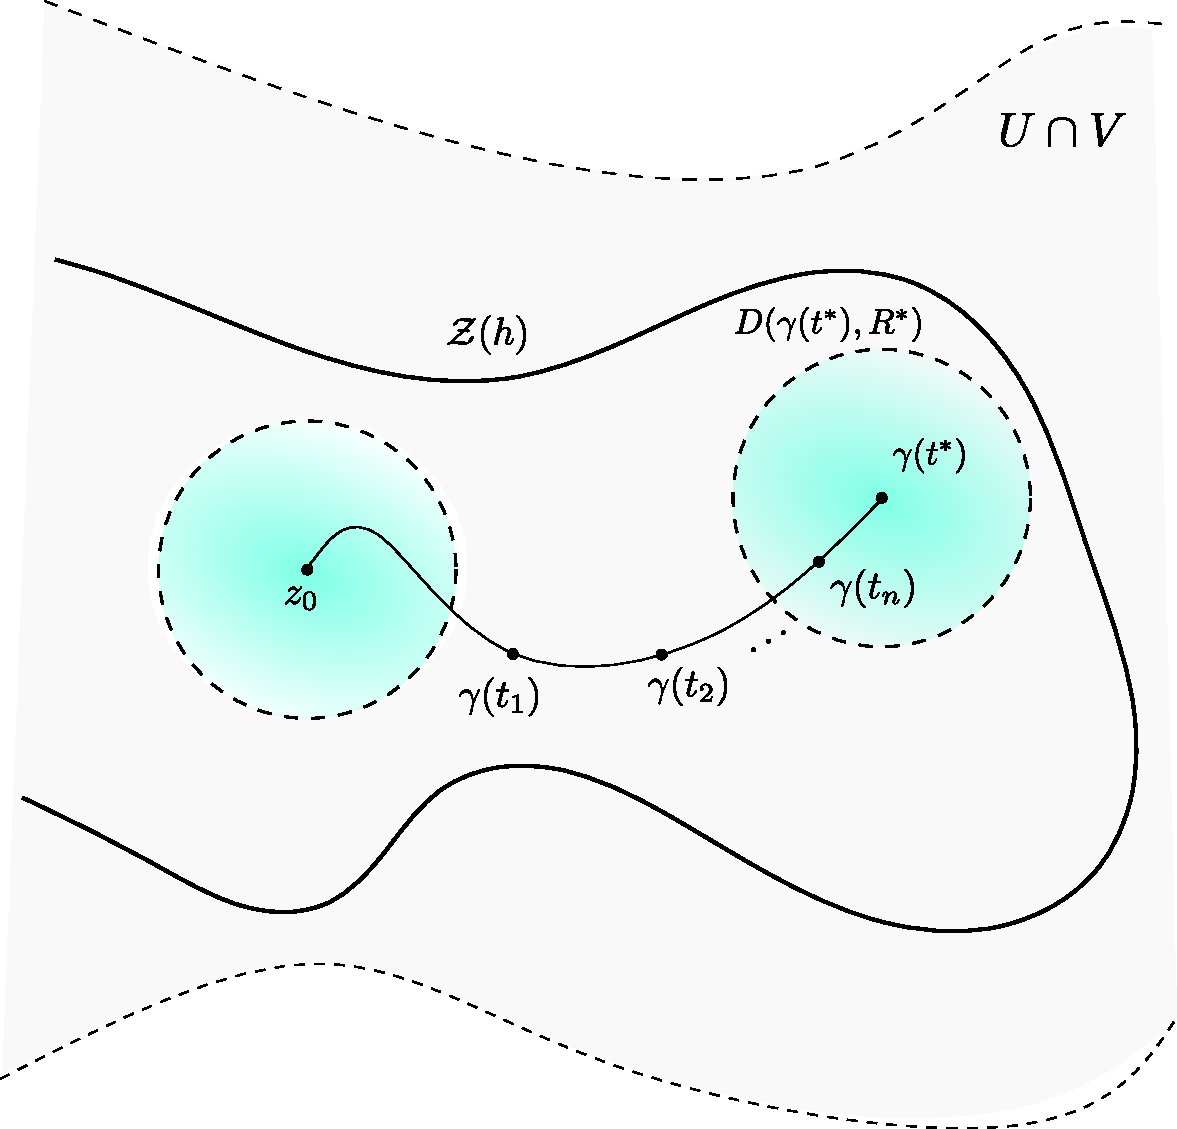
\includegraphics[width=0.6\linewidth]{Figuras/zeros-isolados6}
\caption{O disco $D(\gamma(t^{*}),R^{*})$}
\label{fig:zeros-isolados6}
\end{figure}



Já que $\gamma$ é uma curva injetiva  e $t_n<t_{n+1}$, para todo $n\in\mathbb{N}$,
então os pontos da sequência $(\gamma(t_n))_{n\in\mathbb{N}}$ são todos
distintos. Como $\gamma(t_n)\to \gamma(t^{*})$ temos que $\gamma(t^{*})$
é um ponto aderente ao conjunto $\widetilde{I}\equiv \{\gamma(t^{*}),\gamma(t_1),\gamma(t_2),\ldots\}$.

Argumentando analogamente como na Parte 1, apenas substituindo $I$ por $\widetilde{I}$ 
podemos mostrar que existe algum $R^*>0$ tal que $h\equiv 0$
no disco $D(\gamma(t^*),R^{*})$ e consequentemente que 
$D(\gamma(t^*),R^{*})\subset\mathcal{Z}(h)$.

\medskip 


Depois de todos este preparativos, estamos finalmente prontos para provar que $t^{*}=1$.
De fato, suponha por contradição que $t^{*}<1$. 
Escolhido $\varepsilon = R^{*}$, segue da continuidade de $\gamma$ que 
existe $\delta$ satisfazendo $0<\delta<1-t^{*}$ tal que se $|t-t^{*}|<\delta$ então 
$|\gamma(t)-\gamma(t^{*})|<R^{*}$. Portanto, segue das propriedades
elementares de função ($F(A\cup B)=F(A)\cup F(B)$), da definição de $t^{*}$, 
do argumento de continuidade deste parágrafo e da continência 
$D(\gamma(t^*),R^{*})\subset\mathcal{Z}(h)$
(estabelecida no parágrafo anterior), que 
\begin{align*}
\gamma([0,t^{*}+\delta/2])
=
\gamma([0,t^{*}])\cup \gamma([t^{*},t^{*}+\delta/2])
\subset \mathcal{Z}(h)\cup D(\gamma(t^*),R^{*})
=
\mathcal{Z}(h),
\end{align*}
o que é uma contradição com a definição de $t^{*}$. Como mostramos que $t^{*}$ não pode ser nenhum dos pontos do intervalo $[0,1)$, só resta $t^{*}=1$. Disto segue 
finalmente que $z\in \mathcal{Z}(h)$. Como $z$ foi 
escolhido arbitrariamente em $U\cap V$ segue que $\mathcal{Z}(h)=U\cap V$
e o teorema está finalmente demonstrado.
\end{proof}





\begin{corolario}[Unicidade de Extensões Analíticas]
\label{cor-unicidade-ext-analiticas}
\index{Extensão!analítica}
Sejam $U,V\subset \mathbb{C}$ domínios não vazios, com $U$ estritamente contido em $V$. 
Seja $f:U\to\mathbb{C}$ uma função analítica. Se $F:V\to\mathbb{C}$
e $G:V\to\mathbb{C}$ são funções analíticas que estendem $f$ (extensões
analíticas de $f$), isto é, $F|_{U}=f=G|_{U}$, então $F=G$. 
\end{corolario}


\begin{proof}
A ideia é aplicar o  Teorema \ref{teo-principio-identidade} às funções $F$ e $G$.
Para isto vamos mostrar que todas as hipóteses deste teorema são satisfeitas. 

Primeiro, o teorema citado acima, 
exige que $F$ e $G$ sejam funções analíticas definidas em domínios não-vazios, 
o que é o caso aqui. Ele também exige que $\mathrm{dom}(F)\cap\mathrm{dom}(G)$
seja um domínio não-vazio. Neste caso, esta interseção é precisamente o conjunto $U$,
que por hipótese, é um domínio não-vazio.
Além disto deve, existir um conjunto $I\subset \mathrm{dom}(F)\cap\mathrm{dom}(G)$
possuindo um ponto $z_0$ aderente a $I$, onde $F$ e $G$ coincidem. Neste 
caso o conjunto $I$ pode ser tomado como $I=U=\mathrm{dom}(f)$. De fato,
como $U$ é um domínio não-vazio, dado qualquer ponto $z_0\in U$ 
podemos encontrar um raio $r>0$, tal que que o disco aberto $D(z_0,r)\subset U$.
Logo $z_0$ é um ponto aderente a $U$. Como $F$ e $G$ são extensões de $f$, 
então temos que $F$ e $G$ coincidem em $U$.

Portanto, todas as hipóteses do Teorema 
\ref{teo-principio-identidade} estão garantidas. 
Então ele afirma que $F$ e $G$ coincidem 
em $\mathrm{dom}(F)\cap\mathrm{dom}(G)= V$, e logo $F=G$,
como queríamos demonstrar.
\end{proof}






\begin{exemplo}
Considere a seguinte identidade, bem conhecida, para todo $x,y\in\mathbb{R}$
\begin{align}\label{eq-aux1-form-prod-exp-ext-analitica}
\sum_{n=0}^{\infty} \frac{(x+y)^n }{n!}
=
e^{x+y}
=
e^xe^y
= 
\left( \sum_{n=0}^{\infty} \frac{x^n}{n!} \right)
\left( \sum_{n=0}^{\infty} \frac{y^n}{n!} \right).
\end{align}

Vamos mostrar como as técnicas de extensões analíticas 
(Teorema \ref{teo-principio-identidade})
podem ser usadas para estender a identidade acima para números complexos, isto é,
\[
\sum_{n=0}^{\infty} \frac{(z+w)^n }{n!}
= 
\left( \sum_{n=0}^{\infty} \frac{z^n}{n!} \right)
\left( \sum_{n=0}^{\infty} \frac{w^n}{n!} \right),
\qquad \forall z,w\in\mathbb{C}.
\]

Primeiro, observamos que todas as séries que aparecem acima são convergentes. 
Na verdade, a série de potências dada por
\[
f(z) = \sum_{n=0}^{\infty} \frac{z^n}{n!}
\]
tem raio de convergência
\[
R 
= 
\frac{1}{\displaystyle  \limsup_{n\to\infty} \sqrt[n]{ \frac{1}{n!} } }
=
\limsup_{n\to\infty} \sqrt[n]{ n! }
=+\infty
\]


Fixe $w\in \mathbb{R}$ e considere as funções 
$f_{w}:\mathbb{C}\to\mathbb{C}$ e $g_{w}:\mathbb{C}\to\mathbb{C}$ 
dadas por 
\begin{align*}
f_{w}(z) = \sum_{n=0}^{\infty} \frac{(z+w)^n }{n!}
\quad\text{e}\quad
g_{w}(z) = \left( \sum_{n=0}^{\infty} \frac{z^n}{n!} \right)
\left( \sum_{n=0}^{\infty} \frac{w^n}{n!} \right),
\qquad \forall z\in\mathbb{C}.
\end{align*}

Pelo Teorema \ref{teo-series-pot-analiticas} e pela observação anterior 
é claro que ambas, são funções analíticas
definidas em $\mathbb{C}$. 
Seguindo a notação do Teorema \ref{teo-principio-identidade},
note que se tomamos $I=\mathbb{R}\subset \mathbb{C}$, 
então temos, por exemplo, que $0$ é aderente a $I$ 
e além do mais, para todo $z\in I$, temos que
$f_{w}(z)=g_{w}(z)$. 


\begin{figure}[h]
\centering
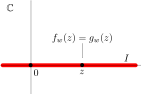
\includegraphics[width=0.4\linewidth]{Figuras/zeros-isolados7}
\caption{Para $z\in\mathbb{R}$ temos que $f_{w}(z)=g_{w}(z)$.}
\label{fig:zeros-isolados7}
\end{figure}



De fato, como $w$ e $z$ são reais e esta igualdade segue imediatamente
de \eqref{eq-aux1-form-prod-exp-ext-analitica}.
Portanto podemos aplicar o  Teorema \ref{teo-principio-identidade}. 
Neste caso ele garante que a igualdade
permanece válida em todo os pontos da interseção dos domínios das funções $f_{w}$ e 
$g_{w}$. Mas como ambas estão definidas em todo plano complexo segue que
$f_{w}(z)=g_{w}(z)$, para todo $z\in \mathbb{C}$. Portanto temos
\begin{align}\label{eq-aux2-form-prod-exp-ext-analitica}
\sum_{n=0}^{\infty} \frac{(z+w)^n }{n!}
=
\left( \sum_{n=0}^{\infty} \frac{z^n}{n!} \right)
\left( \sum_{n=0}^{\infty} \frac{w^n}{n!} \right),
\qquad \forall z\in\mathbb{C} \ \text{e}\ w\in\mathbb{R}.
\end{align}

Para completar a prova da identidade, 
precisamos de mais um passo. Permitir que $w$ seja também
qualquer número complexo. Mas a ideia é a mesma, porém 
agora podemos contar com a vantagem de poder construir as ``funções auxiliares'''
$f_{w}$ e $g_{w}$, fixando números complexos! 

\medskip 

Fixe um número complexo arbitrário $z\in \mathbb{C}$. 
Como o Teorema \ref{teo-series-pot-analiticas}
permite afirmar que qualquer série de potências define em seu raio de convergência
uma função analítica. As seguintes 
funções $F_{z}:\mathbb{C}\to\mathbb{C}$ 
e $G_{z}:\mathbb{C}\to\mathbb{C}$ dadas por 
\[
F_z(w) = \sum_{n=0}^{\infty} \frac{(z+w)^n }{n!}
\quad\text{e}\quad
G_z(w) = 
\left( \sum_{n=0}^{\infty} \frac{z^n}{n!} \right)
\left( \sum_{n=0}^{\infty} \frac{w^n}{n!} \right),
\qquad \forall w\in\mathbb{C}.
\]
são funções analíticas. Repare que $F_z$ deve ser vista como uma série de potências, centrada em $z$, e $G_{z}$ como uma série de potências centrada em zero multiplicada
por uma constante. 


Considerando novamente $I=\mathbb{R}\subset \mathbb{C}$, 
e $0$ como ponto aderente a $I$ temos de 
\eqref{eq-aux2-form-prod-exp-ext-analitica} que 
$
F_{z}(w)=G_{z}(w)
$
para todo $w\in I$. 
Aplicando novamente o Teorema \ref{teo-principio-identidade},
concluímos que $F_{z}(w)=F_{z}(w)$ para todo $w\in\mathbb{C}$. 
Como $z$ é arbitrário podemos afirmar que vale então a seguinte
identidade: 

\begin{align}\label{eq-aux3-form-prod-exp-ext-analitica}
\sum_{n=0}^{\infty} \frac{(z+w)^n }{n!}
=
\left( \sum_{n=0}^{\infty} \frac{z^n}{n!} \right)
\left( \sum_{n=0}^{\infty} \frac{w^n}{n!} \right),
\qquad \forall z,w\in\mathbb{C}.
\end{align}






\medskip 
\noindent
\textbf{Observação}. Apesar deste exercício usar um exemplo simples para
mostrar como se aplicam as técnicas de extensão analíticas, 
só faz sentido ter escolhido este e não outro, 
porque ainda não provamos que a exponencial complexa, definida 
anteriormente por, $\exp(z)\equiv e^{x}(\cos(y)+i\sen(y))$, onde $z=x+iy$,
admite a representação por sua série de Taylor 
\[
\exp(z) = \sum_{n=0}^{\infty} \frac{z^n}{n!}, \qquad \forall z\in\mathbb{C}.
\]
Um roteiro para prova deste fato é apresentado na lista de exercícios. 
Também daremos, mais a frente, outra prova deste fato no texto, após apresentarmos 
a Fórmula Integral de Cauchy.
\end{exemplo}







\begin{exemplo}
Um dos exemplos mais instrutivos sobre extensões analíticas é dado pela 
série geométrica. Como sabemos a série geométrica em $\mathbb{C}$ pode ser 
vista como uma série de potências, centrada em zero e de raio de convergência $R=1$.
Esta série define uma função analítica $f:\mathbb{D}\to\mathbb{C}$ dada por 
\[
f(z) = \sum_{n=0}^{\infty} z^n.
\]
Por outro lado, considere a 
função $g:\mathbb{C}\setminus\{1\}\to\mathbb{C}$ dada por
\[
g(z) = \frac{1}{1-z}.
\]

Também sabemos que
\[
f(z) = \sum_{n=0}^{\infty}z^n  = \frac{1}{1-z} = g(z), \qquad \forall z\in\mathbb{D}.
\]

Em outras palavras, a igualdade acima diz que $f=g|_{\mathbb{D}}$. 
Ou seja, $g$ é uma extensão de $f$. Procedendo analogamente ao Exemplo \ref{exe-1/z-analitica} podemos
mostrar sem dificuldades que a função 
$g:\mathbb{C}\setminus\{1\}\to\mathbb{C}$ é analítica. 
Então o que a igualdade acima nos diz é que $f$ admite uma 
(única - Corolário \ref{cor-unicidade-ext-analiticas}) 
extensão analítica à $\mathbb{C}\setminus\{1\}$. 

Obviamente podemos calcular $g(3)$, substituindo o número complexo $3$ na 
expressão $1/(1-z)$, pois $3$ é um ponto do domínio de $g$. 
Mas apesar de $g$ ser uma extensão de $f$, \textbf{não} faz nenhum sentido
falar em $f(3)$ muito menos escrever 
\[
\sum_{n=0}^{\infty} 3^n = f(3) = g(3) = -\frac{1}{2}.
\]

Este tipo de confusão geralmente é causado pelo frequente abuso de notação
de denotar $f$ e sua extensão pelo mesmo símbolo. Esta não é uma prática
ruim, mas devemos ter sempre em mente que dependendo do ponto em que vamos
calcular a extensão, devemos ser cuidadosos e não 
usar a expressão algébrica da função $f$ inicialmente dada.
Compreender precisamente esta diferença é ainda mais fundamental
para lidar com casos onde a extensão é obtida por algum 
argumento abstrato de existência. Vamos discutir este assunto
mais profundamente e apresentar outros exemplo mais à frente.
\end{exemplo}


\begin{observacao}
No exemplo acima mostramos que $f:\mathbb{D}\to\mathbb{C}$ dada por
\[
f(z) = \sum_{n=0}^{\infty} z^n, \qquad \forall z\in\mathbb{D}
\]
admite uma extensão analíticas à $\mathbb{C}\setminus\{1\}$.
Isto é, 
\[
\sum_{n=0}^{\infty} z^n = \frac{1}{1-z}, \qquad \forall z\in \mathbb{D}.
\]
Por outro lado, vimos no Exemplo \ref{exemplo-divergencia-bordo-disc-conv}
que a série acima diverge para todo $z_0\in \partial\mathbb{D}$. 
Mas observe que para todo 
$z\in \partial\mathbb{D}\setminus\{1\}$ a função $g$ é contínua em todo
$\mathbb{C}\setminus\{1\}$.
Em particular, se $z_0\in\partial\mathbb{D}\setminus\{1\}$ temos
\[
\lim_{z\to z_0}g(z) = \lim_{z\to z_0}\frac{1}{1-z} = \frac{1}{1-z_0}=g(z_0).
\]
Logo o limite acima existe por qualquer caminho. Então podemos tomá-lo
por pontos que estão no interior do disco unitário. 
Dentro do disco unitário sabemos que 
$f=g$, logo temos 
\[
\frac{1}{1-z_0}
=
g(z_0)
=
\lim_{ \substack{z\to z_0 \\ z\in\mathbb{D}\  }  }\ g(z)
=
\lim_{ \substack{z\to z_0 \\ z\in\mathbb{D}\  }  }\ f(z)
=
\lim_{ \substack{z\to z_0 \\ z\in\mathbb{D}\  }  }\ \sum_{n=0}^{\infty} z^n.
\]
Todas as igualdades acima são realmente válidas. 
Mas por que, já que $g$ é um extensão analítica (portanto contínua) de $f$,
agora não temos uma contradição com o fato da série $\sum_{n=0}^{\infty} z^n$
divergir em $z_0$ e ao mesmo tempo $g(z_0)$ estar bem definido? Isto é, 
o que tem de errado em concluir da igualdade acima (absolutamente correta) que
\[
\text{bem definido} \ \longrightarrow  \ g(z_0) = \sum_{n=0}^{\infty}z_0^n
\ \longleftarrow \ \text{diverge}. 
\]

Refraseando a pergunta. Por que a existência de uma extensão analítica para
a série $\sum_{n=0}^{\infty} z^n$, à todo $\mathbb{C}\setminus\{1\}$, em particular, 
à todo disco unitário, exceto $z=1$ não conflita com o fato da 
série ser divergente em todo ponto do bordo do disco unitário?
\end{observacao}
